% ---------------------------------------------------------------------
% Das Dokument kompiliert mit pdflatex und ist auf Basis 
% von Koma-Script entstanden. 
%
% Autor des Templates (für Anmerkungen): 
% Michael von Riegen, riegen@informatik.uni-hamburg.de
%
% Einzelne Code-Teile für das Titelblatt sind aus dem Template 
% von Benjamin Kirchheim entnommen.
%
% 25.05.09, Frank Langanke: Vorlage auf aktuelle KOMA-Version aktualisiert
% 26.05.09, Michael von Riegen: Anmerkung --> aktuelles Koma-Script ist nötig!
% 17.10.2016 neues Uni logo
% ---------------------------------------------------------------------
\documentclass[11pt,DIV=15,BCOR=20mm,bibliography=totoc]{scrbook}

% Import von Paketen und Optionen die das gesamte Dokument betreffen
% sind in myPreamble.sty ausgelagert.
\usepackage{myPreamble}
   
% Arbeitet man nur an einem Kapitel, wird durch folgenden Befehl nur dieses eingebunden.
% Spart manuelles auskommentieren von vielen include-Befehlen;
% hat keine Auswirkung auf input-Befehle
% \includeonly{kapitel1}
   
\begin{document}


\begin{titlepage}

	% Fehler "destination with the same identifier" unterdrücken...
  \setcounter{page}{-1}

	% Titelseite
	\begin{figure}[h]
		\begin{minipage}[b]{62mm}
			
\includegraphics[width=62mm]{images/unilogo}
		\end{minipage}
		\hspace{4cm}
		%\begin{minipage}[b]{59mm}
		%	\includegraphics[width=59mm]{images/minlogo}
		%\end{minipage}
	\end{figure}

	\vfill
	
	\begin{center}
		% Diplomarbeit 
		\noindent { \huge
			Master's Thesis \\
		}
		\vspace{14mm}
		% Titel
		\noindent \textbf{\huge
		Performance-optimized A/B-Testing for E-Commerce-Websites
		}
		\vspace{60mm}	
	\end{center}
	
	\vfill
	
	\noindent \textbf{Aram Yesildeniz} \\
	\noindent \rule{\textwidth}{0.4mm} 
	\noindent{\textrm{aram.yesildeniz@studium.uni-hamburg.de}} \\
	\noindent{\textrm{M. Sc. Informatics}} \\
	\noindent{\textrm{Matr.-No. 6890370}} \\
	\begin{tabbing}
	\hspace{8em} \=  \kill
	1st supervisor: \> Dr. Wolfram Wingerath \\
	2nd supervisor: \> Benjamin Wollmer \\
	~ \\
	Hamburg, 1st of September 2021
	\end{tabbing}
	
	
	% Rückseite der Titelseite mit Zitat
	\newpage 
	\thispagestyle{empty}
	\setcounter{page}{0}

	% wenn man Lust auf ein Zitat hat...
	% ... ansonsten auskommentieren
	~\\ \vfill \noindent 
	A distributed system is one where the failure of some \\
	computer I've never heard of can keep me from getting my work done. \\
	\textit{-- Leslie Lamport}
\end{titlepage}





% VERZEICHNISSE (Inhaltsverzeichnis, Abkürzungen)
% Vorspann einleiten --> Seitennummerierung römisch
\frontmatter

% Inhaltsverzeichnis
\tableofcontents
\cleardoublepage


% Hauptteil einleiten --> Seitennummerierung wieder arabisch
\mainmatter



\chapter{Introduction}

\begin{itemize}
	\item Explain structure and main goal of this thesis
	\item Introduction Chapter: Describe shortly all sections from this chapter and what the reader can expect
	\item Give short outlook to following chapter
\end{itemize}


% -----------------------------------
% -----------------------------------


\section{E-Commerce}


% [Internet]
\subsection{The Internet}

In the last 50 years, a new technology emerged, spread over the entire world and influenced many aspect of most peoples life.
Within the turmoil of the cold war, the United State's Advanced Research Projects Agency (ARPA) established in 1957 a communication network to bring together universities and their researches all around the country in order to be able compete against the USSR.
% cite 2011 COhen
What started as a tool for scientific collaboration evolved a half century later into the internet, a global network and phenomenon, to which every user with a dedicated device has access and can contribute to.
The internet is an integral part, if not the backbone of today's everyday life.
Users of the internet use it for everything, that is sending emails, watching television, chatting with friends, 
order lunch, checking the weather for the next day or renting motorized scooters.

% [Numbers]

In 2021, the internet has 4.66 billion users, which is around 60\% of the world population.\footnote{Following statistics are taken from \url{https://datareportal.com/reports/digital-2021-germany} [14.05.2021]}
Compared to 2020, the number of internet users increased by 7.3\%.
In Europe, more than 90\% of the population are also internet users.
For a developed country like Germany, the numbers are even more impressing:
94\% of the German population are using the internet with an average daily time of over 5h.

Those numbers demonstrate impressive that the internet is an integral part of our daily life.
Along the rise of internet users, transactions and processes falling under the term of e-commerce rise.
Before discussing the term "e-commerce" and take a grasp at its history and types, some statistics are presented to demonstrate the importance of e-commerce.


% [E-Commerce]
\subsection{E-Commerce}

\subsubsection{Introduction}

From the global data report, we can see that over 90\% of the world population visited an online retail site.
Over 76\% of the world population purchased a product online.
For most categories growth is over 15\%.
Again, for a western country like Germany, the numbers are higher:
92.5\% of the german population visited an online retail site and over 80\% purchased a product online.
And the usage is growing: growth of amount spent in category food and personal care is 28.6\%, and 17.6\% for fashion and beauty.

Revenue in e-commerce is constantly growing over the last 20 years, topping to 57.8 billion in 2019.\footnote{\url{https://einzelhandel.de/presse/zahlenfaktengrafiken/861-online-handel/1889-e-commerce-umsaetze} [14.05.2021]}

% [Corona: Even more growth]

The COVID-19 pandemic with its implications had and still has an not negligible impact on the growth of e-commerce.
Several measures were taken to stop the spread of the virus and the number of deaths, one of which was to minimize physical interaction between people.
This leads consequently to a shift of human interactions to the internet.
Along this, e-commerce benefits.
Bhatti et al concludes that "e-commerce enhanced by COVID-19". %cite 2020 bhatti

% [E-Commerce History]
\subsubsection{Short History}

E-Commerce, or electronic commerce, is according to the \textit{Encyclopædia Britannica} about "maintaining relationships and conducting business transactions that include selling information, services, and goods by means of computer telecommunications networks."\footnote{\url{https://www.britannica.com/technology/e-commerce} [19.05.2021]}
In short, e-commerce is about buying and selling products and services via the internet.

% cite hermogeno and check for Tian when paper available:
The success of e-commerce is tightly coupled to the vast advances of internet technology in the past years, like for example the development of the Electronic Data Interchange (EDI) starting from the 1960s, which standardised the communication between two machines.

Personal computers in 1980s and one of the first examples of online shopping is from CompuServe who introduced Electronic Mall in 1984.

Another milestone is Word Wide Web, introduced in 1990 by Tim Berners-Lee, made internet accessible to everyone.
First browser by Tim.

Social media since 2000 again offeres new possibilities for businesses and consumers alike to participate in e-commerce, e.g. for marketing, selling channels

New devices such as smart phones and tablets again decreases the hurdle to participate in e-commerce.
While in the time dimension e-commerce was already available all the time, with the new mobility its also available everywhere.
More flexible.

With the ongoing progress in technology, also e-commerce can expect a shining future with trends such as AI recommendation systems, outstanding UX thanks to Virtual Reality, simple payment methods with crypto etc.\footnote{\url{https://www.spiralytics.com/blog/past-present-future-ecommerce/} [19.05.2021]}


% [Types]
\subsubsection{Types}

Multiple types in e-commerce are existing. They emerge from the possible combinations between the actors \textit{business}, \textit{consumer} and \textit{government}. %cite dos santos

\begin{itemize}
\item B2B: Business to Business
\item B2C: Business to Consumer
\item C2C: Consumer to Consumer
\item G2C: Government to Consumer
\item B2G: Business to Government
\item G2G: Government to Government
\end{itemize}

% [B2C]
\paragraph{B2C}
Business to Consumer in e-commerce describes basically online shopping, by means of a business offering its services and products to the consumer over the World Wide Web.
The consumer can browse within an online shop through the presented products and services and order them directly via the website.
A variety of payment and delivery options conclude the B2C type.
% cite Heinemann p. 75

For a aspiring business, multiple ready to use software solutions to install an online shop are existing, for example. Shopify, ePages, Magento or WooCommerce. % cite Handbuch Online-Shop

% [Amazon]
A famous example of a B2C company is Amazon.
On the 16th of July in 1995, Amazon launched as a website and entered the stock market on the 15th of May 1997.%cite Der Allesverkäufer p. 47
Amazon is successful, the stock started with a price of X, which is at the time of this writing at Y.\footnote{\url{https://finance.yahoo.com/quote/AMZN?p=AMZN} [19.05.2021]}
Today Amazon employs over 1 million employees\footnote{\url{https://www.statista.com/statistics/234488/number-of-amazon-employees/} [19.05.2021]} and serves the wishes of 200 million paying prime members.\footnote{\url{https://www.statista.com/statistics/829113/number-of-paying-amazon-prime-members/} [20.05.2021]}


% [Pro and Con]
By taking a quick look at the pros and cons of maintaining an online shop, we can see that some of the advantages are that there is no need of a real house to present and sell the products, the virtual shop is available to the consumer at any time and has to closing hours; there is a high potential for the online shop as it is part of growing market; online business is scalable; due to tracking algorithms precise targeting as well as data analysis is possible; to start with an online business, not that much float is needed and there are in general lower costs; it is possible to provide a personalized customer experience; 

Some disadvantages are that the speed of market is rapid, competitors arise everyday everywhere, technology evolves quickly while consumers expectations go high.
% cite 2019 hermogeno and % cite erfolgreicher online handel for dummies


% [Performance of online shop is important]
Another downside is that there is no direct or physical concat with the consumer.
As described above, online shopping takes place in the World Wide Web domain.
Consequently, in person interaction between a buyer and a seller is not possible and the shopping event takes place on a website.
Deriving from this fact, the overall virtual user experience needs to be outstanding in order to stay ahead of competition.
The performance of the online shop is one part of the user experience.

In the next section, I will describe the findings between the correlation between user satisfaction and the performance of the retailers web presence.



% ------------------------------------------


\subsection{User Satisfaction and Performance}

% [User Satisfaction]
The aim of this thesis is not to deep dive into terms and concepts or the non-trivial problem of defining user satisfaction, usability or the like.
Therefore the term user satisfaction is in this context loosely defined as how happy the user is with the website he or she interacts with.\footnote{For a discussion cf. "User satisfaction measurement" in } %cite 2010 Islam

% [Performance]
For this context, performance can be understood as the the speed of an online shop, e.g. how long it takes the page to load, how quickly the user can interact with the page, and how the user perceives the performance of the website.
Later we will see that measuring performance is not that trivial and a lot of ideas and metrics are existing to measure it.

% [SpeedHub]
% QUESTION: should i cite only the keynote or the literature used in the keynote directly ?
\subsubsection{SpeedHub}
A plethora of information and studies about the phenomenon of user satisfaction and web site performance is collected at \textit{SpeedHub.org}, a portal by \textit{Baqend} in cooperation with \textit{Google} which provides "the largest systematic study of Mobile Site Speed and the Impact on E-Commerce."\footnote{\url{https://www.speedhub.org/} [21.05.2021]}
On the hub, not only studies and reports are available, but also collections of videos and blog posts.

% [code.talks 2019]
In his presentation at code talks 2019, Felix Gessert summarizes the findings and provides insights to the most relevant aspects and questions of the study: %cite 2019 Gessert

% [User Profile and Psychology]
The first observation when tackling the question regarding a correlation between the performance of a system and the user satisfaction, is that the users have to be distinguished which leads to the concept of a \textit{User Profile}: Regarding gender, young woman are the most demanding consumers and buy less on slow pages.
Generally, people between 18 and 24 have higher expectations regarding site speed than their older counterparts.
There are also differences between nations and regions, for example people from Japan have the highest expectations, which for a certainty coheres with the technological progress in this country.
Not only the expectations themselves differ geographically, but also how speed influences the users, for example "speed influences New Yorkers more than Californians."

What all users have in common is their human psychology. With respect to performance, researchers generally suggest to keep waiting times under 1000 ms in order to keep the users attention.

% [Devices]
After considering the user itself, the next step is to investigate the influence of the device in use: Studies show that mobile users are more likely to buy products and services than their colleagues using a desktop computer, where iOS users have generally more expectations regarding site speed.
 
% [Context]
Last but not least is the context and the users condition important, where naturally relaxed and calm users perceive sites faster than stressed users or people that are in a hurry.
Also when on the move, users experience sites slower.

% [Studies]
There are many real world examples and studies existing which prove and demonstrate the importance of site speed with respect to user satisfaction and eventually revenue:
\textit{Amazon} fount out that a decrease of 100 ms in page loading leads to -1\% conversion rates.
If the site loads 100 ms faster, \textit{Walmart} observed that the revenue increases by 1\%.
For \textit{Zalando}, increasing site speed by 100 ms leads to an uplift of 0.7\% revenue per session.

% [SEO]
Search Engine Optimization is heavily impacted by load speed:
For \textit{Google}, 500 ms slower sites lead to a decrease of 20\% in traffic.
\textit{GQs} traffic increased by 80\% after the page load went down from 7 s to 2 s.
And for \textit{Pinterest}, 40\% faster loads led to 15\% more SEO traffic.

% [Engagement & Satisfaction]
Also the user engagement and satisfaction rely heavily on load times:  \textit{Forrester} noted an increase of 60\% for the session length while brining down the load time 80\%.
\textit{Akamai} monitored that the bounce rate climbed up incredible 103\% when the load time increased by 2 s.
And for the \textit{AberdeedGroup}, the customer satisfaction dropped by 16\% at one more second delay in response times.

To summarize, many studies and real world examples prove and demonstrate that faster web sites and online shops cause a better user experience and typically lead to happier customers. 
Concluding in commercial terms, one can say with certainty that page speed equals money.
\\

A scientific method is needed in order to test the impact of performance on the users.
One of them is A/B Testing, which is the content of the next section.
After a discussion of A/B Testing, I will move on to the examination of Web Analytics, a term which subsumes methods, tools and instruments for businesses to better understand their business and customers.


\subsubsection{A/B Testing}

% How to quantify, measure impact of performance?
% Try to be scientifically solid

% 2012 Kessler 17.2  AB Tests



% 2016 Kohavi

% 2017 Kohavi
% 2018 Morys
% 2018 Fabijan
% 2020 Heinemann 4.1.4





% ------------------------------------------------------------------------------------
% ------------------------------------------------------------------------------------



\section{Web Analytics}

\begin{itemize}
\item Historical background and contextualisation, usage, definition
\item Web Analytics Process
\item Mechanisms, Measurement methods / Collecting data: Log file analysis, client site page tagging, alternatives
\item KPIs ?
\end{itemize}


\subsection{Introduction}

% Definitions:
% -----------


% 2011 Nakatani:
% Web analytics is used to understand online customers and their behaviors, design actions influential to them, and ultimately foster behaviors beneficial to the business and achieve the organization’s goal.


% 2014 Singal: "Web Analytics is the objective tracking, collection, measurement, reporting and analysis of quantitative internet data to optimize websites and web marketing initiatives."

% 2015 Bekavac:

% "According to the official definition of [13], web analytics refers to a combination of (a) measuring, (b) acquisition, (c) analyzing and (d) reporting of data collected from the Internet with the aim of understanding and optimizing web experience."

% "the analysis of qualitative and quantitative data on the website in order to continuously improve the online experience of visitors, which leads to more efficient and effective realization of the company’s planned goals"




\subsection{Short History}


% 2009 Croll p. 69
% 2009 Jansen ch. 3

% 2014 Singal
% - Genesis of Web Analytics (nice graphic) with WAA, DAA
% - History of tools

% 2015 Zheng
% 2015 Bekavac
% 2019 Hussaina
% 2019 Kumar


\subsection{Web Analytics Process}
% Process:
% --------


% 2009 Jansen ch. 6.2
% 2009 Waisberg
% 2012 Kumar

% 2015 Bekavac:
% - Copies from Waisberg and Kaushik


% 2019 Hussaina
% 2019 Kumar


% Log vs Page tagging:
% --------------------


% 2009 Waisberg

% Hassler ch. 2

% Wolle Draft

% 2011 Marek


% 2011 Nakatani: Pros and cons


% 2014 Singal provides table with pros and cons

% 2015 Bekavac

% 2019 Kumar



% KPIs:
% -----

% 2014 Singal describes KPIs for different businesses

% 2015 Bekavac:
% - KPI definition as part of web analytics process
% - Table with KPIs related to business model


\subsection{Web Performance}

\begin{itemize}
\item What is web performance? Why it matters
\item Overview of factors that impact performance, bottlenecks
\item Overview of measurement methods, techniques and metrics
\end{itemize}



% Bottlenecks of performance, big picture:
% 2013 Grigorik: Latency as bottleneck and not bandwith
% 2016 Witt




\subsection{Tools}

% TODO: move this to related work ?

\begin{itemize}
\item Some short overview about existing tools
\item Conclude that I use WPT for synthetic performance testing and GA for RUM
\end{itemize}

% 2011 Marek: Choose a program



% 2011 Nakatani:
% "Web analytics tools collect click-stream data, track users navigation paths, process and present the data as meaningful information.
% - Categorizations:
% 1: By 4 different data collection methods
% 2: SaaS vs in-house
% 3: mobile vs non-mobile
% 4: Time lag



% 2015 Bekavac
% - 5 categories of tools
% - Process of selecting tool
% - Table with features of tools


% 2016 Bartuskova: 1.2 Services for Website Speed Testing
% 2016 Kaur: Tools for Measuring the Performance of Websites
% 2019 Hussaina
% 2019 Kumar

% 2020 Quintel: Matomo
% Lighthouse Performance Scoring

% 2020 Heinemann 4.1.4




% -----------------------------------
% -----------------------------------



\section{Research Question}

\begin{itemize}
\item Difficulty of defining scope
\item Measuring performance of a web site impacts its performance or other effects take place / Observer effect
\item Why the research question is relevant
\end{itemize}


% Tools: Kessler 2016 p. 576

% Measuring Real User Performance in the Browser: Avoiding the Observer Effect


























\chapter{Introduction to E-Commerce and Web Analytics}

[tbd]




% ---------------------------------------------------------------------------------------------------------



\section{E-Commerce}
\label{chapter:e-commerce}

This chapter gives an introduction to e-commerce.
Before going into the details, the emergence of e-commerce is described, starting with the Internet in section \ref{chapter:internet}.
In the following, I will briefly discuss the history of e-commerce and its types in section \ref{chapter:ecommerce_subchapter}.
The relationship between user satisfaction and the website performance is covered in section \ref{chapter:user_satisfaction}, which then leads to the chapter \ref{chapter:web_analytics} which is about web analytics.



\subsection{The Internet: Overview}
\label{chapter:internet}

In the last 50 years, a new technology emerged, spread over the entire world and influenced many aspects of most peoples life.
Within the turmoil of the cold war, the United State's \textit{Advanced Research Projects Agency} (ARPA) established in 1957 a communication network to bring together universities and their researches all around the country in order to be able compete against the USSR \cite{2011Cohen}.
What started as a tool for scientific collaboration evolved half a century later into the \textit{Internet}, a global network and phenomenon, to which every user with a dedicated device has access and can contribute to.
The internet is an integral part, if not the backbone of today's everyday life.
Users of the internet use it for almost everything, from sending emails, watching television, chatting with friends,  order lunch, checking the weather for the next day or renting motorized scooters.

% [Numbers]
In 2021, the internet has 4.66 billion users, which is around 60\% of the world population.\footnote{Following statistics are taken from \url{https://datareportal.com/reports/digital-2021-germany} [14.05.2021]}
Compared to 2020, the number of internet users increased by 7.3\%.
In Europe, more than 90\% of the population are internet users.
For a developed country like Germany, the numbers are even more impressing:
94\% of the German population are using the internet with an average daily time of over five hours.

Those numbers demonstrate impressive that the internet is an integral part of our daily life.
Along the rise of the internet, transactions and processes falling under the term of e-commerce are climbing as well.
Before discussing the term "e-commerce" and take a grasp at its history and types, some statistics are presented to demonstrate the importance of e-commerce.


\subsection{E-Commerce}
\label{chapter:ecommerce_subchapter}


\subsubsection{Introduction}

From the global data report\footnote{\url{https://datareportal.com/reports/digital-2021-germany} [14.05.2021]}, one can read out that over 90\% of the world population visited an online retail site and over 76\% of the world population purchased a product online.
% For most of the categories growth is over 15\%.  %TODO which categories ?
As usual, for or a western country like Germany, the figures are higher:
92.5\% of the German population visited an online retail site and over 80\% purchased a product online.
And the usage is expanding: the growth of the amount spent within the category food and personal care is 28.6\%, and 17.6\% for the category fashion and beauty.

E-commerce sales have grown steadily over the past 20 years, topping to 57.8 billion in 2019.\footnote{\url{https://einzelhandel.de/presse/zahlenfaktengrafiken/861-online-handel/1889-e-commerce-umsaetze} [14.05.2021]}

% [Corona: Even more growth]
The COVID-19 pandemic with its implications had and still has an not negligible impact on the growth of e-commerce.
Several measures were taken to stop the spread of the virus and the number of deaths, one of which was to minimize physical interaction between people.
This leads consequently to a shift of human interactions to the internet.
Along this, e-commerce benefits.
Bhatti et al. \cite{2020Bhatti} conclude that "e-commerce enhanced by COVID-19".



\subsubsection{Brief History of E-Commerce}

E-Commerce, or electronic commerce, is according to the \textit{Encyclopædia Britannica} about "maintaining relationships and conducting business transactions that include selling information, services, and goods by means of computer telecommunications networks."\footnote{\url{https://www.britannica.com/technology/e-commerce} [19.05.2021]}
In short, e-commerce is about buying and selling products and services via the internet.

%TODO check for Tian when paper available:

The success of e-commerce is closely linked to the tremendous advances in Internet technology in recent years:
The development of the \textit{Electronic Data Interchange} (EDI) starting in the 1960s standardised the communication between two machines.
Personal computers were introduced in the 1980s, and one of the first examples of an online shop is the \textit{Electronic Mall} opened by CompuServe in 1984.
Another crucial milestone is the launch of the \textit{World Wide Web} (WWW) in 1990, which made the internet accessible to everyone.
With social media visible on the horizon from the 2000s, new possibilities for businesses and consumers alike to participate in e-commerce arise, for example, by enabling new marketing strategies or providing new sales channels.
New devices such as smart phones and tablets lowered the barrier to participate in e-commerce.
While e-commerce was available at any time, the new devices brought flexibility and mobility, making e-commerce available everywhere \cite{2019Hermogeno}.

With the continued advancement in technology, e-commerce can expect a bright future with trends such as AI recommendation systems, outstanding UX thanks to virtual reality, or even more simpler payment methods through cryptocurrencies.\footnote{\url{https://www.spiralytics.com/blog/past-present-future-ecommerce/} [19.05.2021]}



\subsubsection{Types}

There are several types in e-commerce and they emerge from the possible combinations between the actors \textit{Business}, \textit{Consumer} and \textit{Government} \cite{2017DosSantos}, as shown in table \ref{table:types_ecommerce}.

\begin{table}[h]
	\small
	\centering
	\begin{tabular}{| c | c | c | c |}
	\hline
	 & Business & Consumer & Government \\
	\hline
	Business & B2B & B2C & B2G \\
	\hline
	Consumer & \cellcolor{lightgrey} & C2C & C2G \\
	\hline
	Government & \cellcolor{lightgrey} & \cellcolor{lightgrey} & G2G \\
	\hline
	\end{tabular}
	\medskip
	\caption{Types of e-commerce.}
	\label{table:types_ecommerce}
\end{table}

%TODO rewrite this
While C2C or H2G blabla, for this thesis only B2C is interesting.

\paragraph{B2C}
Business to Consumer in e-commerce describes basically online shopping, by means of a business offering its services and products to the consumer over the \textit{WWW}.
The consumer can browse through the products and services presented within an online shop and order them directly via the website.
A variety of payment and delivery options conclude the B2C type \cite{2020Heinemann}.
% TODO cite Heinemann with correct page p. 75 ?

%TODO where to put this sentence?
For an aspiring business, there are several ready-made software solutions for setting up an online store, as for example. \textit{Shopify}, \textit{ePages}, \textit{Magento} or \textit{WooCommerce} \cite{2019Steireif}.

A famous example of a B2C company is \textit{Amazon}.
On the 16th of July in 1995, Amazon launched as a website and entered the stock market on the 15th of May 1997 \cite{2019Stone}. % cite also that this is directly from page p. 47 ?
Amazon has been successful, with the stock starting at \$1.5, which is at around \$3200 as of this writing.\footnote{\url{https://finance.yahoo.com/quote/AMZN?p=AMZN} [19.05.2021]}
Today, Amazon employs over 1 million people\footnote{\url{https://www.statista.com/statistics/234488/number-of-amazon-employees/} [19.05.2021]} and serves the desires of 200 million paying prime members.\footnote{\url{https://www.statista.com/statistics/829113/number-of-paying-amazon-prime-members/} [20.05.2021]}
\\

% [Pro and Con]
By taking a quick look at the pros and cons of an online store, it becomes clear that some of the advantages are that: there is no need of a real, physical store to showcase and sell the products; the virtual shop is available to the consumer at any time and has no closing hours; there is a high potential for the online shop as it is part of growing market; online business is scalable; due to tracking algorithms, precise targeting as well as data analysis is possible; to start an online business, there is not so much floating required and there are generally lower costs; it is possible to provide a personalized customer experience.

Some disadvantages are that the speed of market is rapid, competitors arise everyday everywhere and technology evolves quickly while consumers expectations go high \cite{2019Hermogeno}, \cite{2020Lang}.
\\

% [Performance of online shop is important]
Another disadvantage is that there is no direct or physical connection with the consumer.
As described above, online shopping takes place on the virtual WWW, i.e. personal interaction between buyer and seller is not possible and the shopping experience takes place on a website, from which it follows that the overall virtual user experience must be excellent in order to compete.

In the next section, I will describe the findings between the correlation between user satisfaction and the performance of the retailers web presence.



% ------------------------------------------


\subsection{User Satisfaction and Performance in E-Commerce}
\label{chapter:user_satisfaction}

% [User Satisfaction]
The aim of this thesis is not to deep dive into terms and concepts or the non-trivial problem of defining user satisfaction, usability or the like.
Therefore the term user satisfaction is in this context loosely defined as how happy the user is with the website he or she interacts with.\footnote{For a discussion cf. "User satisfaction measurement" in \cite{2010Islam}}

% [Performance]
Performance can be understood as the speed of an online shop, e.g. how long it takes the page to load, how quickly the user can interact with the page, and how the user perceives the performance of the website.
In chapter X I will discuss that measuring performance is not so trivial and there are a lot of ideas and metrics to measure it. %TODO in chapter X


% [SpeedHub]
\subsubsection{SpeedHub}

A plethora of information and studies about the phenomenon of user satisfaction and web site performance is collected at \textit{SpeedHub.org}, a portal by \textit{Baqend} in cooperation with \textit{Google} which provides "the largest systematic study of Mobile Site Speed and the Impact on E-Commerce."\footnote{\url{https://www.speedhub.org/} [21.05.2021]}
Not only are studies and reports available on the hub, but also collections of videos and blog posts.

% [code.talks 2019]
In his talk at code.talks 2019, Felix Gessert summarizes the results and provides insights into the most important aspects and questions of the study so far \cite{2019Gessert}:

% [User Profile and Psychology]
The first observation when asking for a correlation between the performance of a system and user satisfaction is that users need to be differentiated, which leads to the concept of a \textit{User Profile}: In terms of gender, young women are the most demanding consumers and are less likely to buy from slow sites.
In general, people between the ages of 18 and 24 have higher expectations of a site's speed than their older counterparts.

There are also differences between nations and regions, for example people from Japan have the highest expectations, which is almost certainly related to technological advancements in that country.
Not only the expectations themselves differ geographically, but also how speed influences the users, for example "speed influences New Yorkers more than Californians." \cite{2019Thinkfast}, \cite{2017Brainfood}

What all users have in common is their human psychology. 
In terms of performance, researchers generally suggest keeping wait times below one second to keep users' attention. (cf. "Performance perception" in \ref{chapter:web_performance}). 

% [Devices]
After considering the user himself, the next step is to examine the influence of the device used: Studies show that mobile users are more likely to buy products and services than their colleagues using a desktop computer, where iOS users have generally more expectations regarding site speed \cite{2019Deviceatlas}.
 
% [Context]
Last but not least, the context and state of the user is important, with naturally relaxed and calm users perceiving pages faster than stressed or hurried users.
Also users experience websites more slowly while on the go \cite{2014Akamai}.
\\

% [Studies]
There are many real world examples and studies that prove and demonstrate the importance of website speed in terms of user satisfaction and ultimately sales:
\textit{Amazon} found out that a decrease of 100 ms in page loading leads to -1\% conversion rates.
If the site loads 100 ms faster, \textit{Walmart} observed that the revenue increases by 1\%.
For \textit{Zalando}, increasing site speed by 100 ms has led to an uplift of 0.7\% revenue per session \cite{2006Linden}, \cite{2018Zalando}, \cite{2012Walmart}.


% [SEO]
Search engine optimization is heavily impacted by load speed:
For \textit{Google}, 500 ms slower sites led to a decrease of 20\% in traffic.
\textit{GQs} traffic increased by 80\% after the page load went down from 7 s to 2 s.
And for \textit{Pinterest}, 40\% faster loads led to 15\% more SEO traffic \cite{2015GQ}, \cite{2006Mayer}, \cite{2017Pinterest}.


% [Engagement & Satisfaction]
User engagement and satisfaction also depend heavily on loading times:
\textit{Forrester} noted an increase of 60\% for the session length while brining down the load time by 80\%.
\textit{Akamai} monitored that the bounce rate climbed up incredible 103\% when the load time increased by 2 seconds.
And for the \textit{AberdeedGroup}, the customer satisfaction dropped by 16\% at one more second delay in response times \cite{2017Forrester}, \cite{2017Akamai}, \cite{2008Aberdeen}.

In summary, it can be said that many studies and practical examples prove and demonstrate that faster websites and online stores lead to a better user experience and usually to happier customers.
In commercial terms, one can conclude that page speed equals money.
\\

In order to properly test the effects of performance on users, a scientific method is required.
A/B testing as a controlled experiment is one of them and will be explained in the next section.
After discussing A/B testing, I will move on to examining \textit{Web Analytics}, a term that encompasses methods, tools, and instruments for companies to better understand their business and customers.


\subsubsection{A/B Testing}

Controlled experiments like A/B testing are not a new tool for scientists and researchers and were used as early as the 1920s \cite{2016Kohavi}.
With the advent of the Internet in the 1990s, the concept was adopted into the online domain and is now used by large companies such as Amazon, Facebook or Google to test ideas and hypotheses directly on a live system.
Controlled experiments such as A/B testing are used to aid decision making and provide a "causal relationship with high probability" \cite{2016Kohavi}.
They enable a data-driven and quantitative validation of the hypothesis \cite{2018Morys}.

Controlled experiments help to test hypothesis and questions of form: "If I change feature X, will it help to improve the key performance indicator Y?"

To answer this question,  two systems are needed: \textit{Version A}, the control variant or default version, and a slightly different \textit{Version B,} called the treatment.
If more than two versions or one treatment should be evaluated at the same time,  an A/B/n split test has to be implemented.
With a univariable setup, only one variable differs between the systems; with a multivariable structure, several variables are changed at the same time.

Usually, the users of the system are randomly split into two groups and testing is directly performed with real users on a production system.
It is advantageous, also compared to other experimental set-ups, that the users and participants are not aware that they are part of an experiment, which leads to fewer biases and side effects.
In order to measure the differences and the user behaviour, web analytics has to be integrated within the system \cite{2016Kohavi}.

%TODO add some stuff from Heinemann 2020 A/B Tests nach 4.1.4 ?

A brief and general discussion of controlled experiments in computer science can be found in chapter X.  %TODO link chapter about controlled experiments
\\

% [Transition to Web Analytics]
To continue with the question of performance and user satisfaction, A/B testing allows two different versions of the same site to be served to two groups at the same time, one site being slow and the other being fast, without users knowing.

An implemented web analytics system makes it possible to measure how the various systems and user groups behave.
What web analytics exactly is, what tools are available and what a web analytics process looks like, is discussed in the next section.



% TODO write those steps down ?
% 2018 Morys
%- 5 steps:
%- 1. quality of hypothesis according to SOR Paradigma
%- 2. quality of testconcept: isolation and contrast of changed parameters
%- 3. quality of implementation and quality assurance: running tests should not be visible by user (e.g. suddenly UI changes) and performance of website should not be impacted
%- 4. quality of measurement: significant difference in primary goals
%- 5. quality of statistical interpretation: amount of data, statistical methods

% 2012 Kessler 17.2  AB Tests ?




% ------------------------------------------------------------------------------------------------------------------------------------------------
% ------------------------------------------------------------------------------------------------------------------------------------------------



\section{Web Analytics}
\label{chapter:web_analytics}

This chapter is about web analytics.
I will first discuss definitions and give a short introduction to web analytics in section \ref{chapter:web_analytics_introduction}.
Then, a brief history of web analytics will be given in section \ref{chapter:web_analytics_history} to help contextualize.
After characterizing two web analytics process descriptions in section \ref{chapter:web_analytics_process}, data collection methods will be discussed in section \ref{chapter:web_analytics_logfile_pagetagging}.
Finally, web performance will be explained in \ref{chapter:web_performance}, which leads the way to the research questions.

%TODO add metrics


\subsection{Introduction}
\label{chapter:web_analytics_introduction}

% [Definitions]
What is \textit{Web Analytics}?
Reviewing the literature, it is clear that there are several definitions:

Nakatani et al. state that "Web analytics is used to understand online customers and their behaviors, design actions influential to them, and ultimately foster behaviors beneficial to the business and achieve the organization's goal." \cite{2011Nakatani}
According to this definition, web analytics is about getting insights of the users using the system, not only who or what they are, but also how they interact with the system.
Additionally, the definition emphasizes that the underlying motivation of web analytics is to achieve business goals.

Singal et al. provide a more technical definition by pointing out that "Web Analytics is the objective tracking, collection, measurement, reporting and analysis of quantitative internet data to optimize websites and web marketing initiatives." \cite{2014Singal} %TODO note that this definition is directly taken from Kaushik ?
Again, the ultimate goal is to drive business, but supported by data science methods and tools such as tracking, collecting and analysing massive amounts of data.

Bekavac et al. provide a similar definition by pointing out that web analytics is "the analysis of qualitative and quantitative data on the website in order to continuously improve the online experience of visitors, which leads to more efficient and effective realization of the company's planned goals." \cite{2015Bekavac}

% TODO: where can i find this officially ?
% Official definition by WAA: the measurement, collection, analysis and reporting of Internet data for the purposes of understanding and optimizing Web usage.

% TODO add 2009 Waisberg? "Web Analytics can be defined as the act of increasing a website’s persuasion and relevancy to achieve higher conversion rates."

% TODO add Croll 2009? "Today, web analytics is a marketing discipline used to measure the effectiveness of communications strategies" p.83

Summarizing the above definitions, it is noticeable that web analytics consists of two important elements: a data-driven, information-oriented and technical element of collecting and analysing data about users and a commercial and business-driven element that provides the main motivation for collecting the data primarily by setting business goals.
\\

% [Use Cases]
Moving from definitions to the practical realm, Zheng et al. describe four main use cases for web analytics \cite{2015Zheng}:

\begin{itemize}
\item Improving the overall design and usability, for example of the navigation or layout of the website.
\item Optimize for your business goals: Whatever goals the business is trying to achieve, generating conversions is the goal.
\item Monitor campaigns: Understand and measure the success of advertising campaigns.
\item Improve performance by examining metrics such as page load time. This is discussed further in chapter \ref{chapter:web_performance}.
\end{itemize}

% [Challenges]
Web analytics is also difficult and there are some obstacles and challenges to overcome.
Kumar et al. describe some of the hurdles as follows \cite{2019Kumar}:
The analysis and interpretation of the data and the goals and measures derived from it are reactive rather than anticipatory, since "predictive modelling applications" for web analytics are not yet on the market.

Big data, that is the volume, variety and velocity of data collected, can be challenging to manage,
for example, important insights can be lost or overlooked.

Privacy and the information collected from visitors and customers can be another challenge in terms of inappropriate use of data and GDPR compliance.



% ------------------------------------------


\subsection{Brief History of Web Analytics}
\label{chapter:web_analytics_history}

The history of web analytics can be described as a transformation from an IT domain and a technical log file analysis tool to a sophisticated, polymorphic tool for marketers.

% [For IT: Logs]
Each time a user requests an HTML file or other resource from a web server, the server makes an entry in a special log file \cite{2014Singal}.
The first log entries followed the \textit{Common Log Format} (CLF) which provides rudimentary information such as the date, the HTTP status code or the number of bytes transmitted.
In 1996, the \textit{Extended Log Format} (ELF) was introduced with more flexibility and information in mind.
Thanks to the standardized format of the log files, it was possible to create software that evaluates the log files and presents them to users in a readable form.
\textit{GetStats} was one of the first tools which generated statistics and user friendly output for analysts \cite{2009Croll}. %TODO add p. 69?
In 1995, Dr. Stephen Turner developed \textit{Analog}, the first free software for analysing log files \cite{2015Zheng}.
Log file analysis will be further discussed in chapter \ref{chapter:log_file}.

% [Shift]
What was initially mainly interesting for maintenance and IT staff, who for example answered the question of how many 404s occurred on the server, developed into an interesting website information pool for marketers.

As the available information increased, it became clear that the data could be used for more than just analyzing server behavior.
But log file analysis was not enough to provide details about how users interact with the site.
Web analytics underwent a transformation from log analysis to user data tracking, analysis, and reporting.

Croll describes the move of analytics from IT to marketing with three steps: \cite{2009Croll}
\begin{enumerate}
\item JavaScript eliminated the need for log files and enabled marketers to maintain and deploy their analytics solutions themselves, making them less dependent on IT.
\item The introduced advertising economy of search engines like Google led to a new focus of analysts on user attraction and conversion rates.
\item New cost models allowed marketers to pay for the analytics service based on website traffic, rather than paying upfront for hardware and software. Analytics spend was thus linked to website traffic and, ideally, revenue.
\end{enumerate}

% [For Marketing: JS]
In 1990 the WWW started and in 1993 one of the first widely used browsers \textit{Mosaic} was launched.
At the same time \textit{WebTrends} developed and released one of the first analytics software.
A lot more services followed, such as \textit{WebSideStory} in 1996 \cite{2009Croll}
or \textit{Quantified} by Urchin in the same year \cite{2009Croll}.

Page tagging made it possible to collect not only technical data, but also business-relevant information.
Visitors and their behaviour were the focus, shaping questions like: How is this user behaviour related to a purchase? If a user buys shoes, will he also buy socks?
The development and implementation of cookies enabled the identification of unique users.
Not only business-relevant questions were asked and answered, but also studies on performance and usability \cite{2009Croll}. %TODO add p. 69 ?
More details about page tagging can be found in chapter \ref{chapter:page_tagging}.
\\

% [WAA, Today]
In 2003, Edwards, Eisenberg and Sterne founded the \textit{Web Analytics Association} (WAA).
The WAA brings together and supports all the players in web analytics such as users, marketers and IT specialists on an international stage.
Due to digitalization and its all-encompassing effects, the WAA has renamed itself \textit{Digital Analytics Association} (DAA) in 2012 because the web is not the only area where users leave their digital footprint \cite{2014Singal}.
%TODO rewrite above sentence

As described in the section above, participant and user numbers on the Internet continue to rise and now all Fortune 500 companies operate websites, with web analytics a key marketing tool \cite{2019Kumar}.

Some of the most established tools today are \textit{Google Analytics}, \textit{Adobe SiteCatalyst}, \textit{Webtrekk} and \textit{Piwik} \cite{2020Heinemann}. %TODO add chapter 4.1.4
Google Analytics will be further discussed in chapter \ref{??}. %TODO add reference

% [Future]
Looking ahead, Zheng et al. identify several trends for web analytics, such as mobile web and application-specific analytics like video, search, learning, or social media analytics \cite{2015Zheng}.


% TODO next section will be about process ??

% TODO add Image: Genesis of Web Analytics (nice graphic) with WAA, DAA ? should remove then in-page analytics arrow

% TODO add somewhere Some methods about tool selection are described in chapter X.


% ------------------------------------------


\subsection{Web Analytics Process}
\label{chapter:web_analytics_process}


Web analytics can be described as a process in which the main goal is usually to increase sales.
The literature cites two main ideas and processes, the first from the Web Analytics Association and the second from industry best practices.
They are briefly described in this section.

Both processes have in common that they are aimed at improving the website and thus increasing business revenue.

% [KPIs]
\textit{Key Performance Indicators} (KPIs) are the ideal tool for the instrumentation of web analytics and help to identify areas and potential for improvement.
They are an integral part and play an important role in any web analytics process as they provide a "in-depth picture of visitor behavior on a site" \cite{2009Jansen}. %TODO add ch. 6.2 ?

KPIs can differ depending on the business in which they operate.
For commercial domains, common KPIs are conversion rates, average order or visit value, customer loyalty, bounce rate, etc. \cite{2014Singal}.

Defining the right KPIs and aligning them with business goals is a critical step in any web analytics process.

% TODO add more ?:
% 2015 Bekavac:  KPIs for commercial model: Ratio of new to returning visitors, percentage of new visitors, referring domains, search keywords/phrases, average order value, key conversion rates



\subsubsection{WAA Process Guide}

% TODO compare both processes directly with a table with 2 columns?

The Web Analytics Association offers a web analytics guide that consists of nine steps. They are: \cite{2009Jansen} %TODO add ch. 6.2 ?

%TODO actually i think its nicer to draw a diagram here, with boxes connected with arrows. Will also take less space
\begin{enumerate}
\item Identify key stake holders
\item Define primary goals of website and prioritize them
\item Identify most important site visitors
\item Determine key performance indicators
\item Identify and implement the right solution
\item Use multiple technologies and methods
\item Make improvements iteratively
\item Hire and empower a full-time analyst
\item Establish a process of continuous improvement
\end{enumerate}


\subsubsection{Industries Best Practices}

On the contrary, Waisberg and Kaushik derive a five-step process from industry best practices with the main goal of improving the website and increasing sales \cite{2009Waisberg}: %TODO improve waisberg citation

\begin{itemize}
\item Define Goals
\item Build KPIs
\item Collect Data
\item Analyse Data
\item Implement Changes
\item Repeat last two steps
\end{itemize}

% TODO add graphic instead of list ??


% [Comparison]
When comparing the two proposed processes, it becomes clear that both focus on identifying and being aware of the most important business goals.
The WAA process is a finer-grained and more practical approach, with Waisberg and Kaushik abstracting the main activities.



% ------------------------------------------



\subsection{Data Collection: Log File Analysis and Page Tagging}
\label{chapter:web_analytics_logfile_pagetagging}

There are four main methods of collecting data for web analytics: through log file analysis, JavaScript page tagging, web beacons, and packet sniffing \cite{2009Waisberg}.

As already mentioned in chapter \ref{chapter:web_analytics_history},  the two most important methods of data collection are log file analysis and page tagging.
In this section I will briefly describe and compare both mechanisms.



\subsubsection{Log File Analysis}
\label{chapter:log_file}


As already described, the log file analysis is about gaining knowledge from the log file records of the web server.
Log file analysis is considered to be the traditional and original approach to web analytics \cite{2011Marek}, \cite{2015Zheng}. %TODO improve Marek citation
As soon as the user types a URL into the browser and presses the enter key, the request arrives at a web server.
The server then creates an entry in a log file and sends the requested page or resource back to the client in response \cite{2009Waisberg}.
The information within the log entry can vary depending on the log format, usually IP, browser, time stamp, time required, transferred bytes, whether a cache hit occurs and the referrer is specified \cite{2009Waisberg}.
The standardized Common Log Format provides host, ident, authuser, date, request, status, bytes, as can be seen in listing \ref{lst:log}.\footnote{\url{https://www.w3.org/Daemon/User/Config/Logging.html\#common-logfile-format} [03.06.2021]}

\begin{center}
\begin{lstlisting}[caption={CLF}, language=bash, numbers=none, basicstyle=\tiny, label={lst:log}]
127.0.0.1 user-identifier frank [10/Oct/2000:13:55:36 -0700] "GET /apache_pb.gif HTTP/1.0" 200 2326
\end{lstlisting}
\end{center}
% TODO add caption

Standard formats of log files and entries enable log file analysis software to process, evaluate and report valuable statistics such as \textit{Analog}, \textit{Webalizer} or \textit{AWStats} to users \cite{2015Zheng}.


% [Pro]
Below are a few points that describe the pros and cons of log file analysis.
The advantages of log file analysis are (\cite{2009Waisberg}, \cite{2011Nakatani}, \cite{2014Singal}, \cite{2015Zheng}):
%TODO just cite here above all or in the list ?

\begin{itemize}
\item JavaScript and cookies are not required on the client side
\item Maintainer of the website and server owns the data %cite 2009 Waisberg
\item Bots and web crawler requests are also logged %cite 2009 Waisberg
\item History of data is available %cite 2011 Nakatani
\item Log entries are reliable %cite 2011 Nakatani
\item The standard format of log files enables easy switching of analysis tools %cite 2011 Nakatani
\item The web server also logs failed requests %cite 2011 Nakatani
\item No modification on the web page needed %cite 2015 Zheng
\item Does not demand more bandwidth %cite 2014 Singal
\end{itemize}


% [Con]
Some disadvantages of log file analysis are (\cite{2011Marek}, \cite{2015Zheng}):

\begin{itemize}
\item Log entries provide mainly technical information, which may not be very useful for user behaviour analysis. Business related metrics such as bounce rates are not available. % cite Marek 2011
\item Only direct requests from the client to the web server are logged: Any user interaction in the web browser that does not trigger a request is not logged. Responses from caches and proxies are also not visible in the web server's log file. Only interactions with the web server are logged.
%cite 2015 Zheng
\end{itemize}



% ------------------------------------------


\subsubsection{Page Tagging}
\label{chapter:page_tagging}


In a nutshell, page tagging describes the analysis method used to incorporate JavaScript into the website, which collects data and sends it to an analysis server \cite{2011Marek}.
To do this, JavaScript must be integrated on every page to be analysed \cite{2009Waisberg}.
Page tagging is the most important method in web analytics today \cite{2015Zheng}.


Croll provides a illustration (figure \ref{img:page_tagging}) of the page tagging process which is explained below \cite{2009Croll}.

\begin{figure}[h!]
\begin{center}
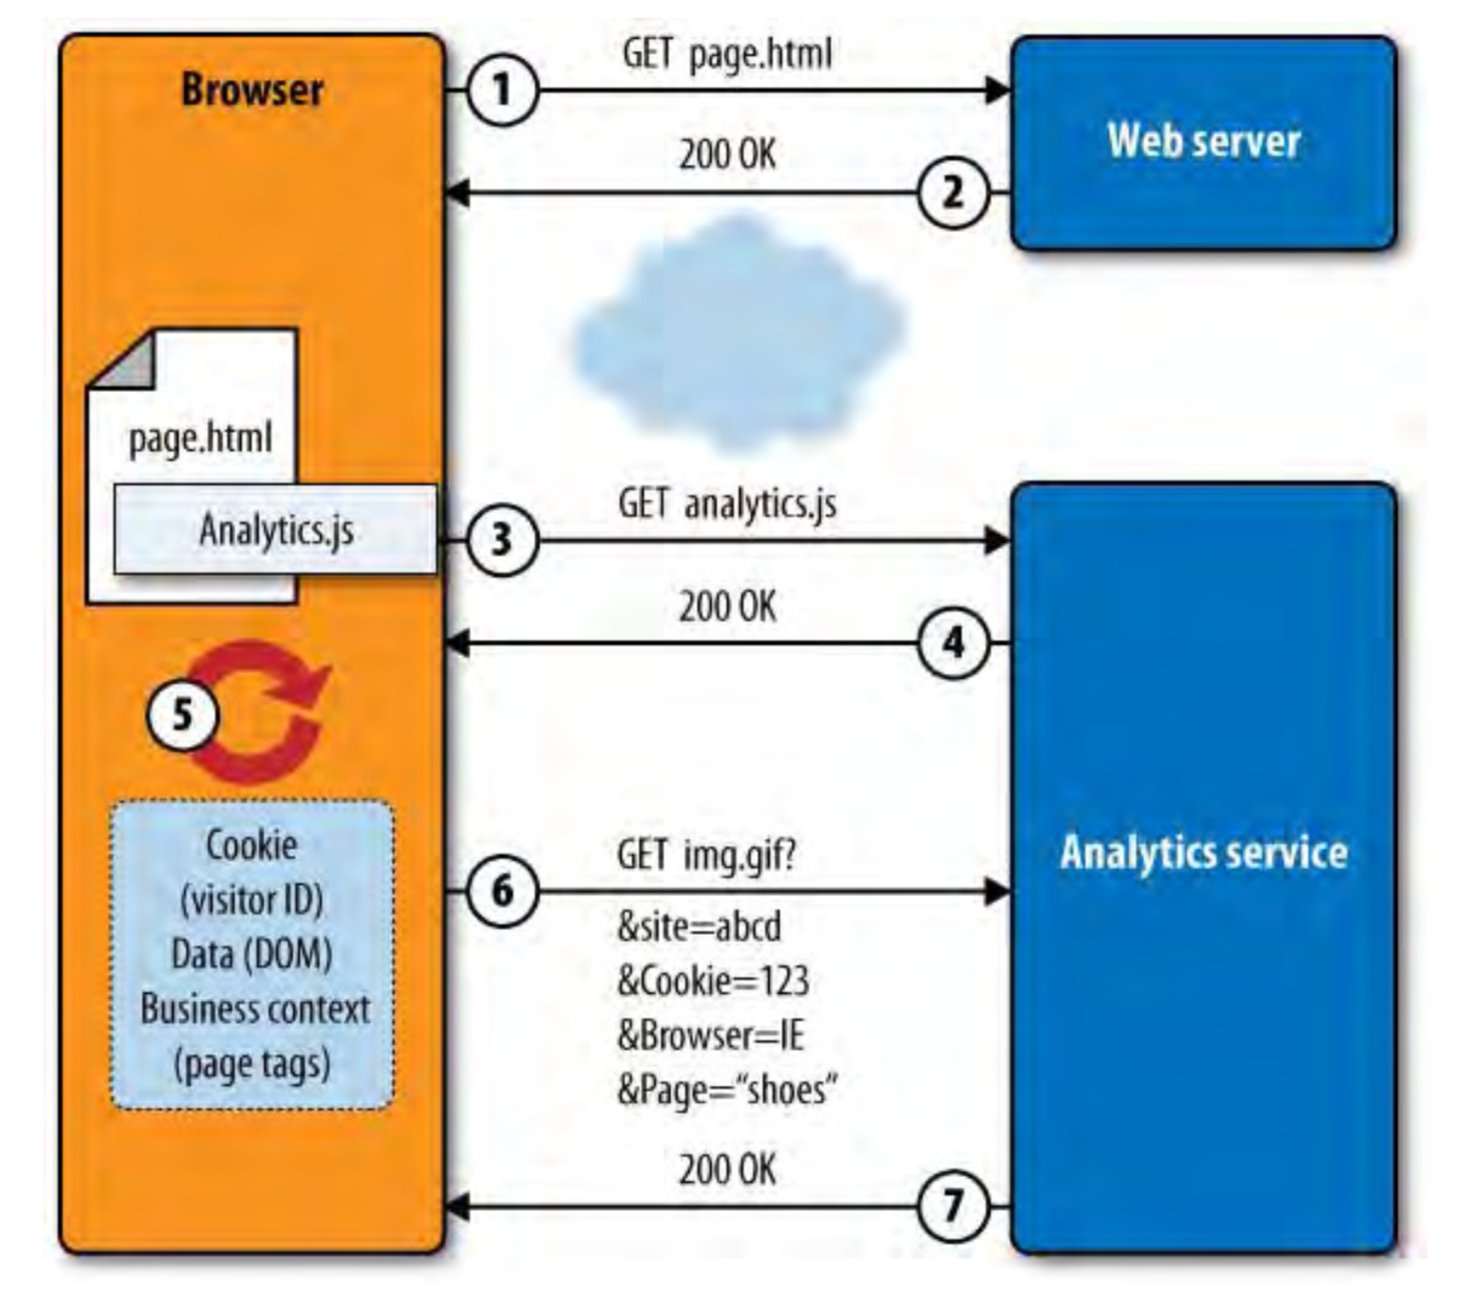
\includegraphics[width=0.5\textwidth]{page_tagging.png}
\caption{Page Tagging}
\label{img:page_tagging}
\end{center}
\end{figure}

The client (browser) requests a page from the web server (1, 2).
Within the HTML file an external JavaScript resource, the analytics code, is linked and received from the analytics server (3, 4).
The analytics script tracks and measures the user behaviour and eventually sends the data back to the analytics server (5, 6, 7).

The data collected can also be stored in cookies, which contain data beyond a session and enable the user to be identified, e.g. the next time he visits the page \cite{2019Kumar}.


The advantages and disadvantages of page tagging are as follows, starting with the pros (\cite{2009Waisberg}, \cite{2011Nakatani}, \cite{2011Marek}, \cite{2014Singal}, \cite{2015Zheng}):

%TODO again put all references on top ?

% [Pro]
\begin{itemize}
\item Every page visit is counted %cite 2009 Waisberg
\item The analytics service is outsourced, which includes the storage of the data, but also the data analysis and reporting %cite 2009 Waisberg
\item Page tagging is rather easy to implement and favourable when the analyst does not have access to the web server %cite 2011 Marek
\item Highly customizable: Everything that JavaScript enables to measure, collect, and track is available. This also includes information about the client such as screen size, device used or color depth. %cite 2011 Nakatani
\item Ability to track events and actions such as mouse clicks that do not send requests to the web server. This is especially important for single-page or progressive web applications that do not generate requests as often.  %cite 2011 Nakatani and 2015 Zheng
\item Mechanics of cookies provide identification of unique and repeat visitors %cite 2011 Nakatani
\item Real time reporting is possible %cite  2014 Singal 
\end{itemize}


% [Con]
Some drawbacks are mainly privacy concerns and the permission to collect data by the user,  that the analysis process relies on the use of JavaScript and cookies that can be disabled by the user \cite{2011Marek}, that every page that is supposed to collect data must contain the analytics script and due to the use of a third party analytics service it is pretty difficult to switch tools \cite{2014Singal}.



%TODO reference here that page tagging is used in RUM and RUM will be later explained in section X.


%TODO 2017 Hassler ch. 2 -> some good stuff there regarding pros and cons, see my notes




% TODO web beacons and packet sniffig ?:
% 2011 Marek
% 2011 Nakatani
% 2014 Singal



% ------------------------------------------


\subsection{Web Analytics Metrics}

%TODO go through the books again to have some nice introduction:
% why metrics, how are they useful, interpretation, etc.

[Introduction to Metrics]


% They should guide you on making important decisions for your business.


% [Business Metrics]

In this thesis, two kinds of metrics occur: Web Analyitcs metrics and Web Performance metrics.
Web Analytics metrics are metrics which reflect and quantify any business related aspect of the website.
I use the term "business" or "non-performance" metrics to draw a line between metrics mainly concerned with a websites performance and metrics reflecting other web analytics aspects.
I will use the terms "business", "non-performance" and "web analytics" metrics interchangeably.
Business metrics are not directly responsible to capture performance data such as loading speed of a website.
Performance metrics on the other hand are mainly related to website performance, for example site speed, as discussed in section X.


% [Relevance]

The selection of any kind of metrics and especially their relevance for the websites business enhancement is crucial.
It is important to measure what is important and relevant for the users and reaching business goals, while "each business has its own definitions of success". % cite 2009 Croll p 7,  https://developer.mozilla.org/en-US/docs/Learn/Performance/Measuring_performance
Hence, metrics are ideally tailored and custom to the website and they should track if "your business benefited in some way from their [the users] visits." % cite 2009 Croll p 15
Just as each website is unique and serves a different purpose, so should metrics be, which quantify the website.
As for each specific business question or use case, metrics can be made up, an unlimited amount of metrics exist.


% [Usable]

Metrics are only helpful when they are useful.
That implies that the collection and measurement of metrics should be consistent and their representation should be user-friendly and understandable. % cite https://developer.mozilla.org/en-US/docs/Learn/Performance/Measuring_performance
Kumar states that ideally, good metrics are uncomplex, relevant, timely, and instantly useful.  \\% cite 2012 Kumar


% [Interpretation]





% [Transition]

In this section, I will describe metrics which are more likely correlated and mapped to business topics, such as conversion or bounce rate.
In literature, a core corpus of web analytics metrics can be found and multiple ideas of structuring and categorizing those metrics exist.
The different possibilities of categorizations are discussed next.
Afterwards, one approach of categorization is then used to list a selection of common web analytics metrics.




% ------------------------------------


\subsubsection{Web Analytics Metrics Categorizations}


Categories help to better grasp and comprehend metrics, and they can provide structure and order.
Following are some examples of business metrics categorizations as they are presented in literature.

Peterson arguments from a marketing perspective and categorizes the metrics according to the customer life cycle, which includes the phases reach, acquisition, conversion, and retention. % cite 2004 Peterson

Metrics for measuring \textit{Reach} are for example number or percentage of new visitor.
\textit{Acquisition} contains metrics such as average number of visits per visitor or average pages viewed per visitor.
The category \textit{Conversion} includes metrics such as conversion or abandonment rates.
And the last category \textit{Retention} includes metrics such as the number of returning visitors.
This proposed categorization is highly customer-related and customer-centric and from a marketers perspective. 

%Reach:  - Overall Traffic Volumes,  Number of Visits
% Measuring Acquisition: - Percent New Visitors, - Average Number of Page Views per Visit
  
The Web Analytics Association defines three types and accordingly categories of metrics: \textit{Counts}, \textit{Ratios} and \textit{KPIs},% cite 2007 Burby
Where counts are metrics which are single numbers like the number of visits, ratios consist of counts divided by other counts, such as page views per visit.
KPIs are counts or ratios with a specific meaning and importance for the specific business.

Jansen defines four categories for web analytics metrics: % cite 2009 Jansen p.30
\textit{Site Usage}, which encompasses metrics such as demographics and system statistics, but also visitor length and type,
\textit{Referrers}, that are metrics describing the referring URL,
\textit{Site Content Analysis}, which includes metrics such as top pages or visitor paths, and
\textit{Quality Assurance} with metrics reflecting errors or other quality aspects of the measured system.

% Site usage: Internal Search Information
% Referrers: keyword Analysis	
	 
Croll arguments that all metrics answer at least one of four user-centric questions: \textit{What did they do?}, \textit{How did they do it?,} \textit{Why did they do it?}, and \textit{Could they do it?}. % cite 2009 Croll
Accordingly, the metrics are categorised by the question they answer.

Bekavac organizes the metric according to what they describe: \textit{Visits}, such as entry or exit page,
\textit{Visitors}, such as the metrics capturing new or returning visitors,
metrics such as page exit ratio or bounce rate which describe \textit{Visitor Engagement},
and metrics describing \textit{Conversions} as the conversion rate. % cite 2015 Bekavac

%visits: entry page, landing page, exit page, visit duration, referrer, ctr
%- For describing Visitors: repeat visitor, visits per visitor, recency, frequency
%- For describing Visitor engagement: page exit ratio, bounce rate

Hassler proposes a classification which is close and similar to the WAA proposed categorisation.
The metrics are ordered by their type: % cite 2017 Hassler
\textit{Counts} are absolute values like visitors or total sales,
\textit{Relations} put counts into relation for example as percentages, such as page views per visitor,
and \textit{Values} include non-numerical metrics such as referrer or search term.

Gessert et al.  propose a semantic categorization of metrics, they structure the metrics according to their meaning and their domain membership.
The categories are \textit{Performance}, which includes performance metrics such as Time to First Byte or First Input Delay (see section X.), \textit{User Engagement} metrics such as the session length or the bounce rate, \textit{Business KPIs} such as the cart size or the amount of transaction, but also conversion rates and revenue, and \textit{QA Metadata} which subsumes technical metrics like JS errors or the browser distribution.% cite 2020 Wolle https://www.youtube.com/watch?v=avPcOFzUa1Q&ab_channel=WolframWingerath

%- User Engagement: Session Length, First user interaction
% QA Metadata: Page views and sessions, Caching insights

%TODO add?
% 2004 Phippen
% 2020 Heinemann 4.1.4
%Metrics Categories for E-Shop:
%- Attraction
%- Acquisition
%- Retention
%- Umsatzleistung
%- Warenleistung
%- Ergebnisleitung

%- also customer life cycle

%TODO \ref{table:business_metrics_categorizations} somewhere...
\begin{table}[h]
	% \renewcommand{\arraystretch}{1.5} %TODO decide if spacing is needed
	\small
	\centering
	\begin{tabular}{ | l | l | }
	\hline
	Value-Driven
	& \{Counts, Ratios, KPIs\},  \\
	& \{Counts, Relations, Values\} \\
	\hline
	Semantic-Driven
	& \{Performance, User Engagement, Business KPIs, QA Metadata\},  \\
	& \{Site Usage, Referres, Site Content Analysis, Quality Assurance\} \\
	\hline
	Marketing-Driven
	& \{Reach, Acquisition, Conversion, Retention\}, \\
	& \{Visits, Visitors, Visitor Engagement, Conversions\} \\
	\hline
	\end{tabular}
	\medskip
	\caption{Possible categorizations of web analytics metrics}
	\label{table:business_metrics_categorizations}
\end{table}


% [Conclusion]

As described above, multiple categorizations of metrics are proposed in literature.
While some authors group the metrics by their type of value, e.g. if they count something or represent a ratio, others use a more semantic approach and group the metrics by their meaning, with some extreme examples by authors which group only through a marketing perspective.
% Orthogonal to semantic: "number" categorization: Count, ratio, ...

In the following, I will list some metrics and provide brief explanations, following the categorization of counts,ratios and values.
After that, i will take a look at metrics which are specific for performance.



%TODO add ?
% Customer Life Cycle and Pyramid
% 2004 Peterson
%Pyramid Model described the data itself and not metrics
%Metrics categorised by customer life cycle: Reach, Acquisition, Conversion, Retention

% 2008 Reese
%- Pyramidenmodell 




% ---------------------------------------------------------------


\subsubsection{Web Analytics Metrics Examples}


Table X provides web analytics metrics which are not directly concerned with performance.
The categories used to structure the metrics are \textit{Counts}, \textit{Ratios} and \textit{Non-Numerical Values}, like they are already defined by Hassler or WAA in the section above. % cite ?

%TODO even add this? already described above
% [Counts]
%Counts hold a value describing how many 
%Counts can be measured over time: last hour, month, from to, etc.
%Averages are possible
%Compare with Segmentation

% [Ratios]
%Ratios are a combination of numerical values.
%As Ratio or Percentage

% [Non-Numerical Values]
%Non-Numerical Values can not be reflected as a number.


\begin{center}
	\small
	\begin{longtable}{ | p{0.3\linewidth} | p{0.6\linewidth} | }
	
	\hline
	\multicolumn{2}{|c|}{ \cellcolor{lightgrey} Counts} \\
	\hline
	Hits & Represent amount of requests to the server.  \\ % 2004 Peterson
	\hline
	Visits or Sessions & Count how many users view the website \\ % 2004 Peterson
	\hline
	Session Length & How long the session endures \\ % 2007 Burby
	\hline
	Page Views & How often a page has been viewed \\ % 2004 Peterson
	\hline
	Single Page Visits & Sessions where one page has been viewed \\ % 2007 Burby
	\hline
	New / Unique / Repeat / Return Visitors & ... \\
	\hline
%	Time on Page & ... \\
	%\hline
%	Time between Visits & ... \\
%	\hline
	JS Errors & How many JS errors occured \\
	\hline
	Cart Size & ... \\
	\hline
	Conversions & ...  (business specific) \\
	\hline
	\textit{etc.} &  \\

	\hline
	\multicolumn{2}{|c|}{ \cellcolor{lightgrey} Ratios} \\
	\hline
	Conversion Rate & ... \\
	\hline
	Bounce Rate & ... \\
	\hline
	Abandonment Rate & ... \\
	\hline
	Page Views per Visitor & ... \\
	\hline
	New Visitors Percentage & ... \\
	\hline
	Visits per Visitor & ... \\
	\hline
	Page Exit Ratio & ... \\
	\hline
	Click Through Rate (CTR) & ... \\
	\hline
	\textit{etc.} & \\	
	
	\hline
	\multicolumn{2}{|c|}{ \cellcolor{lightgrey} Non-Numerical Values} \\
	\hline
	Demographics & ... \\	
	\hline
	Referrer & ... \\	
	\hline
	\textit{etc.} &  \\
	\hline
	
	\caption{Business Metrics Examples}
	\label{tab:businessmetrics}
	\end{longtable}
\end{center}


%\paragraph{Hits}
% 2004 Peterson
% 2017 Hassler


%\paragraph{Visits}
% 2004 Peterson
% 2007 Burby
% 2009 Waisberg
% 2017 Hassler

%\paragraph{Session Length}
% 2007 Burby


%\paragraph{Page Views}
% 2004 Peterson
% 2007 Burby
% 2009 Croll p. 74 Page View, first useful web analytics metric
% 2009 Waisberg
% 2015 Zheng
% 2017 Hassler


%\paragraph{Single Page Visits}
% 2007 Burby

%\paragraph{New Visitors}
% 2004 Peterson
% 2007 Burby

%\paragraph{Unique Visitors}
% 2004 Peterson
% 2007 Burby
% 2017 Hassler

%\paragraph{Repeat Visitors}
% 2007 Burby

%\paragraph{Return Visitor}
% 2007 Burby

%\paragraph{Time on Page}
%\paragraph{Time between Visits}

%\paragraph{JS Errors}

%\paragraph{Cart Size}
% 2009 Croll p 24 in site effectiveness

%\paragraph{Conversions}


% -------------- RATIOS --------------


%\paragraph{Bounce Rate}
% 2007 Burby
% 2009 Waisberg

%\paragraph{Conversion Rate}
% 2004 Peterson

% 2009 Croll
%- The percentage of visitors that your site converts to contributors, buyers, or users is the most important metric you can track

%\paragraph{Abandonment Rate}
% 2004 Peterson
% 2009 Croll

%\paragraph{Page Views per Visitor}
% 2007 Burby
% 2009 Waisberg

%\paragraph{New Visitors Percentage}
% 2009 Waisberg


%\paragraph{Visits per Visitor}

%\paragraph{Page Exit Ratio}
% 2007 Burby


%\paragraph{Click Through Rate (CTR)}
% 2004 Peterson
% 2007 Burby
% 2009 Croll



% % -------------- NON_NUMERICAL_VALUES --------------


%TODO find some more examples here

%\paragraph{Demographics}
%age, gender, browser, geography, ...

%\paragraph{Referrer}
% 2004 Peterson
% 2009 Croll



% --------------------------------------


% [Transition]

The table X provides a selection of common business metrics, following the proposed categorization of counts, ratios and non-numerical values and is not complete.
In the next section, I will discuss web performance and accordingly web performance metrics, which are designed to directly capture performance related data.


%TODO

[Transition to Web Performance]











%TODO even add this? outline can be made in beginning of next section
%As performance is directly connected to time, most of those performance metrics are measuring a timestamp.
%Some are also displaying a score. 
%This will be discussed.



%TODO should i show how to actual measure those metrics, like visits, hits, conversion rate etc ?


% Kessler 2012 -> dont have this digital...
% Erfolg messen und bewerten
 %Traffic:
%	 Page Impression / Page View
%	 Visit
%	 Visitor / Unique visitor
% Bounce rate
 %Conversion rate
 %CTR: Click-through-rate
 %Session length
 
 
 % 2016 Kollewe -> nicht digital
% Besucheranalyse: Wie viele Besucher?, Anzahl Besucher mit Mobilgerät, Demographische Daten (Geschlecht, Altersgruppe)
% Seitenanalyse: Was machen die Besucher im Shop?, Zielseite / Startseite: Erste Seite, die ein Besucher angeschaut hat, Ausstiegseite
% E-Commerce-Analyse: Transkations-daten aus Shop, Funnel-Analyse



% Terms and Definitions
\chapter{Web Performance}

[tbd]


[Last chapter]



[This chapter]

% In this chapter, I will cover measurement methods and discuss common performance metrics
% - This chapter should cover all relevant terms and definitions within web performance measurement
% How terms can be structured / taxonomy
% Ambiguity of definitions




[Relevance of this chapter for research question]





[Next chapter]





[Outline of this chapter]

%- Technical Background
%	   - Network
%	   - Front End: Navigation and CRP

%- Measuring Methods	

%- Metrics





% ---------------------------------------------------------------------------------------------------




\section{Introduction}
\label{chapter:web_performance}


%TODO make it clear the difference between web analytics and web performance
% web performance is also an analysis of the website, but not which users or how they interact with the website
% is about the website itself, how fast it is and how users perceive this performance

%TODO roter faden: What is web performance in web analytics context ?


% [Introduction]
% This chapter gives only a brief overview of the various aspects of web performance and appropriate sections below cover the topics in more detail.

% [Definitions]
As already described in chapter \ref{chapter:user_satisfaction}, web performance plays a role that cannot be neglected for user satisfaction and business success.
The cited studies show that increasing website performance also increases sales, or as Google states it: "Performance plays a major role in the success of any online venture".\footnote{\url{https://web.dev/why-speed-matters/} [03.06.2021]}

The MDN Web Docs identify multiple areas of web performance:\footnote{\url{https://developer.mozilla.org/en-US/docs/Learn/Performance/What_is_web_performance} [03.06.2021]}
\begin{itemize}
\item Reducing overall load time
\item Making the site usable as soon as possible
\item Smoothness and interactivity
\item Perceived performance
\item Performance measurements
\end{itemize}

%TODO add chapter references
\paragraph{Reducing load time}

In order to understand how load times emerge, the technical aspect of how websites are being loaded and presented to the user by the browser, needs to be comprehend.
This question is covered in chapter X.
%TODO do i really cover this ?

Concrete optimization steps and techniques to reduce load times are not focus of this thesis.


\paragraph{Usability and interactivity}

As I will describe in chapter X, there are several metrics available that attempt to reflect areas of performance such as load time, smoothness, and interactivity, and specific metrics are available as well as for differentiating between technical and user-perceived performance.


\paragraph{Performance perception}

The perception of performance is generally subjective.
As already seen in chapter \ref{chapter:user_satisfaction}, there are some quantifiable time intervals that correlate with human psychology regarding the received performance.
Table \ref{table:perception} contains "unofficial rule of thumb" for delay thresholds \cite{2013Grigorik}.


\begin{table}[h]
	\centering
	\begin{tabular}{| l | l | }
	\hline
	Delay & User Perception \\
	\hline
	0-100 ms & Instant \\
	100-300 ms & Small perceptible delay \\
	300-1000 ms & Machine is working \\
	> 1 s & Likely mental context switch \\
	> 10 s & Task is abandoned \\
	\hline
	\end{tabular}
	\label{table:perception}
	\caption{Rule of thumbs for delay}
\end{table}

If one interprets the numbers from the table, one can make the statement that it is desirable to keep loading times below one second.
Thresholds for certain performance metrics and the psychological rationale for setting them are discussed in chapter X. %TODO


% TODO add this?
% https://developer.mozilla.org/en-US/docs/Learn/Performance/why_web_performance
% financial aspect of downloading data and big websites



\paragraph{Performance measurements}
%TODO

There are several methods of measuring performance.
\textit{Synthetic monitoring }is discussed in chapter X.
\textit{Real User Monitoring} (RUM) is covered in chapter X.






% ---------------------------------------------------------------------------------------------------





\section{The Website Loading Process}


% [Introduction]

In order to understand web performance metrics and the methods to measure them, it is crucial to have a basic understanding of the technical aspect of the loading of a website into the browser.
This process includes establishing a connection between a client and a server, which will be discussed in section X, and the task of the browser to transform the received data from the server into a readable ready-to-use website, which will be discussed in section X.
%Always with performance in mind.


% [3 Entities: FE, BE, Network]

It is possible to divide the website loading process into three entities.
In his code talk 2016, Witt identifies three main areas of the website loading process: The Front End, the Back End, and the Network.  % cite 2016 Witt or just say this ??
The Front End is everything the user sees on the screen, client, UI, browser, sends requests to a back end, etc.
The Back End is the logic, server, also data base, handles requests and sends responses to a front end
Network is what connects clients and servers, FE and BE, infrastructure element composed of routers, cables, wireless connections etc.

The main steps can be divided into networking, that is, establishing a connection with DNS etc., backend processing, e.g. data base queries etc., and the rendering in the front end, as seen in image X.
The last part of this process is when browser receives finally the HTML / Document. 
How the browser transfers the HTML into an interactive website is part of the next section.



\begin{figure}[h!]
\begin{center}
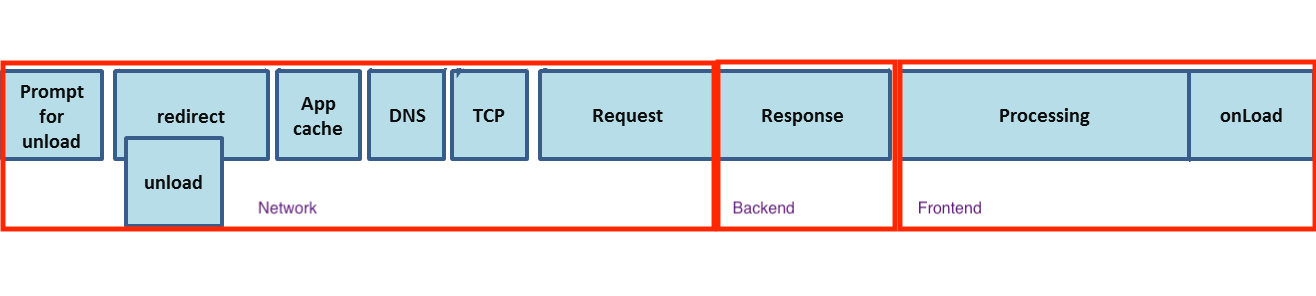
\includegraphics[width=0.8\textwidth]{timing_overview_blanco2.png}
\caption{Timing Overview}
\label{img:timing_overview}
\end{center}
\end{figure}
%TODO change image: make it clean


- BE is not discussed (server time, data base, etc.)
- Section X is about Network
- Section X is about Front end: how browser works, crp, 
- How to optimise websites is not part of this thesis




% [Performance]

Focus and perspective is performance, like in overall thesis.
Also when explaining the technical background, I will keep the aspect of performance in mind.

Once I discussed the processes in the network and the front end, I will move on to the question of how to measure the performance of those processes, and which metrics are available to quantify the performance.


%TODO should I talk about metrics already in this section ?


% --------------------------------------------------------------------------------------------
% --------------------------------------------------------------------------------------------


\subsection{The Website Loading Process in the Network}

[tbd]

The network is... Starting from hardware, ISP, routers, switches etc and the cables connecting them.
But also communication protocols such as the Internet protocol suite.

Regarding performance, latency and bandwidth come into mind, and we will see that latency has a bigger impact on performance than bandwidth in section X.

After discussing this issue, i will continue by describing the process or navigation steps which happen once the user enters a URL into the browser, up until he sees pixels on his screen and can use the website.


% --------------------------------------------------------------------------------------------


\subsubsection{Latency and Bandwidth}

There are two important attributes when discussing network performance: Latency and Bandwidth.
The important thing to say here is that Latency is bottleneck for performance, and not bandwidth.


% [Bandwidth]

Bandwidth is the "maximum throughput of a logical or physical communication path". %cite 2013 Grigorik
In other words, bandwidth describes the amount of data which can be sent in parallel from one node in a network to another. 
Physical communication paths are most likely cables such as metal wires or fiber-optic cables, where fiber-optic cables have less signal loss, and lower lifetime maintenance costs.
With methods such as wavelength-division multiplexing (WDM), it is possible to transmit up to 70 Tbit/s over a fiber-optic connection.  %cite 2013 Grigorik
This high technology stuff is only used in the backbone infrastructure, e.g. for connecting Europe with America.
For the end user, bandwidth is much lower, and the average was in late 2015 just 5.1 Mbps %cite 2013 Grigorik
A high bandwidth is useful for bulk or large data transfer such as streaming of video or audio.
But for loading a website,or any browser activity that depends on many requests that fetch data from many different locations around the globe, the performance bottleneck is latency. % cite 2013 Grigorik


% [Latency]

Latency is "the time from the source sending a packet to the destination receiving it".  % cite 2013 Grigorik
Latency is measured in seconds and can be the time spent for one-way, or more common, how long it takes for the transmitted data package for the round-trip time (RTT), from source to destination and back.
In other words, latency "describes the amount of delay on a network or Internet connection". % cite https://developer.mozilla.org/en-US/docs/Web/Performance/Understanding_latency
For the very first request when establishing a connection, latency is longer due to protocols such as DNS lookup, TCP and TLS handshakes.
Those will be discussed in section X. % cite https://developer.mozilla.org/en-US/docs/Web/Performance/Understanding_latency


% [Experiment]

To get an idea about how the two aspects, bandwidth and latency, impact web performance,  Mike Belshe launched a study. % cite https://docs.google.com/a/chromium.org/viewer?a=v&pid=sites&srcid=Y2hyb21pdW0ub3JnfGRldnxneDoxMzcyOWI1N2I4YzI3NzE2
Once setup has a fixed latency and bandwidth is variable, and vice versa.
He and compared the performance of the two experiments using the Page Load Time metric. (cf. X for this metric)


\begin{figure}[h!]
\begin{center}
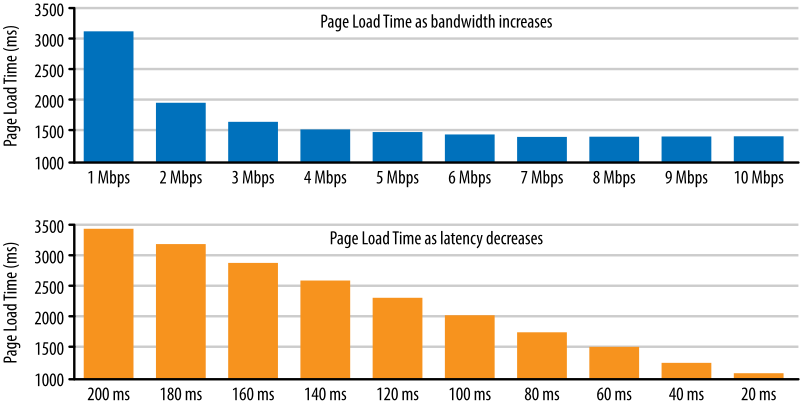
\includegraphics[width=0.8\textwidth]{latency.png}
\caption{Latency vs Bandwidth}
\label{img:latency}
\end{center}
\end{figure}


We can see that the impact of bandwidth is trivial: if the available bandwidth is doubled, e.g. from 5 to 10 Mbps, there is no change in performance load time.
For Latency on the other hand, the picture is different: If the latency can be decreased by half, e.g. from 120 ms to 60 ms, the page load time also sinkt um die hälfte.
Or as Belshe states it, "[reducing] cross-atlantic RTTs from 150ms to 100ms [...] would have a larger effect on the speed of the internet than increasing a user's bandwidth from 3.9Mbps to 10Mbps or even 1Gbps." % cite https://docs.google.com/a/chromium.org/viewer?a=v&pid=sites&srcid=Y2hyb21pdW0ub3JnfGRldnxneDoxMzcyOWI1N2I4YzI3NzE2

This observations can be explained with the many short, small connections and requests are made when browsing websites and the contrary underlying structure of the communication protocols, which are "optimized for long-lived connections and bulk data transfers. " %cite 2013 Grigorik ch 10
But just simply decreasing the latency is not straightforward: The speed of data transfer is already at a 2/3 of light, but the physical constraint is the limiting factor, e.g. there is a minimum distance between London and New York which can not be further "optimized". % cite 2013 Grigorik Ch 1


% [Mobile]

Another aspect of latency is that for wireless connections and therefore mobile devices, latency is even higher, "making networking optimization a critical priority for the mobile web." % cite 2013 Grigork Ch 1
This is due to the infrastructure of mobile nets, latency is high for mobile users. cf.  Why are mobile latencies so high? in Grigorik % cite https://www.igvita.com/slides/2013/fluent-perfcourse.pdf


% [Transition]

As latency is a important factor, what happens on the front end is still important.
And again for this thesis metrics measuring performance in the front end are the focus.

Before i will discuss what happens in the browser once the website data arrived, i will briefly describe the preceding steps of establishing a connection between the browser (client) and the server, which can be considered to be still a part of the network.




%TODO add this ?
% Use other techniques such as CDNs, caching, pre-fetching, etc % 2013 Grigorik
% CDN: Help against this issue. Put stuff close to client % 2013 Grigorik
% Some direct implications for performance measurement ?
% Understanding Latency https://developer.mozilla.org/en-US/docs/Web/Performance/Understanding_latency
% Network throttling: Emulate download speed, upload speed, and minimum latency



% --------------------------------------------------------------------------------------------


\subsubsection{Network Navigation Steps}

[tbd]

I will explain briefly the main navigation steps: It begins when the user is submitting a URL in the browser and ends when he received website data.

"To start, it is important to recognize that every HTTP request is composed of a number of separate stages (Figure 10-3): DNS resolution, TCP connection handshake, TLS negotiation (if required), dispatch of the HTTP request, followed by content download." % cite Grigorik 2013


%TODO add this ?
% Understanding Latency https://developer.mozilla.org/en-US/docs/Web/Performance/Understanding_latency
%Network Timings:
%- Blocked: When a request is in queue
%- Blocking happens when there are too many simultaneous connections to single server over HTTP



% ----------------------------------


\paragraph{DNS Lookup}

When the requested resource can not be loaded from the browsers cache, the first step to establish a connection is a DNS Lookup (or DNS Resolution).

This step is about translate URL to IP address.
Must be done for each unknown URL, e.g. when linked images within a website are from different server, for each unique URL DNS Lookup has to be done.
The mapping of URL to IP can be cached by browser, which makes repeated views faster. % cite https://developer.mozilla.org/en-US/docs/Web/Performance/How_browsers_work

Avg. time is 20 and 120 ms % https://www.keycdn.com/support/reduce-dns-lookups

%Metric?
%Can be considered a performance metric, see section X.


% ----------------------------------


\paragraph{TCP Handshake}

Once a connection between a client and a server is established, the TCP 3-way-Handshake comes into play.

The goal of TCP is to establish a reliable connection within an unreliable network.
TCP  "guaranteed that all bytes sent will be identical with bytes received and that they will arrive in the same order to the client. " %cite 2013 Grigorik
Regarding performance, the handshake adds two more round trips, which is bad for performance as we have seen because of latency.

Many algorithms and techniques to get optimal data transfer and also avoid congestion are existing, such as Slow-Start.
Slow-Start is an algorithm that determines the maximum bandwidth that can be used by gradually increasing the amount of data sent.
Slow start prevents that the full capacity of the network is being used from the beginning, which in performance terms adds again more round trips and latency. %cite 2013 Grigorik

For a detailed discussion cf "Building Blocks of TCP" in 2013 Grigorik % cite https://hpbn.co/building-blocks-of-tcp/

%TODO once i know which metric add it here ?
%A performance metric reflecting the time spent for establishing a TCP connection is X, see section X.




% ----------------------------------


\paragraph{TLS Negotiation}

TLS is another protocol which has the goal to establish a secure connection in terms of data encryption.
Data transmitted over the network has to be encrypted so that aussenstehende can not read or manipulate the data.
For encryption,  a cipher to be used needs to be established, which will be shared between client and server during the TLS Negotiation. % cite https://developer.mozilla.org/en-US/docs/Web/Performance/How_browsers_work

TLS again adds more round trips which is bad for performance.

for a detailed discussion see Transport Layer Security (TLS) in 2013 Grigorik % https://hpbn.co/transport-layer-security-tls/

%TODO once i know which metric add it here?
%A performance metric reflecting the time spent for a TLS negotiating is blabla in section X.


% ----------------------------------


\paragraph{HTTP Request and Response}

Now that a secure connection is established, the client fetches the first resources via HTTP GET request.
Most often, the server will respond by sending back the index.html file, which then can be used by the browser to build the website. % cite https://developer.mozilla.org/en-US/docs/Web/Performance/How_browsers_work

The time when this first response containing the first byte for building the web site is reflected in the metric TTFB which is discussed in section X.


% [Connection vs Request]

Usually, many more resources are requested by the browser to complete the build of the web site.
As of today, the median value is about 70 requests per web site. % footnote https://httparchive.org/reports/state-of-the-web#reqTotal

A request is not the same as a connection.
Once the connection is established via the above described procedures such as DNS lookup, TCP and TLS handshakes, multiple requests can be transmitted over the same connection.
Usually, the number of requests is much higher than the number of connections to load a website, as the browser persist connections, keep them open for multiple requests.
Median connections for a web site today is about 13. % footnoe https://httparchive.org/reports/state-of-the-web#tcp
Modern browsers like Chrome enable up to six open connections in parallel. % cite 2014 Hogan



% [Transition to CRP]

At this point, the browser has received the first data about the web site and he can start with rendering the page.
How this exactly happens, is explained in the next section.




% --------------------------------------------------------------------------------------------
% --------------------------------------------------------------------------------------------



\subsection{The Website Loading Process in the Frontend: Critical Rendering Path}

This section explains what happens after the first bytes of the web sites arrived in the browser.
The following processes are typically subsumed under the term \textit{Critical Rendering Path} (CRP).
The CRP is the last part of the navigation process as seen in image X.


% [Critical]

The CRP is the minimum steps that the browser has to take from the moment it receives the first byte of HTML to the moment that it renders pixels on the screen for the first time.

The rendering is critical as it is the very first render, the first visible content the user will see on the screen.
The resources that are needed for the first render of the page delay the first render of the page are considered to be critical.
Without the critical resources, the browser can not display content on the screen.
An example of a critical resource is the first HTML file the browser receives, as without it, nothing is visible on the screen.
Non-critical resources on the other hand will not stop the browser from displaying the first content on the screen. % cite https://blog.logrocket.com/how-css-works-parsing-painting-css-in-the-critical-rendering-path-b3ee290762d3/


% https://gtmetrix.com/blog/how-to-eliminate-render-blocking-resources/
%- Non-critical resources are those that provide contributions to secondary/tertiary functionality or styling for the content on your page, e.g., a calendar widget on the sidebar below-the-fold.


% https://blog.logrocket.com/how-css-works-parsing-painting-css-in-the-critical-rendering-path-b3ee290762d3/
%- Any CSS that is not necessary for the first load can be considered “non-critical”



% [CRP Steps]

There are a sequence of steps the browser goes through to render the page.
The basic idea is to convert HTML, CSS and JS to actual pixels on the screen.

Image X visualizes the flow of the CRP:
Once the HTML is received, the browser starts with parsing the HTML and translate it into the DOM.
The content of the CSS files will be parsed to the CSSOM.
JavaScript needs to be fetched and executed.
Once DOM and CSSOM are available, the Render Tree is being created.
When the Render Tree is available, Layout is happening.
Finally, pixels can be printed on the screen.
% cite https://developer.mozilla.org/en-US/docs/Web/Performance/Critical_rendering_path

In the following, the individual steps will be discussed in more detail.


\begin{figure}[h!]
\begin{center}
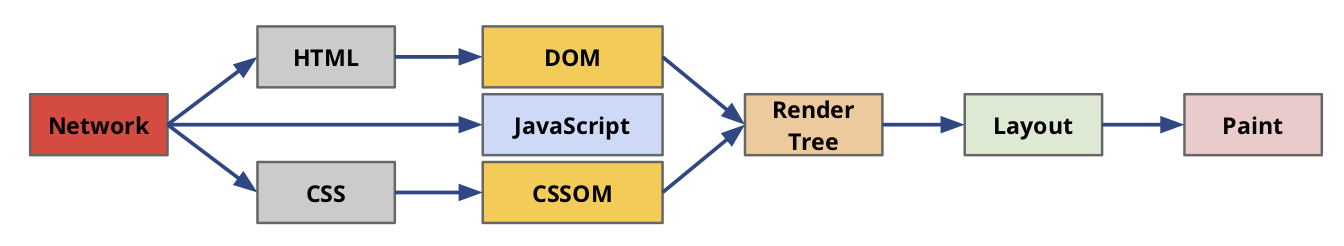
\includegraphics[width=0.7\textwidth]{crp.png}
\caption{Critical Rendering Path}
\label{img:crp}
\end{center}
\end{figure}



% [Single Thread]
%TODO do i need this ?
% How Browsers Work https://developer.mozilla.org/en-US/docs/Web/Performance/How_browsers_work
%- This is somewhat the bottleneck or the technical state of the browser
%- Browser is single threaded
%- Still: Enable smooth interaction: scrolling, responsive to touch, etc.
%- Render time is key
%- Goal: Main thread can complete all the work and still is available to handle user interaction
%-> Improvement: Understand single thread concept of browser and minimize main threads responsibilities
%-> Should lead to: rendering is fast and smooth and responses to interactions are immediate



\paragraph{DOM Construction from HTML}

% [Introduction, Standard]

Once the browser received the first bytes of the HTML file, it starts to parse it into the \textit{Document Object Model} (DOM).
The DOM construction is the first step the browser performs when receiving data.
The DOM is a tree structure and internal representation of the HTML for the browser. % cite https://developer.mozilla.org/en-US/docs/Web/Performance/How_browsers_work
The general parsing process consists of translating from bytes to characters, to tokens, to nodes and finally to the object model.% cite https://developers.google.com/web/fundamentals/performance/critical-rendering-path/constructing-the-object-model
The specification of the DOM is maintained by the WHATWG living standard. % footnote https://dom.spec.whatwg.org/

% The Parsing of the HTML into the DOM is defined in the HTML standard % footnote https://html.spec.whatwg.org/multipage/parsing.html#parsing


% [Render Blocking]

The DOM tree contains information about the content of the document, but not its style.
The styling is defined in the CSS.
Once HTML and CSS are transmitted and processed by the browser, the \textit{Render Tree} can be created, which reflects the actual information and its styling the browser can display.
Within this context, it is possible to categorise resources into render blocking and non-render blocking.
A render blocking resource is a resource that prevents the browser from rendering content to the screen.
HTML and CSS are render blocking resources, as the parsing process of those files blocks the browser of displaying the page to the screen.% cite https://developers.google.com/web/fundamentals/performance/critical-rendering-path/render-blocking-css

% CSS parsing and render tree construction will be discussed below.


% [Incrementally]

As soon as the first data packages of HTML arrive at the browser, the parsing process starts. %cite How Browsers Work https://developer.mozilla.org/en-US/docs/Web/Performance/How_browsers_work
The DOM is created incrementally,  this means that the browser can begin to process the HTML before all of its content is transmitted over the network.


% [Resources]

Usually, within the HTML, external resources are linked which are necessary for the website to be complete, such as CSS or JavaScript.
While parsing the HTML incrementally, eventually a reference to such an external resource will be encountered.
How the external resources CSS and JavaScript are being handled by the browser is discussed below.


%TODO add this?

% How Browsers Work https://developer.mozilla.org/en-US/docs/Web/Performance/How_browsers_work
%- DOM is also exposed, and can be manipulated through various APIs in JavaScript 
%Optimisation: Preload scanner:
%- This process occupies main thread while browser is building DOM Tree
%- parse through the content available and request high priority resources like CSS, JavaScript, and web fonts.
%- will retrieve resources in the background so that by the time the main HTML parser reaches requested assets, they may possibly already be in flight, or have been downloaded




% ------------------------------------------------------------


\paragraph{CSSOM Construction from CSS}


% [Introduction]

The CSS resource contains all information about the styling of the page.
As with the HTML,CSS is converted from bytes to characters, to tokens, to nodes, and finally to the \textit{CSS Object Model} (CSSOM). % cite https://developers.google.com/web/fundamentals/performance/critical-rendering-path/constructing-the-object-model
CSSOM construction is usually very fast . % cite % How Browsers Work https://developer.mozilla.org/en-US/docs/Web/Performance/How_browsers_work
CSSOM is standardized here % footnote https://drafts.csswg.org/cssom/

% The DOM and and CSSOM are separated structures and not yet connected.
% The Render Tree reflects the combination of the two models and will be discussed below.
% Creation of CSSOM happens after DOM is completed. % https://developer.mozilla.org/en-US/docs/Web/Performance/Critical_rendering_path



% [Cascading, Not incrementally]

As opposed to the HTML parsing process, CSS can not be translated to the CSSOM incrementally.
Cause it the cascading nature of style sheets, which has the potential that the styling rules defined at the top of the file may be overridden by rules defined at the very end of the CSS file.
A partial CSSOM is therefore not possible.
Hence the browser needs the entire CSS file before he can create the CSSOM.
%cite  https://developer.mozilla.org/en-US/docs/Web/Performance/Critical_rendering_path


% [Not Parser Blocking]

As soon as the parser encounters a reference to an external style sheet such as

%TODO add caption={} ?
\begin{lstlisting}[language=html, numbers=none]
<link rel="stylesheet" href="styles.css">
\end{lstlisting}

it requests the resource and continues with parsing the HTML.
CSS is not a parser blocking resource.
When the CSS arrived at the browser, the CSSOM construction starts.
%cite  https://blog.logrocket.com/how-browser-rendering-works-behind-the-scenes-6782b0e8fb10/


%TODO add FOUC ?

% https://blog.logrocket.com/how-css-works-parsing-painting-css-in-the-critical-rendering-path-b3ee290762d3/
% - If it just went ahead and rendered to pixels without waiting for the CSSOM we’d see a flash of unstyled content (ugly!) for a moment while the CSSOM was parsing.



% [Render Blocking]

While CSSOM creation is not parser blocking, it is render blocking.
The browser blocks the page rendering until it received and parsed all of the CSS.
Rendering content to the screen is only possible when CSSOM and therefore CSS is available. % cite https://developers.google.com/web/fundamentals/performance/critical-rendering-path/render-blocking-css


% [When finished]

Once the DOM and CSSOM are created, they can be merged together into the render tree, which will be layout and painted to the screen.
Before I describe this process, I will discuss how JavaScript is being handled.


% [Optimization]

%TODO add this: optimization
%- You want to get CSS down to the user as quick as possible:
	%- Inlining styles
	%- Load not needed styles later
%- Optimization: use media queries
%- Better to add styles in single file
%- FOUC: Flash of Unstyled Content: If unstyled content is visible on the screen


% https://developers.google.com/web/fundamentals/performance/critical-rendering-path/render-blocking-css
%Media types and media queries allow us to mark some CSS resources as non-render blocking.


%TODO add this? Lighthouse what is render blocking https://web.dev/render-blocking-resources/
%Lighthouse flags resources as render blocking when:
%A <link rel="stylesheet"> tag that:
%Does not have a disabled attribute. When this attribute is present, the browser does not download the stylesheet.
%Does not have a media attribute that matches the user's device.





% ------------------------------------------------------------



\paragraph{JavaScript in the Critical Rendering Path}


% [Introduction, Parser and Render Blocking]

JavaScript (JS) resources add functionality and interactivity to a web site.
When the browser encounters a script tag such as

%TODO add caption={} ?
\begin{lstlisting}[language=html, numbers=none]
<script src="myScript.js"></script>
\end{lstlisting}

it will stop its current task of parsing, fetch immediately the resource and execute its content, and only then proceed with the creation of the DOM. % cite % Grigorik Conference Talk https://www.youtube.com/watch?v=PkOBnYxqj3k&ab_channel=IlyaGrigorik
See image X.

JS can manipulate and query the DOM tree and directly change the HTML file.
As the HTML file is the input stream for the parser,  the parser stops until the JS is downloaded and executed. % cite https://developer.mozilla.org/en-US/docs/Web/Performance/Critical_rendering_path
Hence JS is parser blocking.
JS fetching and execution stops the parsing of the HTML and the construction of the DOM.
Only after the script finished execution, HTML parsing will continue.

Implicitly, because JS execution blocks DOM creation, and HTML processing itself is render blocking, JS is also render blocking. % cite Grigorik Conference Talk https://www.youtube.com/watch?v=PkOBnYxqj3k&ab_channel=IlyaGrigorik


The behaviour is the same for an external references JS file and a script directly added within in the HTML.


%TODO add this?

% This means that excessive scripts can be a significant bottleneck % How Browsers Work https://developer.mozilla.org/en-US/docs/Web/Performance/How_browsers_work

% https://blog.logrocket.com/how-browser-rendering-works-behind-the-scenes-6782b0e8fb10/
% - If the network is slow, and it takes thousands of milliseconds to fetch app.js, the DOM construction will be halted for the thousands of milliseconds as well

% https://blog.logrocket.com/5-tricks-to-eliminate-render-blocking-resources/
%- You can remove them from the critical rendering path by placing the <script> tags right before the closing </body> tag instead of the <head> section.
%-In this case, they only begin to download after the entire HTML has been downloaded.

% https://developer.mozilla.org/en-US/docs/Web/Performance/How_browsers_work
%- Though the browser's preload scanner hastens this process.


% [Blocked by CSS]

As JS can also manipulate the styling of the page, its execution is blocked until the CSSOM is available.
This means that the execution of the JS is on hold until the CSSOM is ready.
To summarize, while JS blocks the parsing of the HTML to the DOM, JS execution itself is blocked by the creation of the CSSOM.
CSSOM blocks JS, and JS blocks DOM construction. %cite 2013 Grigorik ch 10

Several attributes on the script tag can change the behaviour of the browser.
\textit{Async} and \textit{defer} are options to counter the blocking nature of the script tag.
They will be discussed now.\\



% [async attribute]

With the async (asynchronous) attribute, the browser downloads the JS in the background while continuing with the parsing of the HTML.
The parsing is not blocked and the browser can continue with his task. 
As soon as the JS is downloaded and available,  it is parser blocking: the browser stops the parsing and executes the JS.%cite https://developer.mozilla.org/en-US/docs/Web/HTML/Element/script

The order of all the async scripts within the document is not maintained any more.
Whenever a script is downloaded and available, it will be executed.
It does not matter if an async script was included at the top or bottom of the HTML document. % cite https://blog.logrocket.com/5-tricks-to-eliminate-render-blocking-resources/



% https://blog.logrocket.com/5-tricks-to-eliminate-render-blocking-resources/
%- The async attribute is recommended for independent third-party scripts, such as ads, trackers, and analytics scripts. For example, Google Analytics recommends adding the async attribute to support asynchronous loading in modern browsers.


% [defer attribute]

Like with async, scripts with the defer attribute enable the browser to download the script in parallel while continuing with the parsing of the HTML.
Contrary to async, defer scripts will only be executed after the parsing of the page is complete and the DOM tree is fully constructed,  and the order of the scripts will be maintained.  %cite  https://blog.logrocket.com/5-tricks-to-eliminate-render-blocking-resources/


\begin{figure}[h!]
\begin{center}
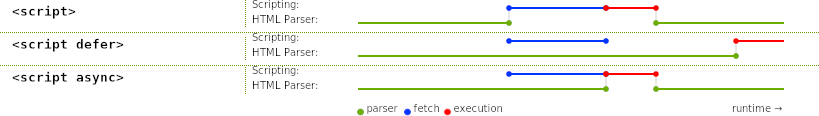
\includegraphics[width=0.8\textwidth]{scripts.png}
\caption{Scripts}
\label{img:latency}
\end{center}
\end{figure}


The async and defer attributes not applicable on inline scripts.
The HTML standard states that  "scripts may specify defer or async, but must not specify either unless the src attribute is present. " % \footnote https://html.spec.whatwg.org/multipage/scripting.html#attr-script-async
As inline scripts do not contain a src attribute, as the source of the script is within the script tags and not external, the async and defer attributes are not applicable.


% https://blog.logrocket.com/5-tricks-to-eliminate-render-blocking-resources/
%- The defer attribute is recommended for scripts that need the DOM, but you want to begin to download them before the document loads, without making them a render blocking resource.
%- You should also use defer rather than async if the document order is important — for instance, when consecutive scripts depend on each other.



% [Transition] ??





% [More stuff]

%TODO add this? preload scanner
% https://developer.mozilla.org/en-US/docs/Web/Performance/How_browsers_work
%- Though the browser's preload scanner hastens this process.

% Grigorik Conference Talk https://www.youtube.com/watch?v=PkOBnYxqj3k&ab_channel=IlyaGrigorik
% And slides https://www.igvita.com/slides/2013/fluent-perfcourse.pdf
%- Asynchronous pattern:
	%- Not the same as async/defer tag
	%- Will fetch JS asynchronously
	%- Uses IIFE which creates a new script tag in the HTML with attribute async
	%see chapter X how Google Analytics is doing this.


%TODO add this? https://web.dev/render-blocking-resources/
%Lighthouse flags resources as render blocking when:
%A <script> tag that:
%Is in the <head> of the document.
%Does not have a defer attribute.
%Does not have an async attribute.


%TODO add this? resource hints
% https://blog.logrocket.com/using-resource-hints-to-optimize-performance/





% ------------------------------------------------------------




\paragraph{Building the Render Tree}


As already described above, HTML and CSS are both render blocking, as they prohibit the rendering of the page.
Rendering can happen once the \textit{Render Tree} is available.
The render tree is the combination of the DOM and CSSOM and captures all visible content with its styles which will be displayed on the screen.
If an element has a CSS property such as \verb|display: none;| it will not occur in the render tree. % cite https://developers.google.com/web/fundamentals/performance/critical-rendering-path/render-tree-construction

The computed render tree is then used to layout the content to the page.


%TODO add this ? Check again when chapter about WPT metrics is done
% 2014 Hogan https://designingforperformance.com/
%Chapter 2
%- Start Render Metric in WPT




% ------------------------------------------------------------


\paragraph{Layout}


In the layout process, the position and size of the nodes from the render tree are calculated.
New layout calculations or reflows are triggered as soon as the screen area changes, e.g. by device rotation or window resizing, or on modifications of the DOM and render tree. % cite How Browsers Work https://developer.mozilla.org/en-US/docs/Web/Performance/How_browsers_work

Once the layout is resolved, the browser continues with painting pixels on the screen.


%TODO add viewport? The projection area is dependent and defined by the viewport

% https://developer.mozilla.org/en-US/docs/Web/Performance/Critical_rendering_path
%- The viewport meta tag defines the width of the layout viewport, impacting the layout.
%- Without it, the browser uses the default viewport width, which on by-default full screen browsers is generally 960px. On by-default full screen browsers, like your phone's browser, by setting <meta name="viewport" content="width=device-width"



% ------------------------------------------------------------


\paragraph{Paint}

Finally, the browser can paint the content on the screen.
If some content changes, browsers are optimized to only repaint areas on the screen affected.  %cite  https://developer.mozilla.org/en-US/docs/Web/Performance/Critical_rendering_path



%TODO add metrics ?
% How Browsers Work https://developer.mozilla.org/en-US/docs/Web/Performance/How_browsers_work
%-> First Meaningful Paint
%- Time to Interactive


%TODO add above the fold?
% https://gtmetrix.com/blog/how-to-eliminate-render-blocking-resources/
%- Above the fold: “Above-the-Fold” refers to the area that the visitor normally sees on a website before scrolling down to see the rest of the content. 


%TODO add performance question?
% https://blog.logrocket.com/how-css-works-parsing-painting-css-in-the-critical-rendering-path-b3ee290762d3/
%- Paint: It’s important to remember that some CSS properties can have a larger impact on the page weight than others (for example, a radial-gradient is much more complex to paint than a simple color).




% ------------------------------------------------------------


%TODO add this ?

% [Continuos Loop, 60 frames per second]

% [Compositing ?]


% ------------------------------------------------------------


\subsection{Technical Background Conclusion}

[tbd]

Network, BE and FE.
Network: Latency and Bandwidth, Navigation steps
FE: CRP

[Link to next section]
Why was this section important for research question?
How is it connected to measurement methods and metrics?


% We could see that performance Metrics are directly derived from this process ??
% Measurement methods will be discussed next
% After that, i will talk about which metrics are available to capture performance data



%TODO add ?
% give some links and references to optimization

% [Optimizations]

% Grigorik Conference Talk https://www.youtube.com/watch?v=PkOBnYxqj3k&ab_channel=IlyaGrigorik
% And slides https://www.igvita.com/slides/2013/fluent-perfcourse.pdf
%- Optimize the critical rendering path!
%-> styles at the top, scripts at the bottom best practice
% - Different browsers implement different logic for when, and in which order, the individual resource requests are dispatched. As a result, the performance of the application will vary from browser to browser. 2013 Grigorik ch 10



% 2014 Hogan https://designingforperformance.com/
%- Optimizations of CRP:
%- media types and queries on css resources, which makes them non-blocking
%- Load JS efficient
%- Priotize requests for above the fold
%- etc. % Do i need to explain this ??
%Chapter 4:
%CSS and JavaScript Loading:
%- Rules:
%- Load CSS in head
%- CSS blocks rendering
%- Load JS at bottom of the page
%- Load Async
%- JS blocks DOM construction, because browser knows that content from script tag may change Render Tree
%- async tag will execute script once its ready, but order is not berücksichtigt
%- Anything that loads late and changes UI can cause layout shifts
%- 3rd party scripts: Need additional DNS lookup, should not be single point of failure

% https://developer.mozilla.org/en-US/docs/Web/Performance/Critical_rendering_path
%- Optimizing for CRP

% https://medium.com/@luisvieira_gmr/understanding-the-critical-rendering-path-rendering-pages-in-1-second-735c6e45b47a
%- Optimizing

% Grigorik Conference Talk https://www.youtube.com/watch?v=PkOBnYxqj3k&ab_channel=IlyaGrigorik
% And slides https://www.igvita.com/slides/2013/fluent-perfcourse.pdf
%- Async all the things! nice image about async attribute
%- Optimizing DOM:
	%- Minify HTML
	%- Compression
	%- Cache in Browser
%- Unblocking CSS:
	%- Media queries: for responsive design
	%-> Move media queries to separate file
	%- <link rel="stylesheet" href="style-print.css" media="print">
	%-> Will not block rendering
%- Optimizing JS:
	%- Minify, compress, cache
	%- JS is parser blocking
	%- Script tag blocks DOM construction
	%- For external JS, browser waits until JS is fetched and executed
	%- CSS blocks rendering and JS execution
	%- Load and execute script after page is loaded
	%- Page is loaded: Browser fires onload event
	%- Async attribute:
		%- <script src="a.js" async></script>
		%- Does not block CRP (DOM construction, CSSOM)
	%- Inline script blocks CSSOM unless included before CSS request
%- General Strategies:
	%- Minify, compress, cache (HTML, CSS, JS)
%	- Minimize use of render blocking resources (CSS):
	%	- Media queries
		%- Inline CSS
%	- Minimize use of parser blocking resources (JS):
	%	- Defer JS execution
		%- async attribute
%	-> Minimize Bytes
	%-> Reduce critical resources
	%-> Shorten CRP length
	
	
% 2013 Grigorik
%- Browser optimizations...

% 2016 Witt code talks
%- tools available:
%- Profiling: GTMetrix, WebPageTest, PageSpeed Insigths
%- Inlining and Optimization: Critical, PostCSS, processhtml
%- Minification and Compression: Goole Closure, tinyPng, Uglifycss and cssmin

% 2014 Hogan https://designingforperformance.com/
% Chapter 2 The Basics of Page Speed - How Browsers Render Content:
%- Browsers try to parallelize requests for content
%- Requests: Optimizing size and amount of requests has big impact on performance, e.g. get all images in one requests using Sprites

%Page Weight is somewhat important:
%- Sum of all file sizes
%- Averages in httparchive, which i also used in one approach % https://httparchive.org/reports/state-of-the-web?start=latest

%Other Impacts on Page Speed
%- "environmental factors"
%- Geography, CDNs
%- Network
%- Browser


% 2016 Witt code talks
%- Possible Improvements:
%- HTTP2
%- Avoid redirects
%- Caching headers
%- CDNs
%- Single Page Apps


%TODO add this ??
% [JavaScript Parsing]
% https://medium.com/reloading/javascript-start-up-performance-69200f43b201






% ---------------------------------------------------------------------------------------------------------------------------------------
% ---------------------------------------------------------------------------------------------------------------------------------------



\section{Measurement Methods}


[tbd]


% [Introduction]

Last section: At this point we have an understanding of how web sites are being loaded into the browser and displayed to the user.
Some of the steps are more important for performance than others.
In this section, I will describe how to measure the performance of a website.


[Link to Research Question]

% add some more info for Roter Faden, why is this here? whats all about ?
% start with web analyitcs and web performance context
% as described in section web analytics, measurement is important...
% i could also motivate here that i will use both methods in my experiment thats why i need to explain them here


% [Methods]

Multiple methods for measuring website performance exist.
The prominent ones are synthetic monitoring and real user monitoring.
They will be discussed below.

Some other methods are mentioned in the last section.

After discussing measurement methods, I can finally discuss the metrics we want to measure.




% ----------------------------------------------------------------------------------------------



\subsection{Synthetic Monitoring}


\subsubsection{The "Synthetic" Aspect in Synthetic Monitoring}


As the name already suggests, synthetic monitoring is a measurement method performed in an artificial, laboratory-like, synthetic environment.
Test agents simulate real users and are configured to run a browser, load the web site under observation while capturing performance data.
Synthetic monitoring does not take real user traffic into account. % cite 2015 cito

Performance data can be captured using common performance APIs as described in section X.
Additionally, through video recording and analysis,  user centric metrics such as Speed Index can be computed (see section X.) % cite 2021 Wolle 

In synthetic monitoring, many possible configurations and variables of the test agent (client) are under control, such as the location (geography), network conditions, device type, browser version, and so on. % cite https://developer.mozilla.org/en-US/docs/Web/Performance/Rum-vs-Synthetic
Hence, the tester has control over many variables that impact performance. %and can use this to test impact of variables...

The controlled environment makes it possible to capture performance data for a specific set up of configurations, such as the test agents location or browser version, which may help to identify issues regarding certain user segments.  For example., a test could check the performance of all users using Firefox running on macOS in Germany. % cite 2009 Croll

Apart from defining the technical configuration such as browser version or network condition, the tester can also define artificial user journeys to simulate real user behaviour. % cite 2021 Wolle

A characteristic of the controlled environment is that measured data and test results are rather consistent with low variability and can therefore provide a performance base line for the web site under observation and facilitate performance tuning.% cite 2013 Meenan


\paragraph{Synthetic Monitoring is not about Real Users}

Synthetic monitoring does not capture data of real users as the web sites traffic is generated artificially.
Real user behaviour is approximated through simulation of users by for example predefining user paths.
The measured performance data does not necessarily reflect actual real user experience and the tester should not assume that "synthetic results are like real-user metrics". %cite 2016 Viscomi

Capturing the wide variety and diversity of real-world users such as which pages they visits,, the general configuration of the users machine such as the CPU, GPU and memory performance, what data stores the browser cache and which browser version is being used, the screen size, the operating system, and the network connection to name a few, is difficult to represent in synthetic monitoring. % cite 2013 Meenan, 2013 Grigorik
The selected test configuration in synthetic monitoring only reflects one special use case and can only approximate what a user with a similar set up may experience. % cite 2016 Viscomi
In short, synthetic monitoring test results "are synthetic and therefore not representative for actual user data".  % cite 2021 Wolle



\subsubsection{The "Monitoring" Aspect in Synthetic Monitoring}


Synthetic monitoring can be automated and used to monitor a systems performance in real time while generating up to date reports for the systems maintainer. % cite https://developer.mozilla.org/en-US/docs/Web/Performance/Rum-vs-Synthetic
Monitoring enables to check the availability of the web site around the globe, %cite 2009 Croll
to identify performance issues before real users are aware of them. % cite 2013 Grigorik https://hpbn.co/primer-on-web-performance/
and is in general helpful for continuous "health checks" of the running system. %cite  2021 Wolle 

As any web site can be tested synthetically, it is possible to compare performance data across multiple competitors. % cite 2009 Croll


% [Tools]

Many synthetic monitoring tools exists (For a list of tools, see for example 2016 Kaur or some online resources here).
WebPageTest is one of them and will be discussed in section X.


% [Transition]

Coming back to e-commerce context, as discussed in section X.  a online shops performance correlates with the revenue.
Synthetic monitoring allows to capture performance metrics independent of real user behaviour.
Real user behaviour is not measured in synthetic monitoring.
As only real users are capable of generating revenue, synthetic monitoring can not identify correlations between user satisfaction and performance (as described in section X.).%cite  2021 Wolle blog post https://medium.baqend.com/mobile-site-speed-measurement-best-practices-ff4a3f91b003

In order to do this, RUM is needed.
Real-User Monitoring (RUM) enables to capture data of each individual real user .
RUM will be discussed next.



%TODO cut out google lighthouse completely ?
%- Google Lighthouse


%TODO add waterfall ?
% 2021 Wolle blog post https://medium.baqend.com/mobile-site-speed-measurement-best-practices-ff4a3f91b003
%- waterfall diagram contains timing information on when the individual resources were requested, from which domain and over what kind of connection each of them was served, and how long transmission took


% 2016 Viscomi
%- synthetic tools are deliberately designed to focus on the performance of a web page under strict conditions that are otherwise highly volatile in real-user performance


% 2021 Wolle blog post https://medium.baqend.com/mobile-site-speed-measurement-best-practices-ff4a3f91b003
%- Modern tooling also tells you when the browser was actually doing useful work (e.g. rendering) and when it was idle and waiting for loads to finish





% -------------------------------


\subsection{WebPageTest}


% 2016 Viscomi
% https://docs.webpagetest.org/

% 2011 Grigorik https://hpbn.co/primer-on-web-performance/

\subsubsection{Overview}

[tbd]

%What is it
%Why to use it, Who uses it, how to use it
%Waterfall and Grades
%See in performance tab for details about grades and optimization techniques



\subsubsection{Configuration}

[tbd]

% Meenans video as resource

% Caching, repeat view
% Traffic shaping
% e.g. capture devtools timeline



\subsubsection{Private Instances}

[tbd]

% Meenans video as resource

%Architecture
%AWS
%Docker localhost
%Bulk tests


%TODO put this on Waterfall somewhere else? Maybe in Terms and Definitions ?
% [Waterfall: Resource Waterfall and Connection View]

% 2011 Grigorik Analyzing the Resource Waterfall in https://hpbn.co/primer-on-web-performance/


% 2014 Hogan ch 2
%- A waterfall chart such as Figure 2-2 shows you how much time it takes to request the contents of a page, such as CSS, images, or HTML, and how much time it takes to download this content before displaying it in a browser.

% Differnce between conenction view and request view as described in section X.







% [Metrics] discussed below


% ----------------------------------------------------------------------------------------------
% ----------------------------------------------------------------------------------------------



\subsection{Real-User Monitoring}


%\subsubsection{Measurements with Real Users}

As the name suggests, Real-User Monitoring (RUM) is about collecting and measuring data from real users visiting the web site.
As opposed to synthetic monitoring, where web site traffic is generated artificially and performance experience from real users is only approximated, RUM data relies on real user traffic and captures data directly from each users browser. 
RUM measures the performance as experienced by the users. % cite https://developer.mozilla.org/en-US/docs/Web/Performance/Rum-vs-Synthetic



\subsubsection{The Page Tagging Technique in RUM}

% [Page Tagging]

As already described in section X. Page Tagging is a technique to instrument the users browser in order to collect data and report it back to an analytics server.
RUM is based on page tagging, in terms of that it relies on a JS code snippet (tracking or code) which will be loaded into the users browser.
Once this JS code is loaded and executed in the browser, it collects data and sends it back to an analytics service.
If the user blocks JS, or the script can not be downloaded due to other reasons,  RUM will not work.
Once the data arrives at an analytics service, is has to be stored and an interface for the analyst has to be provided in order that he can query the data and get insights, for example by providing a dashboard. %cite 2021 Wolle blog post https://medium.baqend.com/mobile-site-speed-measurement-best-practices-ff4a3f91b003

As RUM relies on the JS code, the very first opportunity to measure data is when this JS code has been downloaded and executed.
Anything what happens before this step is not visible for the tracking script and therefore the analyst.
Meenan states that approximately 20 \% of the loading process lies outside of the RUM measurement scope and "getting a reliable start time for measurements from the real world has been the biggest barrier to using RUM".% cite 2013 Meenan

Another facet of RUM is that ideally the measuring of data has as little as possible impact on the web sites rendering process and that network capacity should not be occupied by RUM scripts and block resources of the CRP (see section X.) % cite  2021 Wolle blog post https://medium.baqend.com/mobile-site-speed-measurement-best-practices-ff4a3f91b003
If RUM, as a page tagging technique, is slowing down the web site under observation, is one research question of this thesis.
The evaluation of the controlled experiment tackling this questions states that RUM...., as discussed in great detail in section X. %TODO add conclusion of evaluation here


% [Diversity of Users and Data]

RUM is independent of the users set up or environment and collects data for all active users:
Regardless of the device, the browser,the network condition or the geographical location of the user, as long as the measurement script is downloaded into the users browser, RUM collects data.% cite https://developer.mozilla.org/en-US/docs/Web/Performance/Rum-vs-Synthetic
Hence, RUM data represents each individual user experience. % cite 2016 Viscomi

Through the diversity of users and the unique environment of each user,  RUM data tends to be more diverse and heterogeneous than data collected by synthetic monitoring. % cite 2013 Meenan



\subsubsection{RUM Measures Behaviour of Real Users}

%TODO here i need to introduce maybe in e-commerce again? Or what is the roter faden? like funnel analysis all this stuff reference it here?

% [E-Commerce Background]

As discussed in section X, a web sites performance and user satisfaction are directly correlated.
A critical part of RUM is to not only capture performance metrics, but also measure user behaviour, for example how the user interacts with the web site and where he clicks. %cite 2021 Wolle blog post https://medium.baqend.com/mobile-site-speed-measurement-best-practices-ff4a3f91b003
In an e-commerce context, user behaviour questions of interest are for example if a new campaign changes user behaviour as expected or where users leave the check out process. %cite 2021 wolle and % https://developer.mozilla.org/en-US/docs/Web/Performance/Rum-vs-Synthetic

RUM facilitates the combination of collected metrics with user behaviour and business KPIs and can answer questions such as if and how the performance of the web site affects the user behaviour, for example if users buy more or less depending on the web sites speed.% cite Eggplant whitepaper
Thus RUM is not only important for understanding user behaviour, but also for optimizing the web site and to increase revenue.
With techniques such as cookies (see section X.), it is also possible to track user behaviour not only for one page load but over a series of web site visits, leading to even more detailed insights about the visitor. %cite 2021 Wolle blog post https://medium.baqend.com/mobile-site-speed-measurement-best-practices-ff4a3f91b003


% [Tools]

Multiple RUM tools and JS libraries exists, such as Boomerang by Akamai. \footnote{\url{https://github.com/akamai/boomerang} [23.06.2021]}
The main player Google Analytics will be discussed in greater detail in section X.

% SpeedKit ?


% [Transition]

Google collects RUM and browser data of chrome users agreed to do so.
The data is accessible through the Chrome User Experience Report (CrUX) and will be discussed next.



%TODO add this here?
% [Performance Data]

%Which data and metrics RUM can collect and measure is discussed in greater detail in section X.
%A part from metrics exposed by Web APIs or own implementations
%RUM can also gather data about the users device, operatins system or geographic location. %cite 2015 Cito
%The performance data and timings are exposed through a variety of APIs which the JS tracking code has access to.

% 2013 Grigorik https://hpbn.co/primer-on-web-performance/
%- APIs to measure real users (will be discussed in metrics chapter):
%- Navigation Timing
%- Resource TIming
%- User TIming
%- The combination of Navigation, Resource, and User timing APIs provides all the necessary tools to instrument and conduct real-user performance measurement for every web application

% Cito
%- Real-User Monitoring leverages browser APIs to collect data specific to each end-user transaction

% 2021 Wolle blog post https://medium.baqend.com/mobile-site-speed-measurement-best-practices-ff4a3f91b003
%- Collected information includes various timers to capture network and rendering performance
%- To also capture details about the user’s device and browser or on the referring website over which the user arrived, the user agent string and other data artifacts are collected along with the values obtained from the Navigation and Performance Timing APIs


% [Business Data]

%conversion rates etc.




% ----------------------------------------------------------------------------------------------



\subsubsection{Chrome User Experience Report (CrUX)}


The Chrome User Experience Report (CrUX) is a RUM method implemented by Google which collects real user data of Chrome users.
As soon as the Chrome user gives his consent, data collection can start and does not need any more set up.

The CrUX only captures data from Chrome users and is therefore not an exhaustive sample of the web users population, as data by users browsing the web with for example Firefox or Safari is not collected.
% cite 2021 Wolle blog post https://medium.baqend.com/mobile-site-speed-measurement-best-practices-ff4a3f91b003

The collected data is available via Googles PageSpeed Insights, the CrUX Dashboard or the BigQuery and CrUX API. % cite https://developers.google.com/web/tools/chrome-user-experience-report


%TODO add here which metrics it collects?



% --------------------------


\subsection{Google Analytics}

[tbd]


% Kessler 2012 p. 581
% marek 2011: glossary

% Grigorik Conference Talk https://www.youtube.com/watch?v=PkOBnYxqj3k&ab_channel=IlyaGrigorik
% And slides https://www.igvita.com/slides/2013/fluent-perfcourse.pdf
% Real User Measurement (RUM) with Google Analytics


\subsubsection{The Tracking Script}

[tbd]


%Show multiple code examples
%Explain whats going on: script tag, create script element etc.
%Maybe also show Hotjar example to see that they are similar


% https://developers.google.com/analytics/devguides/collection/analyticsjs
%- this async pattern is used so that all browsers will load it async
%- we can just use async attribute for newer browsers...


% Compare how GA script is included into web site with some other analytics services examples
% Some other real life examples of RUM here? To demonstrate async... boomeraing readme for example has nice explanation


% https://speedcurve.com/setup/lux/
% SpeedCurve tracking script position: To add real user monitoring (RUM) to your site, paste this snippet at the top of the <HEAD> tag on your pages.



% [Examples]

\subsubsection{Real World Examples}

[tbd]








% ----------------------------------------------------------------------------------------------


\subsection{Log Files and Surveys}

[tbd]

Other methods are surveys and log file analysis.

% 2021 Wolle blog post https://medium.baqend.com/mobile-site-speed-measurement-best-practices-ff4a3f91b003

%Log analysis:
%- concerned with technical performance in the backend
%- generates insights from the data that is already available from the application server, proxy, or content delivery network (CDN)
%- TTFB
%- Server logs typically only reflect the time it took to send the first response, not until the client actually started receiving it
%- Analyzing logs from application servers, CDNs, or proxies is a reasonable first step to discover potential bottlenecks, but it only covers the server side and does not provide any information on client-side processing in general or rendering performance in particular


%Surveys:
%- directly ask the users for their opinions
%- direct approach to understanding whether or not users are satisfied with website performance: Just ask them for their opinion
%- online surveys or by offering some sort of price or chance to win a competition in exchange for the users opinions. 
%- Other options include actual interviews or monitoring users in a lab setting to find out how they react while surfing on the website.
%- they only cover a small sample of the user base and therefore may be subject to a certain selection bias
%- user perception can be highly inaccurate
%- Getting reliable info from user surveys is therefore no trivial task
%- some forms of surveys (e.g. lab experiments) can be relatively expensive to conduct in comparison to some of the fully automated alternatives for collecting information
%- are great for collecting qualitative feedback on the user experience, but are not suitable for gathering quantitative measurements



% ----------------------------------------------------------------------------------------------



\subsection{Measurement Methods Conclusion}


Multiple methods to measure performance of a web site exist.
Two main complementary techniques exist, Synthetic Monitoring and Real-User Monitoring.

Synthetic Monitoring measures a web sites performance in a controlled environment using test agents and is especially useful to find a performance base line of the web site and for continuous monitoring and health checks.
Performance as end users may experience it can only be approximated it is not captured by synthetic monitoring.

RUM collects data from each user visiting the web site and reports it back to an analytics server.
RUM is especially useful when combining multiple metrics together such as performance and business metrics in order to analyse user behaviour.
On the other hand, when no user is visiting the web site, RUM is not collecting any data.

Other performance measurement methods such as CrUX and surveys provide browser specific or quality data and complement the analysts tool box.


\begin{table}[h!]
\begin{center}
\begin{tabular}{  c | c  }
Synthetic Monitoring & RUM \\
\hline
\hline
Artificial test agents & Real users \\
\hline
Controlled configuration & No control over configuration \\
\hline
Approximates real user data & Collects real user data \\
\hline
For monitoring & Links user behaviour to business KPIs \\
\end{tabular}
\caption{Synthetic Monitoring and RUM}
\end{center}
\end{table}


% [Metrics, Transition]

Metrics are critical in order to map performance to some sort of value or number.
Through metrics, performance is quantifiable to some extent and therefore comparable.

As already described, measurement methods such as synthetic monitoring or RUM can measure metrics such as "performance" or "business" metrics.
What are does metrics exactly?
What do they reflect?
How can they be measured?

Those questions will be addressed in the next section.





% --------------------------------------------------------------------------------------------------------------------------------------------
% --------------------------------------------------------------------------------------------------------------------------------------------



\section{Web Performance Metrics}

[tbd]

[Link to Research Question] \\

% roter faden: motivate with context web analytics, web performance, user satisfaction etc


% [Performance Metrics]

As discussed in section X., web analytics, or business or non-performance metrics, track data about many different aspects of an online venture, for example, how many visitors the website has, or what the conversion rate is.
For measuring performance, for example site speed and how users perceive the performance of the website, a set of special metrics is needed.
Performance metrics are established to measure various performance aspects of a website and will be discussed in this section.


% [Quantification and Analysis]

Through performance metrics, performance is quantifiable, as the metrics reflect performance as numbers.
Once performance is mapped to numbers, they can be compared with each other, for example over time, after a change in the measured application,  or with numbers of a competitor. % cite https://developer.mozilla.org/en-US/docs/Learn/Performance/Measuring_performance
Through their performance quantification, metrics facilitate the analysis of website traffic.
Specific metric values can be used as a target for goal achievement and are therefore a critical instrument for improving websites. % cite 2009 Jansen
Ideally, metrics are precise and serve as objective criteria for the evaluation of the measured website. % cite https://web.dev/user-centric-performance-metrics/


% [Outline]

As with web analytics metrics, multiple ways exist to structure and categorize performance metrics.
One way to bring order to performance metrics is to differentiate between performance timing metrics, which measure elapsed time for concrete processes and navigation steps from the CRP, and user-centric performance metrics, which approximate user perceived performance by visual analysis.
Both classes of metrics will be discussed in the following.
Beforehand I will discuss page weight, a metric which characterizes the size of a website.
The benefits of custom metrics and why they are important concludes the section about performance metrics.



%TODO add this ?
% https://speedcurve.com/blog/rendering-metrics/
%- Metrics quantify behavior
%- we're trying to capture the behavior of a website in terms of speed and construction
%- statistics about how the site is built such as number of HTTP requests, size of stylesheets, and DOM depth
%- Speed is tracked by time-based metrics that capture when things happen during the user's experience with the website: start render, DOM interactive, page load, etc. 


%TODO add this ?
% Summary / Metrics Taxonomy
% 2019 Enghardt
%"metrics as well as experiments have to realistically reflect possible performance improvements for actual users"

% [Metrics and KPIs]
% 2015 Bekavac


%TODO add this?
% No official definitions, lack of definitions (enghardt)
% Still there are informal standard
% Implementation can vary between tools who measure metrics



% -----------------------------------------------------------------------



\subsection{Page Weight}

A naive approach of quantifying a website is measuring its size and the amount of resources needed to build the website.
Page weight can be used as a performance metric as the performance of a website depends on its size, especially in conjunction with the network condition, like download speed and latency.
The more bytes have to be transmitted over the network, the longer it takes for the website to get constructed and the longer the waiting time for the user is.
Similar for requests, the more requests are needed, more connections need to be established, which takes more time.

A website consists of multiple resources, such as HTML files, fonts, script files or images (cf. table X).
Page weight describes the number of bytes fetched and requests made for each resource type. %compare cite HTTP Archive

\begin{center}
\begin{tabular}{| c | c | c | c | }
\hline
HTML & CSS  & JS & Fonts \\
\hline
Images & Videos & Others & (Total) \\
\hline
\end{tabular}
\end{center}
%TODO add caption

Page weight is a first assessment for a website regarding performance.
It is mainly useful for comparison with median values or other websites, but has little to nothing expressiveness and significance for evaluating a websites performance.
To get more useful insights about a websites performance, other metrics are in need, such as navigation timing metrics, which will be discussed in the next section.
As described in section X,  the idea of page weight is used to construct a test site with a median page weight values.


% -----------------------------------------------------------------------


\subsection{Navigation Timing Metrics}

Navigation timing metrics depict elapsed time within the website loading process such as navigation and CRP (cf.  section X).
They are calculated and derived from a set of standardized Web APIs.
In the following, I will briefly explain the nature of web standards and recommendations.
Then, performance relevant specifications and the metrics they expose are discussed.


\subsubsection{Web Standards}

Web Standards are documents describing the technology used to build the WWW. % cite https://developer.mozilla.org/en-US/docs/Learn/Getting_started_with_the_web/The_web_and_web_standards
Those documents, also called specifications, are maintained by different groups and organizations.
Multiple organizations exist to provide and maintain standards for different areas and technologies of the web.
Such organisations are for example the WHATWG, which maintains the HTML living standard\footnote{\url{https://whatwg.org/} [11.07.2021]}, or Ecma International, providing the specification for JS.\footnote{\url{https://www.ecma-international.org/} [11.07.2021]}.

The World Wide Web Consortium (W3C) is an organization which maintains different standards for the WWW, including specifications for performance measurement\footnote{\url{https://www.w3.org/} [11.07.2021]}, and will be discussed next.


\paragraph{W3C}

% [What is W3C]

The W3C was founded in 1994 by Tim Berners-Lee, with the goal to bring together "representatives from many different technology companies to work together on the creation of web technology specifications". % cite https://developer.mozilla.org/en-US/docs/Learn/Getting_started_with_the_web/The_web_and_web_standards
The W3C maintains and publishes documents that describe and define web technologies such as DOM, SVG or CSS. % cite https://www.w3.org/standards/faq


% [Recommendation Process]

The document, or specification creation, follows a "recommendation track", which describes the hurdles a document needs to overcome in order to turn from an idea into a final recommendation and web standard, which browser vendors implement as concrete APIs. %cite  https://www.w3.org/2020/Process-20200915/#rec-track
The phases in the recommendation track are described by "maturity levels" of the document and are as follows:
First Public Working Draft (FPWD) $\,\to\,$ Working Draft (WD) $\,\to\,$ Candidate Recommendations (CR) $\,\to\,$ Proposed Recommendation (PR) $\,\to\,$ W3C Recommendation (REC).  % cite https://www.w3.org/2015/Process-20150901/#maturity-levels
W3C Recommendations are considered to be web standards. % cite https://www.w3.org/standards/faq

%TODO maybe draw some nice graphic for the recommendation track ?


\paragraph{Web Performance Working Group}

% [Introduction]

Within the W3C, several groups exist, each one concerned with a specific topic within the WWW universe. % cite https://www.w3.org/groups/wg/
The Web Performance Working Group, founded in 2010, is a group responsible "to provide methods to measure aspects of application performance of user agent features and APIs" \footnote{\url{https://www.w3.org/webperf/} [11.07.2021]}.

% [Specs]

The Web Performance Working Group publishes and maintains a variety of documents concerned with performance measurement, such as High Resolution Time, Navigation Timing or Page Visibility. % cite https://www.w3.org/groups/wg/webperf/publications
The released publications especially important for performance metrics are discussed next.


%TODO add this ?

% https://www.w3.org/2021/02/webperf.html
%- Working Groups push new recommendations and invent them
%Web Performance Working Group is responsible:
%- Measurement
%- Scheduling
%- Adaptation
%-> Important is Measurement


%Server Timing:
% https://www.w3.org/TR/server-timing/

% https://w3c.github.io/perf-timing-primer/#dfn-time-origin
%- attempt to address the concern about lacking insight into how or why certain stages of the request-response cycle have taken as much time as they have


%others, not important for metrics:
%- Beacon
%- Cooperative Scheduling of Background Tasks
%- Device Memory
%- Reporting
%- Network Error Logging


% -----------------------------------


%TODO add Web Incubator CG
% and some unofficial drafts
% Network Information API (not official w3c) https://wicg.github.io/netinfo/
% Element Timing API (not official w3c) https://wicg.github.io/element-timing/
% Event Timing API (not official w3c) https://wicg.github.io/event-timing/




% -----------------------------------






\paragraph{High Resolution Time}

Two versions of High Resolution Time exist.
High Resolution Time Level 2 has the maturity level of a W3C Recommendation and was released in November 2019. % footnote https://www.w3.org/TR/hr-time-2/
The newer specification, simply High Resolution Time,  is a Working Draft from June 2021.% footnote https://www.w3.org/TR/hr-time-3/
The High Resolution Time specification does not expose or define performance metrics directly, but serves as a basis for other specifications regarding measuring and capturing time values.


% [Date/Clock Issue]

Before High Resolution Time, time values were calculated with ECMAScripts Date object, which represents time in milliseconds since 1 January 1970 UTC. %footnote https://tc39.es/ecma262/#sec-date-objects
This definition of time is imprecise in terms of clock skew and system clock adjustments.
It is possible that the time values derived from the Date object are not monotonically increasing, or sometimes even decreasing.

High Resolution Time solves those issues and provides monotonically increasing time values, a resolution of sub-milliseconds and an start value which is relative to the websites start of the navigation process, instead of the year 1970, which makes it more feasible to understand and calculated time stamps and intervals.
% cite https://www.w3.org/TR/hr-time-3/
The following described specifications use the precise timing information provided by High Resolution Time.

% High Resolution Time defines a Performance interface, which exposes a function $now()$, which returns the current time.


%TODO add this ?

% https://developers.google.com/web/updates/2012/08/When-milliseconds-are-not-enough-performance-now
%- performance.now() is a measurement of floating point milliseconds since that particular page started to load
%-> the performance.timing.navigationStart timeStamp to be specific
%- number stays relative to the page because you'll be comparing two or more measurements against eachother


% [DOMHighResTimeStamp]

% https://www.w3.org/TR/hr-time-3/
%- type definition
%-  used to store a time value in milliseconds, measured relative from the time origin, shared monotonic clock, or a time value that represents a duration between two DOMHighResTimeStamps
	
% https://developer.mozilla.org/en-US/docs/Web/API/DOMHighResTimeStamp
%- type
%- double
%-  store a time value in milliseconds,  accurate to 5 microseconds
%- describe a discrete point in time or a time interval


% [Performance Interface]

% https://www.w3.org/TR/hr-time-3/
%- now()
%- timeOrigin

% [Time Origin]
% https://www.w3.org/TR/hr-time-3/



% -----------------------------------



\paragraph{Navigation Timing}


% [Introduction]

Two versions of Navigation Timing exist.
A W3C Recommendation "Navigation Timing" (Level 1) from December 2012 % footnote https://www.w3.org/TR/navigation-timing/
and "Navigation Timing Level 2", a Working Draft from March 2021. % footnote https://www.w3.org/TR/navigation-timing-2/
Level 1, still in use for backwards compatibility, uses the more imprecise time measurement starting from 1 January 1970.
Level 2 replaces Level 1 and relies on the exact high resolution time as described above.
A summary of improvements from Level 1 to Level 2 is listed in % https://www.w3.org/TR/navigation-timing-2/#sotd
% cite  https://www.w3.org/TR/navigation-timing/, https://www.w3.org/TR/navigation-timing-2/

% https://www.w3.org/TR/navigation-timing/
%- Level 1 PerformanceTiming and PerformanceNavigation Interface, Both are collected in Performance Interface, Performance Interface is accessible through window.performance

% https://www.w3.org/TR/navigation-timing-2/
%- Level 2 is Builds on top of Resource Timing 2


% [Timing Values]

Navigation Timing exposes time stamps of events which occur during the navigation and loading process of a website.
All relevant timing information from the document loading process are accessible through Navigation Timing.
The navigation or loading process depicts the conversion of the received HTML document and other resources to a working website and happens in the browser, as described in section X. % cite https://w3c.github.io/perf-timing-primer/

Navigation Timing only captures time values from the main HTML document.
Within the main document, requests to other linked resources are made.
The timing information for those linked resources are gathered and exposed via Resource Timing, as described in section X. % cite https://developer.mozilla.org/en-US/docs/Web/Performance/Navigation_and_resource_timings

The exposed timing events are represented in figure X and described in table X.
Metrics directly calculated with Navigation Timing (and Resource Timing), are listed in table X.


% [PerformanceNavigationTiming Interface]

Navigation Timing timestamps are exposed via the PerformanceNavigationTiming interface and can be retrieved via $window.performance.getEntriesByType("navigation")$, as seen in figure X. % cite https://www.w3.org/TR/navigation-timing-2/

%TODO add here that values in image are coming from multiple interfaces ?

% performance.getEntriesByType("navigation"):
% from PerformanceNavigationTiming interface
% unloadEventStart
% unloadEventEnd
% domInteractive
% domContentLoadedEventStart
% domContentLoadedEventEnd
% domComplete
% loadEventStart
% loadEventEnd
% type
% redirectCount
% + all values from PerformanceResourceTiming interface
% serverTiming is coming from Server Timing, which extends Resource Timing interface with "serverTiming"
% + all values from PerformanceEntry interface


% performance.getEntriesByType("resource"):
% all entries from resource timing interface
% + values from PerformanceEntry interface



\begin{figure}[h!]
\begin{center}
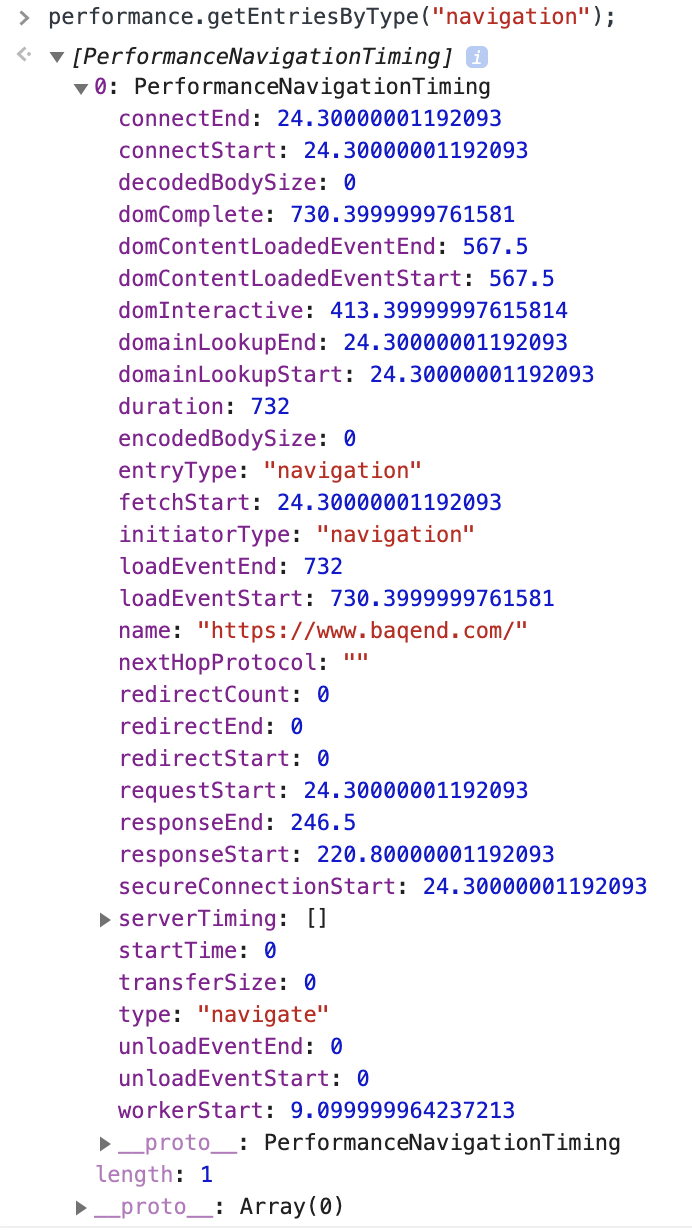
\includegraphics[width=0.4\textwidth]{navigation_console.png}
\caption{Navigation Timings}
\label{img:navigation_console}
\end{center}
\end{figure}


%TODO add this ?

% 2013 Grigorik
%- The real benefit of Navigation Timing is that it exposes a lot of previously inaccessible data, such as DNS and TCP connect times, with high precision (microsecond timestamps), via a standardized performance.timing object in each browser.
%- Hence, the data gathering process is very simple: load the page, grab the timing object from the user’s browser, and beacon it back to your analytics servers!
%- By capturing this data, we can observe real-world performance of our applications as seen by real users, on real hardware, and across a wide variety of different networks.

% 2013 Meenan
%- The largest benefit of navigation timing is that it exposes a lot of timings that lead up to the HTML loading --> This is this famous image
%- In addition to providing a good start time, it exposes information about any redirects, DNS lookup times, time to connect to the server, and how long it takes the Web server to respond to the request, for every user and for every page the user visits
%- The measurement points are exposed to the DOM (Document Object Model) through the performance object and make it trivial to calculate load times (or arbitrary intervals, really) from JavaScript.

% https://developer.mozilla.org/en-US/docs/Web/API/PerformanceNavigationTiming
%PerformanceNavigationTiming Interface: 
%- extends PerformanceEntry Interface from performance timeline. see attributes section for details
%- extends PerformanceResourceTiming Interface from resource timing


% ---------------------------------------------



\paragraph{Resource Timing}


% [Introduction]

Two versions of Resource Timing exist.
A Candidate Recommendation, Resource Timing Level 1, from March 2017, % https://www.w3.org/TR/resource-timing-1/
and Resource Timing Level 2, a Working Draft from April 2021.  % https://www.w3.org/TR/resource-timing-2/

As described above, while Navigation Timing exposes timing information for the main document, Resource Timing exposes timing information for all other resources the main document requests, and also resources other resources request.
Other resources may be CSS, JS, other HTML documents, images, and so on.
% https://www.w3.org/TR/resource-timing-2/

The exposed time stamps from Resource Timing are mainly network related timing values (see table X.)
For example, the time it takes to download a specific resource.


% [PerformanceResourceTiming Interface]

The values are exposed by the PerformanceResourceTiming interface and can be retrieved via $window.performance.getEntriesByType("resource")$.

% https://w3c.github.io/perf-timing-primer/
%- The PerformanceResourceTiming interface extends the PerformanceEntry interface in the Performance Timeline
%- Each of these timestamps is in microseconds, which are provided by the window.performance.now() method in the High Resolution Time specification.


% [Navigation and Resource Timing]

% https://www.w3.org/TR/resource-timing-2/
%- Navigation Timing 2 extends this specification to provide additional timing information associated with a navigation.
%- mechanisms to provide complete client-side latency measurements within applications

Navigation and Resource Timing go hand in hand.
With Navigation and Resource Timing, all relevant timing information for all resources of the website are available.
The Waterfall Chart (see section X.) is a picturesque example of a visualization of the exposed attributes by both specifications.

Figure X. depicts the values exposed by Navigation and Resource Timing.
Those attributes will be discussed next.




% ---------------------------------------------



\paragraph{Navigation and Resource Timing Attributes}

All timing values, or attributes, relevant for the navigation process and exposed by Navigation and Resource Timing Level 2, are listed in table X and figure X.
The black coloured time stamps assigned to the blue boxes in figure X. are captured by Navigation Timing.
The yellow time stamps are exposed by Resource Timing.
All attributes are retrievable via $performance.getEntriesByType("navigation")$.\footnote{They are exposed to navigation due to interface inheritance. For more details cf. } %cite navigation timing 2 spec
Figure X. does not include all defined and available values from the specification definitions, but only those important within the navigation process.
For documents from different origins, the attributes in parenthesis may not be available.% cite https://www.w3.org/TR/navigation-timing-2/#processing-model

\begin{figure}[h!]
\begin{center}
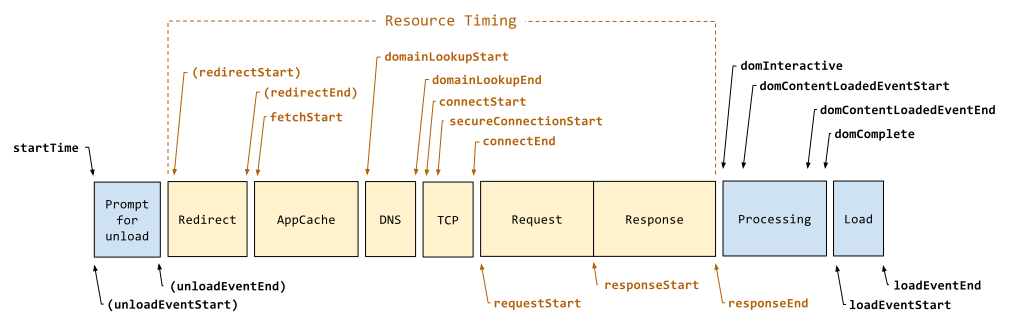
\includegraphics[width=1\textwidth]{timestamp_diagram.png}
\caption{Timestamps from Navigation and Resource Timing}
\label{img:latency}
\end{center}
\end{figure}
% cite https://www.w3.org/TR/navigation-timing-2/


Table X gives a short explanation for each time stamp.
The definitions are taken directly from the W3C specifications or MDN Web Docs, if not stated otherwise.
These time stamps are used to calculate performance metrics, as described in the next section.


%TODO is it ok to copy paste here from specs and MDN ?

\begin{center}
	\small
	\begin{longtable}{ | p{0.3\linewidth} | p{0.6\linewidth} | }
	\hline
	\multicolumn{2}{|c|}{ \cellcolor{lightgrey} Navigation Timings Level 2} \\
	\hline
	startTime (= navigationStart) & Start time of the navigation process. Is set to 0.  Navigation Timeline Level 1 exposes "navigationStart" which is set to the "time immediately after the user agent finishes prompting to unload the previous document."\footnote{\url{https://www.w3.org/TR/navigation-timing/)} [15.07.2021]} As some metric calculations still rely on navigationStart as seen below, it is mentioned here. \\
	\hline
	unloadEventStart & Set to 0 if there is no previous document. Otherwise, value is set to time when previous documents unload event gets fired by the user agent. \\
	\hline
	unloadEventEnd & Set to 0 if there is no previous document.  .Otherwise, value is set to time when previous documents unload event ends. \\
	\hline
	domInteractive & Time value equal to the time immediately before the user agent sets the current document readiness of the current document to "interactive". \\
	\hline
	domContentLoadedEventStart & Time value equal to the time immediately before the user agent fires the DOMContentLoaded event at the current document. \\
	\hline
	domContentLoadedEventEnd & Time value equal to the time immediately after the current document's DOMContentLoaded event completes.  \\
	\hline
	domComplete & Time value equal to the time immediately before the user agent sets the current document readiness of the current document to "complete". \\
	\hline
	loadEventStart & Time value equal to the time immediately before the load event (window.onload ??) of the current document is fired.  Returns 0 if event has not been fired.  \\
	\hline
	loadEventEnd & Time value equal to the time when the load event of the current document is completed.  Returns 0 if event has not been fired or is not completed. \\

	\hline
	\multicolumn{2}{|c|}{ \cellcolor{lightgrey} Resource Timings Level 2} \\
	\hline
	redirectStart & Start time of the fetch which initiates the redirect. \\
	\hline
	redirectEnd & Marks timestamp which occurs immediately after receiving the last byte of the response of the last redirect. \\
	\hline
	fetchStart & Marks when the browser starts to fetch a resource. Does not mark when the browser makes a network request for a resource, but rather when it begins checking caches to see if a network request is even necessary.  \\ % cite https://developers.google.com/web/fundamentals/performance/navigation-and-resource-timing
	% Represents a timestamp immediately before the browser starts to fetch the resource. \\
	\hline
	domainLookupStart & Returns the timestamp immediately before the browser starts the domain name lookup for the resource. \\
	\hline
	domainLookupEnd & Returns the timestamp immediately after the browser finishes the domain name lookup for the resource. \\
	\hline
	connectStart & Returns the timestamp immediately before the user agent starts establishing the connection to the server to retrieve the resource. \\
	\hline
	secureConnectionStart & Returns a timestamp immediately before the browser starts the handshake process to secure the current connection.  \\
	\hline
	connectEnd & Returns the timestamp immediately after the browser finishes establishing the connection to the server to retrieve the resource.  \\
	\hline
	requestStart & When the browser issues the network request.  \\% cite https://developers.google.com/web/fundamentals/performance/navigation-and-resource-timing
	% Returns a timestamp of the time immediately before the browser starts requesting the resource from the server, cache, or local resource. \\
	\hline
	responseStart & Returns a timestamp immediately after the browser receives the first byte of the response from the server, cache, or local resource. \\
	\hline
	responseEnd & Returns a timestamp immediately after the browser receives the last byte of the resource or immediately before the transport connection is closed, whichever comes first. \\
	\hline
	\caption{Navigation and Resource Timing Level 2 Attributes} % needs to go inside longtable environment
	\label{tab:navigationtiming}
	\end{longtable}
\end{center}

%TODO check: is loadEventStart coming from window.onload or document.onload ?

%TODO add values from other interfaces such as duration ?
%from PerformanceEntry Interface:
%name
%entryType
%startTime
%duration

%TODO add exposed as DOMHighResTimeStamp ?


The document states and events mentioned above, such as DOMContentLoaded, and when they are fired by the user agent, are defined in the HTML standard.


%TODO add this when there is time...

% [Implementation Example Chrome]

% lets see how chromium is capturing domContentLoaded


% more infos here (probably level 1)
% https://community.akamai.com/customers/s/article/Using-Navigation-Timing-APIs-to-understand-your-webpage?language=en_US

% https://developers.google.com/web/fundamentals/performance/navigation-and-resource-timing
% Requests and responses:
%- fetchStart marks when the browser starts to fetch a resource. This is distinct from a request in that it doesn't mark when the browser makes a network request for a resource, but rather when it begins checking caches (e.g., HTTP and service worker caches) to see if a network request is even necessary.
%- workerStart marks when a request is being fetched from a service worker within a fetch event handler (if applicable). This will be always be 0 if a service worker isn't installed for the current page.



% ---------------------------------


\paragraph{Metrics calculated with Navigation and Resource Timing}

The attributes exposed by Navigation and Resource Timing are used to calculate common navigation timing metrics.
Table X. lists a selection of navigation timing metrics and how they are derived from the exposed attributes by Navigation and Resource Timing.
Figure X. provides a graphical overview of the metrics and which intervals they are reflecting.

As with business metrics (section X.), there is not one source of truth or a set of definitions for navigation timing metrics.
Still, when going through literature, a common set of navigation timings can be identified.
Literature sources are for example MDN Glossary %https://developer.mozilla.org/en-US/docs/Glossary
Google developers guides % https://developers.google.com/web/fundamentals/performance/navigation-and-resource-timing
Other performance specialists blog posts % cite https://gtmetrix.com/blog/browser-timings/
Research papers % cite % 2013 Wang % 2018 Netravali % 2019 Enghardt
Or documentation of common RUM tools % cite https://github.com/akamai/boomerang/blob/master/doc/methodology.md

The sources mentioned above explain the idea of the metrics sometimes rather in an informal way.
How exactly the metrics are implemented and calculated, e.g. which Navigation Timing attributes are used, is not all time the clear and is the responsibility of the RUM tools vendors and can only be checked directly in the source code.
It is therefore possible. due to the lack of metrics standardization and definition, that for the same metric, different calculations are being used.


%TODO add this ?

%- navigationStart is not in level 2
%- navigationStart is the same as startTime in level 2
%- Difference is that navigationStart is a EPOCH time stamp. The timings have to be calculated as differences to this timestamp
%- navigationStart just starts with 0, which makes all the other timestamps easier to read
%- many still use level 1 and navigationStart


%TODO sort those metrics according to their occurance

\begin{center}
	\small
	\begin{longtable}{ | p{0.3\linewidth} | p{0.6\linewidth} | }
	\hline
	Time to First Byte (TTFB)
	& $[responseStart - navigationStart]$ \\
	& Indicates when the user agent received the first byte of the websites data. \\
	& "Time it takes between the start of the request and the start of the response".  \\% cite https://developer.mozilla.org/en-US/docs/Glossary/time_to_first_byte
	%TODO add more here ?
	
	\hline
	Page Load Time (PLT)
	& $[loadEventStart - navigationStart]$ \\
	& The MDN Docs define PLT as the "time it takes for a page to load" and it is calculated as stated above.  \\ % cite https://developer.mozilla.org/en-US/docs/Glossary/Page_load_time	
	& Across multiple authors, PLT is defined as the time from navigation start until the load event\footnote{\url{https://developer.mozilla.org/en-US/docs/Web/API/Window/load_event} [16.07.2021]} has been fired.
	The load event is fired when the main document and its linked resources have been loaded. \\
	& Grigorik states that PLT "has been the de facto metric of the web performance world", but is nowadays inaccurate due to the shift from static websites to dynamic web applications which load resources differently (cf also 2018 Netravali) and \\ % https://www.stevesouders.com/blog/2013/05/13/moving-beyond-window-onload/
			
		%TODO more here ?
		% Akamai defines PLT similarly as the elapsed time from navigation start until the "page is completely available for the user to interact with", using also loadEventStart as the point when loading has finished.
		% cite https://github.com/akamai/boomerang/blob/master/doc/methodology.md, https://community.akamai.com/customers/s/article/Using-Navigation-Timing-APIs-to-understand-your-webpage?language=en_US
		%Wang et al define PLT as the "time between when the page is requested and when the DOMLoad event is fired", where the DOMLoad event is the load event.\footnote{\url{https://developer.mozilla.org/en-US/docs/Web/API/Window/load_event} [16.07.2021]}      % cite 2013 Wang
		% 2019 Enghardt
	
	\hline
	DNS Lookup Time
	& $[domainLookupEnd - domainLookupStart]$ \\
	& Time it takes for a DNS lookup.  \\
		% cite % https://developer.mozilla.org/en-US/docs/Web/Performance/Navigation_and_resource_timings#dns_lookup_time
		% cite https://developers.google.com/web/fundamentals/performance/navigation-and-resource-timing
	
	\hline
	TCP Handshake % / Server Connect Time ?
	& $[connectEnd - connectStart]$ \\
	& "The time it takes for the TCP handshake." \\ % cite https://developer.mozilla.org/en-US/docs/Web/Performance/Navigation_and_resource_timings#tcp
% https://community.akamai.com/customers/s/article/Using-Navigation-Timing-APIs-to-understand-your-webpage?language=en_US
% https://developer.mozilla.org/en-US/docs/Web/Performance/Understanding_latency
	% Also called Connection Time.  % https://developers.google.com/web/fundamentals/performance/navigation-and-resource-timing

	\hline
	TLS Handshake Time
	& Time it takes to secure connection with TLS.  \\
	& MDN Docs defines TLS time with $[requestStart - secureConnectionStart]$ \\
	& Google defines TLS Time as $[connectEnd - secureConnectionStart]$ \\ % https://developers.google.com/web/fundamentals/performance/navigation-and-resource-timing

	\hline
	Request Time, 
	& $[responseStart - requestStart]$ \\ 
	Server Response Time & How long it takes for the request. \\ % cite https://developer.mozilla.org/en-US/docs/Web/Performance/Navigation_and_resource_timings#request_time
	& Also called Server Response Time by Akamai \\ % https://community.akamai.com/customers/s/article/Using-Navigation-Timing-APIs-to-understand-your-webpage?language=en_US
	
	\hline
	DOM Content Loaded,DOM Content Load
	& MDN defines DOM Content Loaded as $domContentLoadedEventEnd - domContentLoadedEventStart$, that is the DOMContentLoaded event duration. \\
		% https://developer.mozilla.org/en-US/docs/Web/Performance/Navigation_and_resource_timings#domcontentloaded_event
		% https://developer.mozilla.org/en-US/docs/Web/API/Window/DOMContentLoaded_event
	& Akamai defines a "DOM Content Load" time which represents the time from navigation start until the DOMContentLoaded event has been fired, captured by domContentLoadedEventEnd. \\
		% https://community.akamai.com/customers/s/article/Using-Navigation-Timing-APIs-to-understand-your-webpage?language=en_US		

	\hline
	Page Download Time,
	& $[responseEnd - responseStart]$ \\
	Receiving Time,  & How long it takes to download the page. \\
	Transfer Time & Also called Transfer time by Akamai or Receiving Time by MDN \\
	% https://community.akamai.com/customers/s/article/Using-Navigation-Timing-APIs-to-understand-your-webpage?language=en_US
	% https://developer.mozilla.org/en-US/docs/Web/Performance/Understanding_latency

	\hline
	Latency
	& $[responseStart - fetchStart]$ \\ 
	& Latency is defined as the elapsed time from when the browser requests the resource until the first byte from it is received.  \\ % cite https://community.akamai.com/customers/s/article/Using-Navigation-Timing-APIs-to-understand-your-webpage?language=en_US
		% cite https://developer.mozilla.org/en-US/docs/Web/Performance/Understanding_latency

	\hline
	DOM Interactive
	& $[domInteractive - navigationStart]$ \\
	& When the "browser has completed parsing the entire HTML and constructed the DOM" \\ % https://community.akamai.com/customers/s/article/Using-Navigation-Timing-APIs-to-understand-your-webpage?language=en_US

	
%TODO add this? maybe check again after WPT done
%	\hline
%	DOM Complete &
%	\begin{itemize}[label={}, noitemsep,nolistsep, leftmargin=0cm]
%		\item 
%		\item 
%	\end{itemize} \\	

%	\hline
%	Redirect &
%	\begin{itemize}[label={}, noitemsep,nolistsep, leftmargin=0cm]
%		\item 
% https://developers.google.com/web/fundamentals/performance/navigation-and-resource-timing
% redirectStart and redirectEnd 
%	\end{itemize} \\

	\hline
	\caption{Metrics} % needs to go inside longtable environment
	\label{tab:navigationtiming_metrics}
	\end{longtable}
\end{center}


%TODO add this to PLT ? as it is the same...
% window.onload:

% https://community.akamai.com/customers/s/article/Using-Navigation-Timing-APIs-to-understand-your-webpage?language=en_US
% Onload = loadEventEnd - loadEventStart -> not the same as PLT

% https://www.stevesouders.com/blog/2013/05/13/moving-beyond-window-onload/
% when window.onload() is fired

% https://speedcurve.com/blog/rendering-metrics/
% when window.onload() is fired



%TODO add this ?

% DOM Processing to Interactive
% https://community.akamai.com/customers/s/article/Using-Navigation-Timing-APIs-to-understand-your-webpage?language=en_US

% DOM Interactive to Complete
% https://community.akamai.com/customers/s/article/Using-Navigation-Timing-APIs-to-understand-your-webpage?language=en_US

%Load Event Duration
% https://developer.mozilla.org/en-US/docs/Web/Performance/Navigation_and_resource_timings#load_event_duration
%load = timing.loadEventEnd - timing.loadEventStart 


% Duration
% https://developer.mozilla.org/en-US/docs/Web/Performance/Navigation_and_resource_timings#duration
% duration = PerformanceNavigationTiming.loadEventEnd - PerformanceEntry.startTime
% -> duration from performanceentry interface is from loadEventStart - start Time

% Loading
% https://developers.google.com/web/fundamentals/performance/navigation-and-resource-timing
%- loadEventStart and loadEventEnd

% Document processing
% https://developers.google.com/web/fundamentals/performance/navigation-and-resource-timing
%- domInteractive, domContentLoadedEventStart, domContentLoadedEventEnd, and domComplete

% Unloading
% https://developers.google.com/web/fundamentals/performance/navigation-and-resource-timing
%Document unloading:
%- unloadEventStart and unloadEventEnd 

% Sizes
% https://developers.google.com/web/fundamentals/performance/navigation-and-resource-timing
% Document and resource size:
%- transferSize is the total size of the resource including HTTP headers.
%- encodedBodySize is the compressed size of the resource excluding HTTP headers.
%- decodedBodySize is the decompressed size of the resource (again, excluding HTTP headers).



\begin{figure}[h!]
\begin{center}
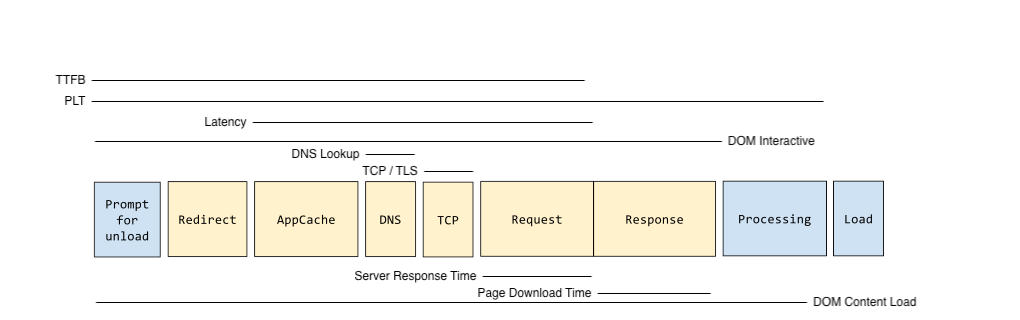
\includegraphics[width=1\textwidth]{nav_metrics.png}
\caption{Navigation Timing Metrics}
\label{img:latency}
\end{center}
\end{figure}
%TODO make this nicer, e.g. use same font as text for labels




% ------------------------------------------------
% ------------------------------------------------



Apart from Navigation and Resource Timing, the Web Performance Working Group also maintains other performance related specifications.
Some of them will be briefly discussed next.


\paragraph{User Timing}

User Timing Level 2 is a Recommendation from February 2019 and User Timing Level 3 is a Working Draft from July 2021.
User Timing provides methods to create own, specific and unique high resolution timestamps, to query them and to calculate intervals and the elapsed time between those created timestamps.% cite https://www.w3.org/TR/user-timing-3/
User Timing simplifies and facilitates the usage of custom metrics (see section X.)

% https://www.w3.org/TR/user-timing-3/
%- PerformanceMark and PerformanceMeasure interfaces

% Measuring Real User Performance in the Browser https://www.youtube.com/watch?v=yrWLi524YLM&ab_channel=NicJansma
%-> Puts data in Performance Timeline / DevTools


% -------------------


\paragraph{Performance Timeline}

Performance Timeline is a Recommendation from December 2013 % https://www.w3.org/TR/2013/REC-performance-timeline-20131212/
and Performance Timeline Level 2 is a Working Draft from June 2021. % https://www.w3.org/TR/performance-timeline-2/

In short, the Performance Timeline defines an API and methods which expose all timing values captured by other specifications such as Navigation or Resource Timing.
Performance Timeline defines an interface to acquire a variety of performance measurements. 
As already described, in can be used to retrieve Navigation Timings with $performance.getEntriesByType("navigation")$.

Additionally, a PerformanceObserver interface is defined, which can be used to monitor the Performance Timeline and notify as soon as new measurements and recordings are available.


%TODO add this ? is not so important...

% https://www.w3.org/TR/performance-timeline-2/
%- extends the High Resolution Time specification
%- providing methods to store and retrieve high resolution performance metric data.
%- Performance Timeline  defined by Navigation timing, resource timing, user timing and other interfaces
%- get Entries, by Type, by Name
%- Example entryType values defined by other specifications include: "mark" and "measure" [USER-TIMING-2], "navigation" [NAVIGATION-TIMING-2], "resource" [RESOURCE-TIMING-2], and "longtask"


% [Performance Entry]
	
% https://developer.mozilla.org/en-US/docs/Web/API/Performance_Timeline
%- PerformanceEntry interface encapsulates a single performance entry: a single data point or metric in the performance timeline


% https://developer.mozilla.org/en-US/docs/Web/API/PerformanceEntry
%- A performance entry can be directly created by making a performance mark or measure

%Always of type:
%- PerformanceMark
%- PerformanceMeasure
%- PerformanceFrameTiming
%- PerformanceNavigationTiming
%- PerformanceResourceTiming
%- PerformancePaintTiming

%Properties:
%- name
%- entryType
%- startTime
%- duration



% ----------------------------


\paragraph{Long Tasks}

Long Tasks API 1 has been released as a First Public Working Draft in September 2017.
The goal of the API is to detect "long tasks", this are tasks that occupy main thread for more than 50ms.
Long tasks are critical for performance as they block other critical tasks such as user input. % cite  https://www.w3.org/TR/longtasks-1/

%TODO
Long Tasks API is a basis to calculate metrics such as  Time to Interactive (TTI) and Total Blocking Time (TBT). % https://web.dev/custom-metrics/#long-tasks-api
TTI and TBT will be discussed below.

% https://github.com/WICG/time-to-interactive


% https://www.youtube.com/watch?v=6Ljq-Jn-EgU&ab_channel=GoogleChromeDevelopers
%- Long Tasks: Is it delightful? PerformanceObserver


% ----------------------------


\paragraph{Server Timing}

Server Timing is a Working Draft from June 2021.
With specifications such as Navigation and Resource Timing, the user agent has access to a variety of different timings regarding the navigation process.
Not visible nor available are measurement and timings within the server processing, e.g. database queries.
Server Timing addresses this problem by enabling a server to transfer and communicate performance related information to the user agent. % cite https://www.w3.org/TR/server-timing/



% ----------------------------


\paragraph{Paint Timing}

Paint Timing 1 has been released as a First Public Working Draft in September 2017.  
It specifies two "key moments" during the load process: First Paint (FP), and First Contentful Paint (FCP).
Table X. provides explanations for the key moments as they are defined in the specification. % cite https://www.w3.org/TR/paint-timing/

The metrics can be retrieved directly in the browser via $performance.getEntriesByType("paint")$.
Hence, FP and FCP can be collected in RUM.
Other visual metrics rely mostly on video analysis and need a synthetic monitoring setup, as described in the next section.

\begin{center}
\small
	\begin{tabular}{ | p{0.3\linewidth} | p{0.6\linewidth} | }
	\hline
	First Paint & Marks the point when the browser renders anything that is visually different from what was on the screen prior to navigation \\ 
	\hline
	First Contentful Paint & The point when the browser renders the first bit of content from the DOM, which may be text, an image, SVG, or even a canvas element \\  
	\hline
	\end{tabular}
\end{center}


FP and FCP indicate when the user sees something different than the default white screen for the first time.
If the visual change is important or useful for the user is not reflected by FP or FCP. % cite 2013 Meenan

%TODO
As described below, FCP is part of Google's Web Vitals.
For a more fine grained measurement, they enhance the default metric.



%TODO add more here ?

% https://developer.mozilla.org/en-US/docs/Glossary/First_paint
% https://developer.mozilla.org/en-US/docs/Glossary/First_contentful_paint

% A user centric metric pendant is Start Render.
% FP and FCP are visual metrics from a browsers perspective, and not from a users perspective, as they are derived from  and not the actual pixels on the screen.



% ----------------------------


%TODO write this down and add to summary table

\paragraph{Element Timing API and Event Timing API}

Unofficial drafts

% https://wicg.github.io/element-timing/

% https://wicg.github.io/event-timing/


% https://web.dev/custom-metrics/
Element TIming used for LCP
Event Timing used for FID




% ------------------------------------------------------------------------------------------------------------------



\subsubsection{Navigation Timing Metrics Conclusion}

[tbd]

We can measure time for different processes in the document loading process.
W3C and the Performance Working Group especially maintain and define a set of specifications with the task to measure performance related data.
The attributes exposed by there specifications are used to calculate performance or navigation timing metrics.

As the performance metrics are not officially defined by any authorizes party or institution, their meaning may diverge depending on the implementation.

Table X provides an overview of all discussed specifications, in which maturity level they are available and why they are important.


%The High Resolution Time recommendation enables exact, stable and reliable time measures.
%The Navigation and Resource Timing specifications expose all relevant time stamps on the document, or any resource respectively, loading process.
%The User Timing spec makes it possible for analysts and developers to mark and measure custom time stamps and expose them directly to the Performance Timeline.
%The Performance Timeline subsumes all exposed timing measures and is the go to place to fetch performance data.

%Or as Grigorik states it, "The combination of Navigation, Resource, and User timing APIs provides all the necessary tools to instrument and conduct real-user performance measurement for every web application" % cite 2013 Girgorik


\begin{center}
\small
	\begin{tabular}{ p{0.3\linewidth} | p{0.6\linewidth} }
	High Resolution Time
	& Level 2: REC November 2019 \\
	& WD July 2021 \\
	& Provides exact, stable and reliable time measures \\
	\hline
	Navigation Timing
	& Level 1: REC December 2021 \\
	& Level 2: WD March 2021 \\
	& Exposes navigation timing information of the main document \\
	\hline
	Resource Timing
	& Level 1: CR March 2017 \\
	& Level 2: WD April 2021 \\
	& Exposes timing information from requested resources and the resources they request.  \\
	\hline
	Navigation and Resource Timing
	& Used to calculated a variety of metrics \\
	\hline
	\hline
	User Timing
	& Level 2: REC February 2019 \\
	& Level 3: WD July 2021 \\
	& Mark and measure custom timestamps \\
	\hline
	Performance Timeline
	& REC December 2013 \\
	& Level 2: WD June 2021 \\
	& Subsumes gathered performance data from other specifications \\
	\hline
	Long Tasks
	& API 1: FPWD  September 2017 \\
	& Identifies tasks occupying main thread for more than 50ms \\
	& Basis for TTI and TBT \\
	\hline
	Server Timing
	& WD June 2021 \\
	& Standard to transmit performance related data from the server to the client \\
	\hline
	Paint Timing
	& FPWD September 2017 \\
	& Exposes the "key moments" First Paint and First Contentful Paint \\
	\end{tabular}
\end{center}


% [Transition]

Paint Timing already shoots in a direction which tries to measure user perceived performance not just by measuring elapsed time between navigation events, but rather observe visual changes during the websites loading process.
When navigation timings can help to identify eventual bottlenecks or other technical debts during the loading process, they do not reflect how the actual user is perceiving the performance of the websites loading process.
As users consume websites mainly with the eyes, visual indicators are relevant and of crucial importance.

A variety of visual and user-centric performance metrics emerged in the last years, with Google promoting some of them.
They will be discussed in the next section.



% -----------------------------------------------------------------------
% -----------------------------------------------------------------------



\subsection{User-Centric Performance Metrics}


[tbd]


% [Introduction]

Navigation Timings as described above are directly measured through a variety of Web APIs and are accessible within the browser.
Metrics concerned with user-perceived performance focus mainly on visual changes of the website and can thereby not be captured directly through Web APIs.

Perceived performance tackles the question how fast a website "feels" to a user.
As already described in section X. different users feel performance differently, depending on factors such as gender, region or stress level.
The perceived performance can diverge from actual loading times, and user-centric performance metrics are usually more difficult to measure than navigation timings, as visual or even video analysis is necessary to calculate the metrics. % cite https://developer.mozilla.org/en-US/docs/Learn/Performance/Perceived_performance

I will describe user-centric performance metrics which are established among performance monitoring solution vendors.
With Web Vitals, Google defines their own set of user-centric metrics and moves websites performance into focus.
They will be discussed below.



% ------------------------

\subsubsection{Visual Metrics}

[tbd]





% ------------------------



\paragraph{Start Render, Time to First Paint (TTFP)}

The Start Render time is the time when the browser rendered the first pixel on the screen visible for the user.
Start Render is calculated through video analysis instead of levering browser APIs such as Paint Timing.
% cite  https://blog.dareboost.com/en/2019/09/first-contentful-paint-fcp/

Start Render is defined and exposed by a variety of synthetic monitoring solutions such as speedcurve or WebPageTest.
% cite https://support.speedcurve.com/en/articles/74078-what-do-the-different-speedcurve-metrics-represent
% cite https://docs.webpagetest.org/metrics/page-metrics/

Netravali et al. use the term Time to First Paint (TTFP) for the very same metric, % cite 2018 Netravali
whereas for Enghardt et al. , TTFP is the same as FP, which is measured within the browser and not through video analysis. % 2019 Enghardt

This example reveals that the definitions of metrics is not clear and different authors use different definitions.





% ------------------------


\paragraph{Above the Fold Time (AFT)}

The above-the-fold is the area of the website which is visible to the user without scrolling.
The AFT metric measures how long it takes the browser to render all pixel within that above the fold area.
AFT measurement needs to take into consideration visual dynamic areas of the website which are expected to change pixels frequently and static areas where pixel and color changes are not likely to happen. % 2018 Netravali

AFT is measurable through synthetic monitoring and requires video recording and analysis. % cite 2013 Meenan

The AFT is not standardized. % 2019 Enghardt



% ------------------------


\paragraph{Speed Index (SI)}

The Speed Index (SI) is a metric invented by the founders of WebPageTest and aims to express user experience in a single number. % cite 2013 Meenan

Like the AFT, the SI reflects the visual completeness of the website.
Where as AFT only measures the single point in time when the viewport is fully rendered, SI also takes the visual loading progress of the website into consideration and reflects "the average time at which visible parts of the page are displayed". % % 2018 Netravali  https://docs.webpagetest.org/metrics/speedindex/
SI is not directly measured, but calculated, and expressed in milliseconds. % https://gtmetrix.com/speed-index.html

Like AFT, SI is reliable for static websites and unreliable for websites with dynamic and changing visual content. % https://medium.baqend.com/mobile-site-speed-measurement-best-practices-ff4a3f91b003
The SI calculation details are covered in % https://docs.webpagetest.org/metrics/speedindex/




% 2021 Meenan vimeo 38:50


% Measuring Real User Performance in the Browser
%- How much of the screen is visually available at different points of time
%- At what point of time is the page complete



% ------------------------


\subsubsection{Web Vitals}


% [Introduction]

With the Web Vitals initiative, Google joins the web performance metrics discussion.
Their goal is to "provide unified guidance for quality signals that are essential to delivering a great user experience on the web." % https://web.dev/vitals/
The unified guidance consists of the Web Vitals, a set of performance metrics, focussing on how the users experience and perceive performance, contrary to the mere navigation timings as discussed in section X.
With performance being a factor in Google search rankings, Web Vitals become automatically important for website operators. % https://developers.google.com/web/updates/2018/07/search-ads-speed

% [Evolving]

The set and definitions of Web Vitals metrics are not set in stone, but are constantly evolving.
The definitions, calculations, recommended thresholds, or even the metrics themselves may change over time, always adapted to the rapidly evolving technologies of the WWW and advances in web performance. % https://web.dev/vitals/
While Web Vitals are currently primarily about web performance, other aspects of usability, such as security, privacy, or accessibility, will be included in the future. % https://www.youtube.com/watch?v=iNfz9tg-wyg&ab_channel=GoogleChromeDevelopers

% [Definition and Key Questions]

Web Vitals and their definitions are derived from a set of key questions (table X.).
The key questions reflect what users may (eventually unconsciously) ask while consuming a website. 
This user-centric framework guides and sets the agenda for creating and defining Web Vitals metrics.
Contrary to navigation timing metrics, the Web Vitals focus are users and their perception, and each question is a perspective or facet of user experience.
Web Vitals are "metrics relevant to users". % https://web.dev/user-centric-performance-metrics/

 
\begin{center}
\small
	\begin{tabular}{  p{0.3\linewidth} | p{0.6\linewidth}  }
	\textit{Is it happening?} & Did the navigation start successfully? Has the server responded? \\
	\hline
	\textit{Is it useful?} & Has enough content rendered that users can engage with it? \\
	\hline
	\textit{Is it usable?} & Can users interact with the page, or is it busy? \\
	\hline
	\textit{Is it delightful?} & Are the interactions smooth and natural, free of lag and jank? \\
	\end{tabular}
\end{center}
 % cite https://web.dev/user-centric-performance-metrics/


% [Types of Metrics]

In addition to the key questions, Google identifies different aspects or types of a website's performance.
Like the key questions, these types provide a guide and framework to organize, classify, and integrate Web Vitals. % https://web.dev/user-centric-performance-metrics/

%TODO add more here, some interpretation ?

\begin{center}
\small
	\begin{tabular}{  p{0.3\linewidth} | p{0.6\linewidth}  }
	\textit{Perceived load speed} & How quickly a page can load and render all of its visual elements to the screen. \\
	\hline
	\textit{Load responsiveness} & How quickly a page can load and execute any required JavaScript code in order for components to respond quickly to user interaction. \\
	\hline
	\textit{Runtime responsiveness} & After page load, how quickly can the page respond to user interaction. \\
	\hline
	\textit{Visual stability} & Do elements on the page shift in ways that users don't expect and potentially interfere with their interactions? \\
	\hline
	\textit{Smoothness} & Do transitions and animations render at a consistent frame rate and flow fluidly from one state to the next? \\
	\end{tabular}
\end{center}
%cite  https://web.dev/user-centric-performance-metrics/


% [Measurement and Tools]

Web Vitals can be measured through synthetic monitoring or RUM. % https://web.dev/user-centric-performance-metrics/
For example, RUM data is available through CrUX\footnote{\url{https://developers.google.com/web/tools/chrome-user-experience-report} [22.07.2021]}, synthetic data is available through Lighthouse\footnote{\url{https://developers.google.com/web/tools/lighthouse} [22.07.2021]}.
A custom JS library is available an can be integrated into any website to capture Web Vitals.\footnote{\url{https://github.com/GoogleChrome/web-vitals} [22.07.2021]}

%PageSpeedInsigths ?



% [Outline]

In the following, I will describe common Web Vitals metrics.
Afterwards, Core Web Vitals,Web Vitals that matter the most, will be discussed.



% ------------------------


\paragraph{First Contentful Paint}

FCP tackles the question \textit{Is it happening?} and is classified as the type \textit{Perceived load speed}.
This is the same FCP as exposed by Paint Timing (see section X.), and "marks the first point in the page load timeline where the user can see anything on the screen". % https://web.dev/fcp/

Google enhances the Paint Timing specification regarding FCP by only considering pages that are in the foreground all the time,
by measuring FCP also if the page has been loaded from cache, and by exposing FCP for all frames, including cross-origin iframes.
Implementation details are available within the web-vitals library.\footnote{\url{https://github.com/GoogleChrome/web-vitals/blob/main/src/getFCP.ts} [22.07.2021]}

FCP is measured in seconds and available through synthetic or real-user monitoring.
% https://web.dev/fcp/






% ------------------------


\paragraph{First Meaningful Paint}

FMP is "the paint after which the biggest above-the-fold layout change has happened and web fonts have loaded". % https://developer.mozilla.org/en-US/docs/Glossary/first_meaningful_paint

Google states that FMP is deprecated, due to "inconsistent results" and the impossibility to measure it in all web browsers. % https://web.dev/first-meaningful-paint/
The successor, Largest Contentful Paint, is discussed below.
The replacement of FMP nicely illustrates the evolving nature of Web Vitals.


% https://medium.baqend.com/mobile-site-speed-measurement-best-practices-ff4a3f91b003
%The First Meaningful Paint is another user-centric metric and represents the point in time at which the largest visual change takes place; the underlying assumption here obviously is that the biggest visual change is relevant to the user, for example because a hero image or a navigation bar appear



% ------------------------


\paragraph{Time to Interactive, First CPU Idle}



%Not a Web Vitla ? % https://github.com/GoogleChrome/web-vitals#api

%in essence, TTI indicates when the browser or website is able to respond quickly to user input.
%Technical details diverge of how to measure TTI

%As with other metrics, a clear definition is not given and there are some variants and the metrics evolutes.

% https://github.com/WPO-Foundation/webpagetest/blob/master/docs/Metrics/TimeToInteractive.md
%- two variations exist:
%- Time to Consistently Interactive (WICG ) -> is normal TTI. Implementation different between WICG and Google
%- First CPU Idle (First Interactive)


% https://developer.mozilla.org/en-US/docs/Glossary/First_interactive
%First CPU Idle is the same as First Interactive
%MDN states that TTI exists in 2 variations: First Interactive, Consistently Interactive


% 2018 Netravali
%- "The standard’s definition of TTI is still in flux"
%- definitions uses a starting point, FCP or FMP, network requests and main thread idle




% [WICG]

% https://github.com/WICG/time-to-interactive
%- Defined by WICG, indicates when the website becomes interactive.


% https://developer.mozilla.org/en-US/docs/Glossary/Time_to_interactive
%"Time to Interactive (TTI) is a non-standardized web performance 'progress' metric defined as the point in time when the last Long Task finished and was followed by 5 seconds of network and main thread inactivity."


% [Google]

%web vital

% https://docs.google.com/document/d/1GGiI9-7KeY3TPqS3YT271upUVimo-XiL5mwWorDUD4c/edit
%Google has 2 metrics:
%- Fist CPU idle
%- Time to Interactive
% -> Fist CPU idle is deprecated again % https://web.dev/first-cpu-idle/



% https://web.dev/tti/
% - a little bit different definition by Google



% ------------------------


\paragraph{Total Blocking Time}

% https://web.dev/tbt/








% ----------------------------------------
% Core Web Vitals
% ----------------------------------------


\paragraph{Core Web Vitals}

Within the set of Web Vitals, there is a group of metrics that matter the most.
The Core Web Vitals are structured around the performance aspects loading, interactivity, and visual stability.
Each of three Core Web Vitals reflects one of those aspects (table X.).

The Core Web Vitals are relevant for all kinds of websites and can be measures or retrieved in all Google tools.

Contrary to the general evolving Web Vitals, Core Web Vitals are rather stable in terms of definitions, but also recommended benchmarks.

% https://web.dev/vitals/
%- each is measurable in the field

%- Collected by Crux, Pagespeed insights and search console



%- measure with library % https://github.com/GoogleChrome/web-vitals

\begin{center}
\small
	\begin{tabular}{  p{0.3\linewidth} | p{0.6\linewidth}  }
	\textit{Largest Contentful Paint (LCP)} & Measures loading performance.  \\
	\hline
	\textit{First Input Delay (FID)} & Measures interactivity. \\
	\hline
	\textit{Cumulative Layout Shift (CLS)} & Measures visual stability.  \\
	\end{tabular}
\end{center}

The three Core Web Vitals will be discussed in more detail below.



% --------------------



\paragraph{Core Web Vital: Largest Contentful Paint}



% LCP https://web.dev/lcp/


% https://www.youtube.com/watch?v=iNfz9tg-wyg&ab_channel=GoogleChromeDevelopers
%- LCP: Progressive loading.
%- FCP may become a core web vital



% https://wicg.github.io/largest-contentful-paint/



% https://medium.baqend.com/mobile-site-speed-measurement-best-practices-ff4a3f91b003
%- approximation of the First Meaningful Paint that can be captured in the browser




% [Measuring]
 
%- Google had some issues with capturing LCP in chrome, see twitter
%- Because of this they needed to release a new chrome version
%- CruX also has 2 different lcps now (?)
%- use this story to show that this stuff is far from trivial



% --------------------------


\paragraph{Core Web Vital: First Input Delay}

% FID https://web.dev/fid/


% https://www.youtube.com/watch?v=iNfz9tg-wyg&ab_channel=GoogleChromeDevelopers
%- FID: Interactivity during load


% [Measuring]



% --------------------------


\paragraph{Core Web Vital: Cumulative Layout Shift}

% CLS https://web.dev/cls/


% https://www.youtube.com/watch?v=iNfz9tg-wyg&ab_channel=GoogleChromeDevelopers
%- CLS: Visual stability


% [Measuring]


% New Measurement https://blog.webpagetest.org/posts/understanding-the-new-cumulative-layout-shift/?utm_medium=email&_hsmi=121601471&_hsenc=p2ANqtz-9IsSdXActEE6lw4BrDZNa4eFqzQZjgabLHbq7aS-c2KkhqLGNtkIaGfQYD4VqZe9_6ZYFlTmlCgB87THSfsnVM1fl7NiixtrJqAsVO6DPUjeJIo6c&utm_content=121601471&utm_source=hs_email


% --------------------------


\paragraph{Excursion: Thresholds and Benchmarks for Core Web Vitals}


[tbd]

% https://blog.chromium.org/2020/05/the-science-behind-web-vitals.html



% https://web.dev/defining-core-web-vitals-thresholds/



% [LCP]







% [FID]






% [CLS]









%TODO add this?
%- User perceived PLT



% -----------------------------------------------------------------------

% Conclusion


% Questions:

% Is it happening?
% FCP

% Is it useful?

% Is it usable?

% Is it delightful?




% Types:

% Perceived load speed
% FCP

% Load responsiveness

% Runtime responsiveness

% Visual stability

% Smoothness




% -----------------------------------------------------------------------
% -----------------------------------------------------------------------



\subsection{Custom Metrics}


[tbd]

% 2013 Meenan
%- First, it is important to understand that no single number will answer that question. Even if you have defined exactly what you are trying to measure on your Web site, performance will vary widely across your user base and across the different pages on your site
%- Nothing beats application-specific knowledge and measurements

% 2021 Meenan
%- own / user specific metrics, e.g. time to first tweet for twitter 


% 2013 Grigork
%- "there is no one single metric that holds true for every application, which means that we must carefully define custom metrics in each case"
%-  "Custom and application-specific metrics are the key to establishing a sound performance strategy"


% https://web.dev/custom-metrics/
%- Universal metrics offer a good baseline, but in many cases you need to measure more than just these metrics in order to capture the full experience for your particular site.
%- Custom metrics allow you to measure aspects of your site's experience that may only apply to your site


% https://web.dev/user-centric-performance-metrics/



% https://speedcurve.com/blog/user-timing-and-custom-metrics/



% -----------------------------------------------------------------------

\subsection{WebPageTest and Google Analytics Metrics}

[tbd]




% ----------------------------------------------------------------


\subsubsection{WebPageTest Metrics}

[tbd]

% https://docs.webpagetest.org/getting-started/


% [Metrics Categories according to WPT Docs]

% Metrics Categories:

	%  High Level Metrics:
		%  Document Complete
		%  Fully Loaded
		%  Load Time
		%  First Byte
		%  Start Render
		%  Requests
		%  Bytes In (Page Size)

	%  Page-level Metrics:

		%  Technical Page Metrics:
			%  -> APIs, GA Site Speed Metrics
			%  TTFB
			%  loadTime
			%  docTime
			%  ...

		%  Visual Metrics:
			%  SpeedIndex
			%  firstPaint
			%  firstContentfulPaint
			%  firstMeaningfulPaint
			%  ...

		%  Javascript and CPU timings
		%  Page Information
		%  Browser State
		%  Lighthouse Summary Metrics
		%  Optimization Checks/Grades
		%  Instrumented Metrics
		%  Test Information
		%  Misc

	%  Request-level metrics:
		%  Request Details
		%  Request Timings
		%  Request Stats
		%  Headers
		%  Protocol Information
		%  Javascript/CPU details
		%  Optimization Checks
		%  Misc	



	
%  [Optimization Grades]
	%  Keep-alive Enabled
	%  Compress Text
	%  Compress Images
	%  Cache Static Content
	%  Use of CDN


% [First View and Repeat View]



% Taken from WPT book p. 34, ...
% https://www.webpagetest.org/forums/showthread.php?tid=10315
% https://www.webpagetest.org/forums/showthread.php?tid=13266
% https://www.webpagetest.org/forums/showthread.php?tid=332
% https://www.webpagetest.org/forums/showthread.php?tid=10732
% https://www.webpagetest.org/forums/showthread.php?tid=12846



% Move those definitions to chapter above?
% Here i could only describe which metrics are available in WPT

\begin{center}
	\small
	\begin{longtable}{ p{0.3\linewidth} | p{0.6\linewidth} }
	Name & Description \\ 
	\hline
	Successful Tests & Amount of tests who completed successfully  \\
	
	Document Complete & ...  \\ % The time from the initial request until the browser fires load event. Also known as the document complete time. This is the time at which the Document Object Model (DOM) has been created and all images have been downloaded and displayed. For most traditional web pages, the load time is a suitable metric for representing how long a user must wait until the page becomes usable. This is the default performance metric on WebPageTest. Also known as Load Time (?). Around this time, the page's script is hard at work in the load-event handler firing off more requests for secondary content. The incomplete nature of this metric is why Fully Loaded was added to the table of metrics from the previous section. window.onload (?). The point where the browser onLoad event fires. The equivalent Navigation Timing event is loadEventStart. Document Complete Time: Amount of time that has elapsed from the initial page request until the browser fires the load event. This is the time at which the Document Object Model (DOM) has been created and all images have been downloaded and displayed. \\
	
	Fully Loaded & ...  \\ % The time from the initial request until WebPageTest determines that the page has finished loading content. The page might have waited for the load event to defer loading secondary content. The time it takes to load the secondary content is accounted for in the Fully Loaded Time. The time (in ms) the page took to be fully loaded — e.g., 2 seconds of no network activity after Document Complete. This will usually include any activity that is triggered by javascript after the main page loads. The point after onLoad where network activity has stopped for 2 seconds. Specific to WebPageTest and not provided by Performance API. Fully loaded waits for 2 seconds of no network activity (and no outstanding requests) after onLoad and then calls it done (only measures to the last activity, doesn't include the 2 seconds of silence in the measurement). Fully Loaded is a measure based on the network activity and is the point after onload when there was no activity for 2 seconds. \\
	
	First Byte & ...  \\ % Time until the server responds with the first byte of the response.  \\
	
	Start Render & ...  \\ % Time until the browser paints content to the screen. The time for the browser to display the first pixel of content (paint) on the screen. Time until the browser paints content to the screen. WebPageTest's own metric, determined by programmatically watching for visual changes to the page. Same as First Render? \\
	
	Bytes In (Doc) & ...  \\ % Total size of the Document Complete Requests' response bodies in bytes.  \\
	
	Requests (Doc) & ...  \\ % Number of HTTP requests before the load event, not including the initial request. \\
	
	Load Event Start & ...  \\ % Time in ms since navigation started until window.onload event was triggered (from W3C Navigation Timing). \\
	
	Speed Index	& ...  \\ % See Speed Index  \\
	
	Last Visual Change & ...  \\ % Time in ms until the last visual changed occured. Last change is a completely visual measurement and is the last point in the test when something visually changed on the screen. It could be something as simple as an animated gif or ad even that didn't really cause much CPU work but changed some pixels on the screen. It is only captured when video is recorded because it depends on the video capture to measure it. \\
	
	Visually Complete & ...  \\ % Time in ms when page was visually completed. Is measured from a video capture of the viewport loading and is the point when the visible part of the page first reached 100\% "completeness" compared to the end state of the test. \\
	\caption{Your caption here} % needs to go inside longtable environment
	\label{tab:myfirstlongtable}
	\end{longtable}
\end{center}




% https://speedcurve.com/blog/rendering-metrics/





% ----------------------------------------------------------------



\subsubsection{GA Site Speed Metrics}

[tbd]


% Default performance metrics captured by analytics.js.
% Show with analytics.js that it is indeed those navigation timing api calculations.
% Ec = function (a)...

% 2013 Girgorik: "Google Analytics automatically gathers Navigation Timing data when the analytics tracker is installed." ch. primer on web performance

% GA does not really provide any UX metrics! The site speed metrics are all from navigation timing api which are measurements from the browser.
% GA Site Speed Metrics (description from \url{https://support.google.com/analytics/answer/2383341?hl=en&ref_topic=1282106})
% \url{https://stackoverflow.com/questions/18972615/how-do-the-metrics-of-google-analytics-site-speed-map-to-the-w3c-navigation-timi}



\begin{center}
\small

	\begin{tabular}{ p{0.3\linewidth} | p{0.6\linewidth} }
	Name & Description  \\ 
	\hline
	Page Load Sample & The number of pageviews that were sampled to calculate the average page-load time.  \\
	
	Speed Metrics Sample & The sample set (or count) of pageviews used to calculate the averages of site speed metrics. This metric is used in all site speed average calculations, including avgDomainLookupTime, avgPageDownloadTime, avgRedirectionTime, avgServerConnectionTime, and avgServerResponseTime.  \\
	
	DOM Latency Metrics Sample & Sample set (or count) of pageviews used to calculate the averages for site speed DOM metrics. This metric is used to calculate ga:avgDomContentLoadedTime and ga:avgDomInteractiveTime.  \\

	Page Load Time (sec) & The average amount of time (in seconds) it takes that page to load, from initiation of the pageview (e.g., click on a page link) to load completion in the browser.  \\
	
	Domain Lookup Time (sec) & The average amount of time spent in DNS lookup for the page.  \\
	
	Page Download Time (sec) & The time to download your page.  \\
	
	Redirection Time (sec) & The time spent in redirection before fetching the page. If there are no redirects, the value for this metric is expected to be 0.  \\
	
	Server Connection Time (sec) & The time needed for the user to connect to your server.  \\

	Server Response Time (sec) & The time for your server to respond to a user request, including the network time from the user's location to your server.  \\
	
	Document Interactive Time (sec) & The average time (in seconds) that the browser takes to parse the document (DOMInteractive), including the network time from the user's location to your server. At this time, the user can interact with the Document Object Model even though it is not fully loaded.  \\

	Document Content Loaded Time (sec) & The average time (in seconds) that the browser takes to parse the document and execute deferred and parser-inserted scripts (DOMContentLoaded), including the network time from the user's location to your server. Parsing of the document is finished, the Document Object Model is ready, but referenced style sheets, images, and subframes may not be finished loading. This event is often the starting point for javascript framework execution, e.g., JQuery's onready() callback, etc.  \\
	\end{tabular}
\end{center}



% DNS Resolution = GAs Avg. Domain Lookup Time (sec) % https://metriclabs.com.au/glossary/analytics-metrics/avg-domain-lookup-time-sec/





% ----------------------------------------------------------------



\subsubsection{Comparison GA and WPT Metrics}

[tbd]

% We can show that above relations are true with experiments
% Load test page on a specific day only once and save timings exposed by performance.timing object (from console)
% Calculate differences corresponding to the table
% Get GA data for that day and save it


%TODO use graphical comparison ?


\begin{sidewaysfigure}

\begin{center}
	\begin{tabular}{ l | l | l }
	Navigation Timing API & WPT & GA \\ 
	\hline
	loadEventStart - navigationStart & Document Complete, Load Event Start & pageLoadTime \\
	domainLookupEnd - domainLookupStart & DNS lookup, dns\textunderscore ms & domainLookupTime \\
	connectEnd - connectStart & connect\textunderscore ms & serverConnectionTime \\
	responseStart - requestStart & .. & serverResponseTime \\
	responseEnd - responseStart & .. & pageDownloadTime \\
	fetchStart - navigationStart & .. & redirectionTime \\
	domInteractive - navigationStart & .. & domInteractiveTime \\
	domContentLoadedEventStart - navigationStart & domContentLoadedEventStart & domContentLoadedTime \\
	\end{tabular}
\end{center}


\end{sidewaysfigure}
















% -----------------------------------------------------------------------


\subsection{Web Performance Metrics Conclusion}


[tbd]

%TODO ideally come up with a nice table which abstracts and summarizes everything about metrics:
% e.g. measured by: browser, server. Technical stuff is measured in browser, everything else not in browser
% technical, UX, ...

[summary table]

% Navigation Timings: Coming from CRP, Loading Process, exposed by APIs
% User Centric: General visual metrics
% Web Vitals: Coming from key questions and types, measured with..., calculated by


[Link to Research Question]


\paragraph{Observer Effect}

[tbd]

% https://www.youtube.com/watch?v=yrWLi524YLM&ab_channel=NicJansma
%Avoiding the Observer Effect

%- How to measure performance without affecting performance?
%- JS is single threaded
%- Unless browser is idle, anything you do in JS will slow down some other JS
%-> Do only cheap stuff
%- Don't slow down load time:
%	- Load measurement code outside the critical path
%	- Use Iframe Loader Technique
%	- Load measurement code after onload event (-> can not measure things that happen before onload)

%- Do as little as possible in event handlers
%- Do more expensive processing via requestIdleCallback that runs when browser is idle



% https://web.dev/custom-metrics/
%The first rule of effective performance measurement is to make sure your performance measurement techniques aren't causing performance issues themselves.



%Before tackling this question with an experiment, I will discuss one synthetic monitoring tool WPT and one RUM tool GA which I will then use in the approach.
%Also some research in this field will be discussed.






\chapter{Related Research}
\label{chapter:related_work}


%TODO do again some research about optimizatzion / how to improve performance

% [Last chapter]

% [Research Question]

% no research that covers the same questions, e.g. how tracking scripts influence the performance of the website they measure
% a lot in this area is about optimization

% [This chapter: Why its here. Describe shortly all sections from this chapter]

% general research
% research about metrics
% research about tools

% [Next chapter]


% ----------------------------------------------------------------------


\section{General Research in the Field of Web Performance}

% 2011 Butkiewicz: Correlation between website complexity and its performance:
% -> Therefore it makes sense for me to use http archive inspired website approach, since page weight / page complexity impacts performance
% - Measures impact of website complexity on performance
% - Finds out that top 5 metrics that determine performance are:
% total number of objects loaded,  the number of these objects that are Javascripts,  the total web- page size,  and the number of servers and origins contacted in loading objects on the page.


% 2014 Singal: WEB ANALYTICS: STATE-OF-ART & LITERATURE ASSESSMENT
%\paragraph{2014 Singal}

%I.
%- Describes history of web analytics and tools
%- Provides definitions and taxonomy for metrics
%- Describes log file vs page tagging
%- Describes KPIs

%II.
%- Lit. overview for KPIs and Web Metrics
%- Lit. overview for "Trust"
%- Lit. overview for "Fuzzy"
%-> What are does categories?


%III.
%- Some other literature worth mentioning


%IV.
%- Describes 8 open challenges for researchers


%\paragraph{2015 Bekavac}

%- Two parts:
%	- 1: Some general overview of web analytics, tools and metrics, KPIs etc
%	- 2: Empirical study about employees satisfaction of used web analytics tools

%1: 
%- 9 web business models and 5 common goals
%- Hypothesis: Web analytics tools track and improve a user’s satisfaction with web-based business models.
%- Web anayltics defintion. Log files vs Site Tagging
%- Web Analytics process
%- Tools: 5 categories, Process of selecting tool, Table with features of different tools
%- Web metrics categories, Table with business models and their KPIs

%2:
%- Which tools are used for which purpose / Activity
%- Users satisfaction



% ----------------------------------------------------------------------


\section{Research on Web Performance Tools}



% https://www.kaushik.net/avinash/web-analytics-tool-selection-three-questions-to-ask-yourself/
%\paragraph{Kaushik 2007}
%- Provides 3 questions which help to choose web analytics tools



% 2011 Nakatani: A web analytics tool selection method: an analytical hierarchy process approach

%- Gives some arguments why web analytics is important for business
%- Provides different categorizations for web analytics tools
%- Gives pros and cons of log file analysis and page tagging
%- Provides tool selection method based on AHP (Analytic Hierarchy Process)

%"Web analytics tools collect click-stream data, track users navigation paths, process and present the data as meaningful information.
%- Categorizations:
%1: By 4 different data collection methods
%2: SaaS vs in-house
%3: mobile vs non-mobile
%4: Time lag




% 2013 Wang: WProf: Profiler / new tool for finding bottlenecks
% - PLT metric
% - How page loading works, CRP, dependencies
% - They create WProf as a tool to analyse dependencies and performance bottlenecks




% 2016 Kaur: Tool comparison
% This paper evaluated the university websites of Punjab using four automated tools and gives the comparative results of various factors using these tools.



% 2009 Jansen ch. 6.3
% - paraphrases 10 tips by Kaushik... i would neet to cite them directly


% Croll 2009 Choosing a analytics platform p. 144
%- free vs paid
%- real time vs long term
%- hosted vs in-house
%- data portability


% 2011 Marek: Choose a program


% 2015 Bekavac --> Move this to related work ??
% - 5 categories of tools
% - Process of selecting tool
% - Table with features of tools


% 2016 Bartuskova: 1.2 Services for Website Speed Testing



% 2019 Kumar
% - free / open source tools
% - proprietary tools
%- Service Hosted Software
%- GA most popular one


% 2020 Quintel: Matomo --> put this to related work ??
% Lighthouse Performance Scoring ?




% Tools: Kessler 2016 p. 576 ??




% ----------------------------------------------------------------------


\section{Research on Web Performance Metrics}


% Categorizations as seen in section X.


% 2018 Netravali: Ready Index: new metric




% 2019 Enghard Pitfalls



% ----------------------------------------------------------------------



%TODO Which category ??

% 2015  Cito: IDENTIFYING WEB PERFORMANCE DEGRADATIONS THROUGH SYNTHETIC AND REAL-USER MONITORING

% 2016 Bartuskova: Our results indicate that the choice of service and location affects significantly results of website speed testing.




\chapter{Approach}
\label{chapter:approach}

[tbd]

% [Last chapter]

% [This chapter: Describe shortly all sections from this chapter]

%- In this chapter the practical work should be documented and explained
%- Elaboration of how the practical work could help answer the research question
%- Discussion of real-life setup and how experiments approach it


% [In the next chapter]

%- Evaluation of data is in next chapter


% ------------------------------------------------------------------------------------------

\section{Introduction to Empirical Research Methods}

[tbd]

% Overview of methods

% reproduceability, validity etc

% Justification why following approaches are conducted as controlled experiments


% 2005 Sjoberg: experiments in computer science evaluation

% 2006 Wohlin
% Quantitative: Experiment, Case study, Survey, post-mortem analysis

% 2008_Mytkowicz Observer effect

% 2012 Maxion: Hallmarks of good experiment, Validity

% 2014 Tedre: Experimentation in computing


% 2016 Kohavi p. 4, p.5 planning an experiment


% --------------------------------------------------------


\subsection{Controlled Experiments in Computer Science}

[tbd]


% Short overview about controlled experiments in computer science
% Design: Show test setup image: Independent and dependent variables
% Hypothesis testing


% 2006 Wohlin:
% Design, analysis and interpretation

% 2014 Tedre: Controlled experiments

% Measuring Real User Performance in the Browser: Avoiding the Observer Effect



% ------------------------------------------------------------------------------------------
% ------------------------------------------------------------------------------------------


\section{Experiment Setup and Design}

% [Research Question and Design]

As stated in section X, a hypothesis of this work is that tracking tools such as RUM slow down websites.
In order to test the hypothesis, an experiment is implemented.
Figure X displays the different parts of the experiment:

\begin{enumerate}[label=(\alph*)]
\item The include of the tracking script is modelled by independent variables (IV).
\item How the IV affect performance is reflected in the dependent variables.
\item Through various combinations of the IVs, multiple test object variants (test websites) to test emerge. The test object itself, where the tracking script is added to, is an artificial generated e-commerce website.
\item Synthetic Monitoring is used to (1) collect data for the dependent variables, and (2) to generate traffic for the test websites.
\item RUM (the tracking script) is included into the test object by different variants. 
\end{enumerate}


\begin{figure}[h!]
\begin{center}
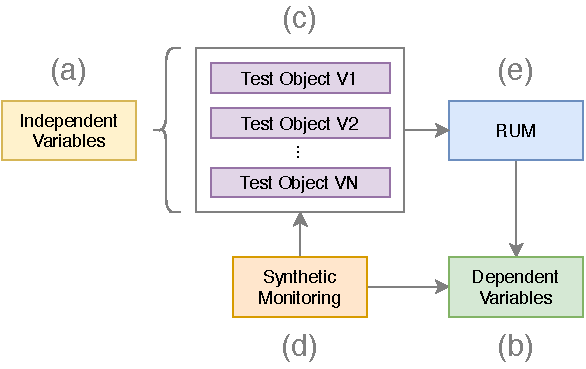
\includegraphics[width=0.8\textwidth]{design.pdf}
\caption{Components from the Controlled Experiment}
\label{figure:design_setup}
\end{center}
\end{figure}

The different parts of the experiment setup will be discussed in more detail below.


% Kohavi 2016: Sample size, collect right metrics, track right users, randomization unit


% --------------------------------------------------

\subsection{(a) Independent Variables}

% [What are they representing]

The IVs reflect two things:
How the tracking script is included into the website, and if another tracking script is present or not.
All IVs and the values they can take are listed in table X:

As described in section X, page tagging is the method of choice when including a tracking script into a website.
Page tagging is in essence the addition of a <script>-Tag to the main HTML document.
Different options exist when adding a script to the main document.
IV 1 describes the the position of the tracking script within the main document.
IV 2 describes the attribute of the included script tag.

If another tracking script, which may interfere with the "main" tracking script, is presented in the main document or not, is reflected in IV 3.

\begin{table}[h]
	\small
	\centering
	\begin{tabular}{ | l | l | l | }
	\hline
	IV \cellcolor{lightgrey} & Describes \cellcolor{lightgrey} & Possible Values \cellcolor{lightgrey} \\
	\hline
	1 & Position of the Tracking Script & top-head, bottom-head, bottom-body \\
	2 & Attribute of the Tracking Script & none, async, defer \\
	3 & Other Tracking Script included & no, yes \\
	\hline
	\end{tabular}
	\medskip
	\caption{Independent Variables}
	\label{table:independent_variables}
\end{table}


The three IVs are discussed in more detail in the following.
Other IVs considered, but not incorporated within the experiment, are discussed in section X.

% -------------------------

\subsubsection{IV 1: Position of the Tracking Script}

% [GA Tracking Code]

This IV may help understand if the position of the tracking script affects the performance.
Google Analytics (GA) is used as the tracking script.
In general, scripts can be included within the head or body section of the HTML document. % https://www.w3schools.com/js/js_whereto.asp
The GA documentation suggests that the GA script "should be added near the top of the <head> tag and before any other script or CSS tags".
% cite https://developers.google.com/analytics/devguides/collection/analyticsjs
Some details about the GA script are given in section X.

% [Other examples]

Other RUM vendors propose a similar position:
Hotjar suggests that "Paste the Tracking Code into the <head> section of your website."
And Akamai says for there tracking tool boomerang:
"Paste the following code snippet into every page of your site at the top of the HEAD, but after sensitive META tags."
% https://developer.akamai.com/tools/boomerang#dealing-with-script-error

The three possible positions of the tracking script, top-head, bottom-head, and bottom-body, are visualized in appendix X.


% https://speedcurve.com/setup/lux/
% SpeedCurve tracking script position: To add real user monitoring (RUM) to your site, paste this snippet at the top of the <HEAD> tag on your pages.

% Grigorik Conference Talk https://www.youtube.com/watch?v=PkOBnYxqj3k&ab_channel=IlyaGrigorik
% And slides https://www.igvita.com/slides/2013/fluent-perfcourse.pdf


% -------------------------

\subsubsection{IV 2: Attribute of the Tracking Script}

The IV 2 is about the attribute of tracking script tag.
As explained in section X, possible attributes, next to have no attribute, are async and defer, and attributes are not applied on inline scripts.

As the GA script is included inline, different attributes should not affect the behaviour of the website nor its performance.
This IV should verify if this statement holds true and it is expected that changing this variable has no impact on performance.

The three attributes none, async, and defer are visualized in appendix X.


% -------------------------

\subsubsection{IV 3: Other Tracking Script is included}

Many websites use more than one tracking script to collect user data or even resort to custom tracking solutions.
Adding and loading another script within the website will increase the page weight, which leads to more requests and bytes, and depending for example on the network speed, loading an additional resource may impact performance badly.

The other script should not be any kind of script, but also a RUM solution, which has the objective to collect and report user data.
This IV is binary and models if another tracking script is included or not.
Changing this variable may capture if multiple tracking scripts interfere with each other.

Hotjar will be used as the additional tracking script.
The two variants, one with an additional script and one without, are visualized in appendix X.

% footnoe hotjar

% -------------------------

\subsubsection{Other IVs not considered but worth mentioning}

Many other IVs could be chosen and they could reflect variables of the tracking script itself, the website, or the infrastructure around it.

% [Script]

As for the additional IVs for the tracking script, other variables could reflect the quality or complexity of the tracking script, e.g., what kind of user data is collected and in what quantity.
Other variables may reflect the file size of the script, or compare different versions and implementations of the same RUM script.

% [Website]

Possible variables for the website may reflect implementation details, how the code is structured, which libraries are used, how many resources such as images and videos are being loaded, how they are arranged, how the CSS is handled, etc.

% [Infrastructure]

And in terms of infrastructure, IVs may model which servers are being used, which webservers run on them, the condition of the network, the device of the end users, or his operating system, browser version, and so on.
Especially on a website and infrastructure level, nearly countless IVs are imaginable.


% -------------------------

\subsubsection{Possible Variations of the Independent Variables}

% [Variants]

When putting the three defined IVs "Position", "Attribute", and "Other Script" together, different possible combinations emerge as displayed in table X.
The variants A1 and OS2 are redundant and will be dismissed as their IV configuration is already represented in variant P1.

\begin{table}[h]
	\small
	\centering
	\begin{tabular}{  | c || c | c | c | } 
	\hline
	Variant & Position & Attribute & Other Scripts \\
	\hline \hline
	Variant P1 & top-head & \cellcolor{lightgrey} none & \cellcolor{lightgrey} no \\
	   Variant P2 & bottom-head & \cellcolor{lightgrey} none & \cellcolor{lightgrey} no \\
	   Variant P3 & bottom-body & \cellcolor{lightgrey} none & \cellcolor{lightgrey} no \\
	  \hline
	   \sout{Variant A1} & \cellcolor{lightgrey} \sout{top-head} & \sout{none} & \cellcolor{lightgrey} \sout{no} \\
	   Variant A2 & \cellcolor{lightgrey} top-head & async & \cellcolor{lightgrey} no \\
	   Variant A3 & \cellcolor{lightgrey} top-head & defer & \cellcolor{lightgrey} no \\
	  \hline
	  \sout{Variant OS1} & \cellcolor{lightgrey} \sout{top-head} & \cellcolor{lightgrey} \sout{none} & \sout{no} \\
	  Variant OS2 & \cellcolor{lightgrey} top-head & \cellcolor{lightgrey} none & yes \\
	  \hline
	\end{tabular}
	\medskip
	\caption{Possible Test Object Variants when combining the IVs.}
	\label{table:test_object_variants}
\end{table}


% [What are the Variants]

The variants themselves are different index.html files from the test website.
The difference between the variants are only the options and position of the tracking script, as described above.
The rest of the test website is remaining the same over all variants.
How the test website is constructed, is discussed below.

% [Evaluation/Comparison]

For evaluation, I will compare the different possible values of one IV with each other, while the values of the other IVs remain unchanged.
For example, the different positions (IV 1) are compared with each other, while the attribute (IV 2) and whether or not another script is included (IV 3) remain the same for all positions.
This is needed in order to measure the impact when changing one IV.
Variants which are not from the same subgroup are not compared with each other, e.g. variant A2 will not be compared to variant OS2.


% --------------------------------------------------

\subsection{(b) Dependent Variables}

The dependent variables measure the outcome of the change in IVs with respect to web performance.
They are web performance metrics.
The synthetic monitoring and RUM solutions implemented in the experiment measure and deliver the dependent variables.

The dependent variables are visualized in order to facilitate the interpretation of the data.
Considered dependent variables (web performance metrics) are common web performance metrics as described in section X, such as page weight, navigation timing metrics such as TTFB and PLT, and user-centric metrics such as Speed Index or LCP.


% -------------------------------------------------------------------------
% -------------------------------------------------------------------------

\subsection{(c) The Test Object: An E-Commerce Website}

% [Difficulty]

In the real world, each website is unique and follows its own design and architecture principles.
The difficulty for conducting research on websites such as within this thesis, is to find a common ground or general website that approximates real world examples as good as possible.

%TODO add best would be real life scenario ?

% Mimic the website is one thing, but also all other aspects should be fairly similar: infrastructure (hosting), hardware used, network speed, traffic, etc.
% This experiment/test is only an approximation and can serve as a starting point for further investigations

% Ideal: Use a real website. Is not possible


% [Goal]

One goal of this thesis is to create a test website which mimics a real life e-commerce website as good as possible.
Multiple ideas to achieve this goal are presented and discussed in the following.


% --------------------------------------------------------

\subsubsection{Minimal Website}

% [Idea]

The idea of the minimal website is to have a clean, laboratory-like environment which is in full control of the tester.
The minimal website is constructed without any content but only a link to an external script, which represents the tracking script.
The script itself has only place holder content which adds bytes to the file size, but does not execute any logic.
    
% [Setup]

The website is hosted, like all following test websites, on GitHub Pages, which is a quick, easy and fast way to deploy a website onto a real server.
The source code for the minimal website is available on GitHub, and the page is deployed to https://aramovski.github.io/.
% footnote : https://github.com/aramovski/aramovski.github.io
% Footnote https://pages.github.com/ [30.08.2021]

% [Evaluation]

The benefit of this approach is that the tester has a lot of control about the website, as there are not many complex coherences or variables within the website itself.
The three discussed IVs can easily be changed.
In addition, the script file size can be changed quickly.
As a downside, the minimal website is too far away from any real world website, e.g. no images or other resources are requested.
Also, it does not cover any e-commerce scenario.
Hence, this idea has been withdrawn.


% --------------------------------------------------------

\subsubsection{Median Website}

% [Idea]

The idea of the median website is to construct a website which represents an "average" website as good as possible.
The median website is created with a median page weight.
This means, it has an average amount of requests and bytes for each resource type such as images, fonts, or videos.
The data for the median values is taken from HTTPArchive.


% [Setup]
% website: mimic page weight as reported on http archive
% source. https://github.com/aram-yesildeniz/median/tree/gh-pages
% Hosting: github pages: https://aram-yesildeniz.github.io/median/

% [Evaluation]
% Only good as a POC: Show that changing independent variables X affect result
% too far away from reality
% maybe compare with real website ?


% 2011 Butkiewicz: Correlation between website complexity and its performance:
% -> Therefore it makes sense for me to use http archive inspired website approach, since page weight / page complexity impacts performance
% - Measures impact of website complexity on performance
% - Finds out that top 5 metrics that determine performance are:
% total number of objects loaded,  the number of these objects that are Javascripts,  the total web- page size,  and the number of servers and origins contacted in loading objects on the page.


% 2011 Grigorik Anatomy of modern web application
% - Chart with changes on time: apps are growing


% 2014 Hogan basics-of-page-speed/ What Is the HTTP Archive?


% --------------------------------------------------------

\subsubsection{WordPress Website}

% [Idea]

The idea of the WordPress website is to leverage one of the most widely used website building frameworks in order to cover many real world examples.
WordPress powers nearly...
% Show usage of WordPress with some statistics: Why is it so verbreitet

% [Plugins]
% Explain Plugin system

% WooCommerce

% [Setup]
% Explain Setup on localhost with wocommerce and GA plugin

% [Evaluation]
% Elaborate why this idea was not used



% --------------------------------------------------------


\subsubsection{Mirroring a complete e-commerce website}


% [Why]

% Close to reality as possible


% Idea: Close to reality as possible
% Problems when mirroring a website
% Elaborate why this idea of mirroring complete website was not used
% I used mock of start page of otto, which works fine
% Compare original otto website with mock


% Why Otto and Zalando ?Which website / shop to clone? Show some statistics about biggest e-commerce websites in germany




% [Setup]

% Tool support to mirror / download complete website: httrack and chrome plugin
% Use free hosting service to serve website

% Otto first try
% Zalando final version

% [Evaluation]
% see evaluation chapter


% --------------

\paragraph{Otto}


% [Manual Adjustments]

% Manual adjustments needed:
% - Move everything to test folder because top domain is /otto


% What did not work (mostly 404s):
% - user-set-consent-id-cookie: Cookie with name consentId is not set, user-set-consent-id-cookie returns therefore 404
% - subscribeToNewsletterSnippetContent: Change path did not work...
% - amount.json: Not found, also wl\_miniWishlistAmount in local storage does not created
% - a\_info: Mock a\_info response json does not work...

% - footer
% - userTiming


% WPT RV is returning empty csv when 404s are encountered.
% Therefore i mock the missing ressources so that WPT can run bulk tests successfully.

% - mock image sprite\_all\_1ba408b2.png

% - create empty file called user-set-consent-id-cookie

% - change path for subscribeToNewsletterSnippetContent: This will remove the cookie banner... but then WPT works



% -------------------

\subparagraph{Comparison to original webpage}

% Maybe use here just WPTs comparison tool

% Show some diagrams here
% The other diagrams with Zalando should go into evaluation chapter



% -----------

\subparagraph{Problem with Caching and Repeat View}

% - Problem with RV, Caching:
% Otto sets request headers to cache-control: no-cache which means that RV basically downloads all resources again.
% The mock is hosted on Github, where the cache-control header is set to ...
% It is not possible to change the github request headers. We can modify the http request headers via html, but this is not a clean solution.
% Therefore I use a different e-commerce website which does not shut down caching so that the RV results are more similar.

% Ideally I would host the mock website on a similar infrastructure as the original site with the same webserver configuration. This is for a masters thesis not feasible.

% Not possible to set cache control in html meta tag https://html.spec.whatwg.org/multipage/semantics.html#attr-meta-http-equiv


% --------------------------------------------------------

\paragraph{Zalando}

% [Why]

% Idea: It looks like zalando page does not has that many cache-control headers, therefore it may be easier to clone so that RVs are more similar.

% [Setup]

% use plugin to download page
% host it on github pages

% [Evaluation]


% add screenshots of original vs test
% see evaluation chapter


\begin{figure}
	\centering
	\begin{subfigure}{.5\textwidth}
		\centering
		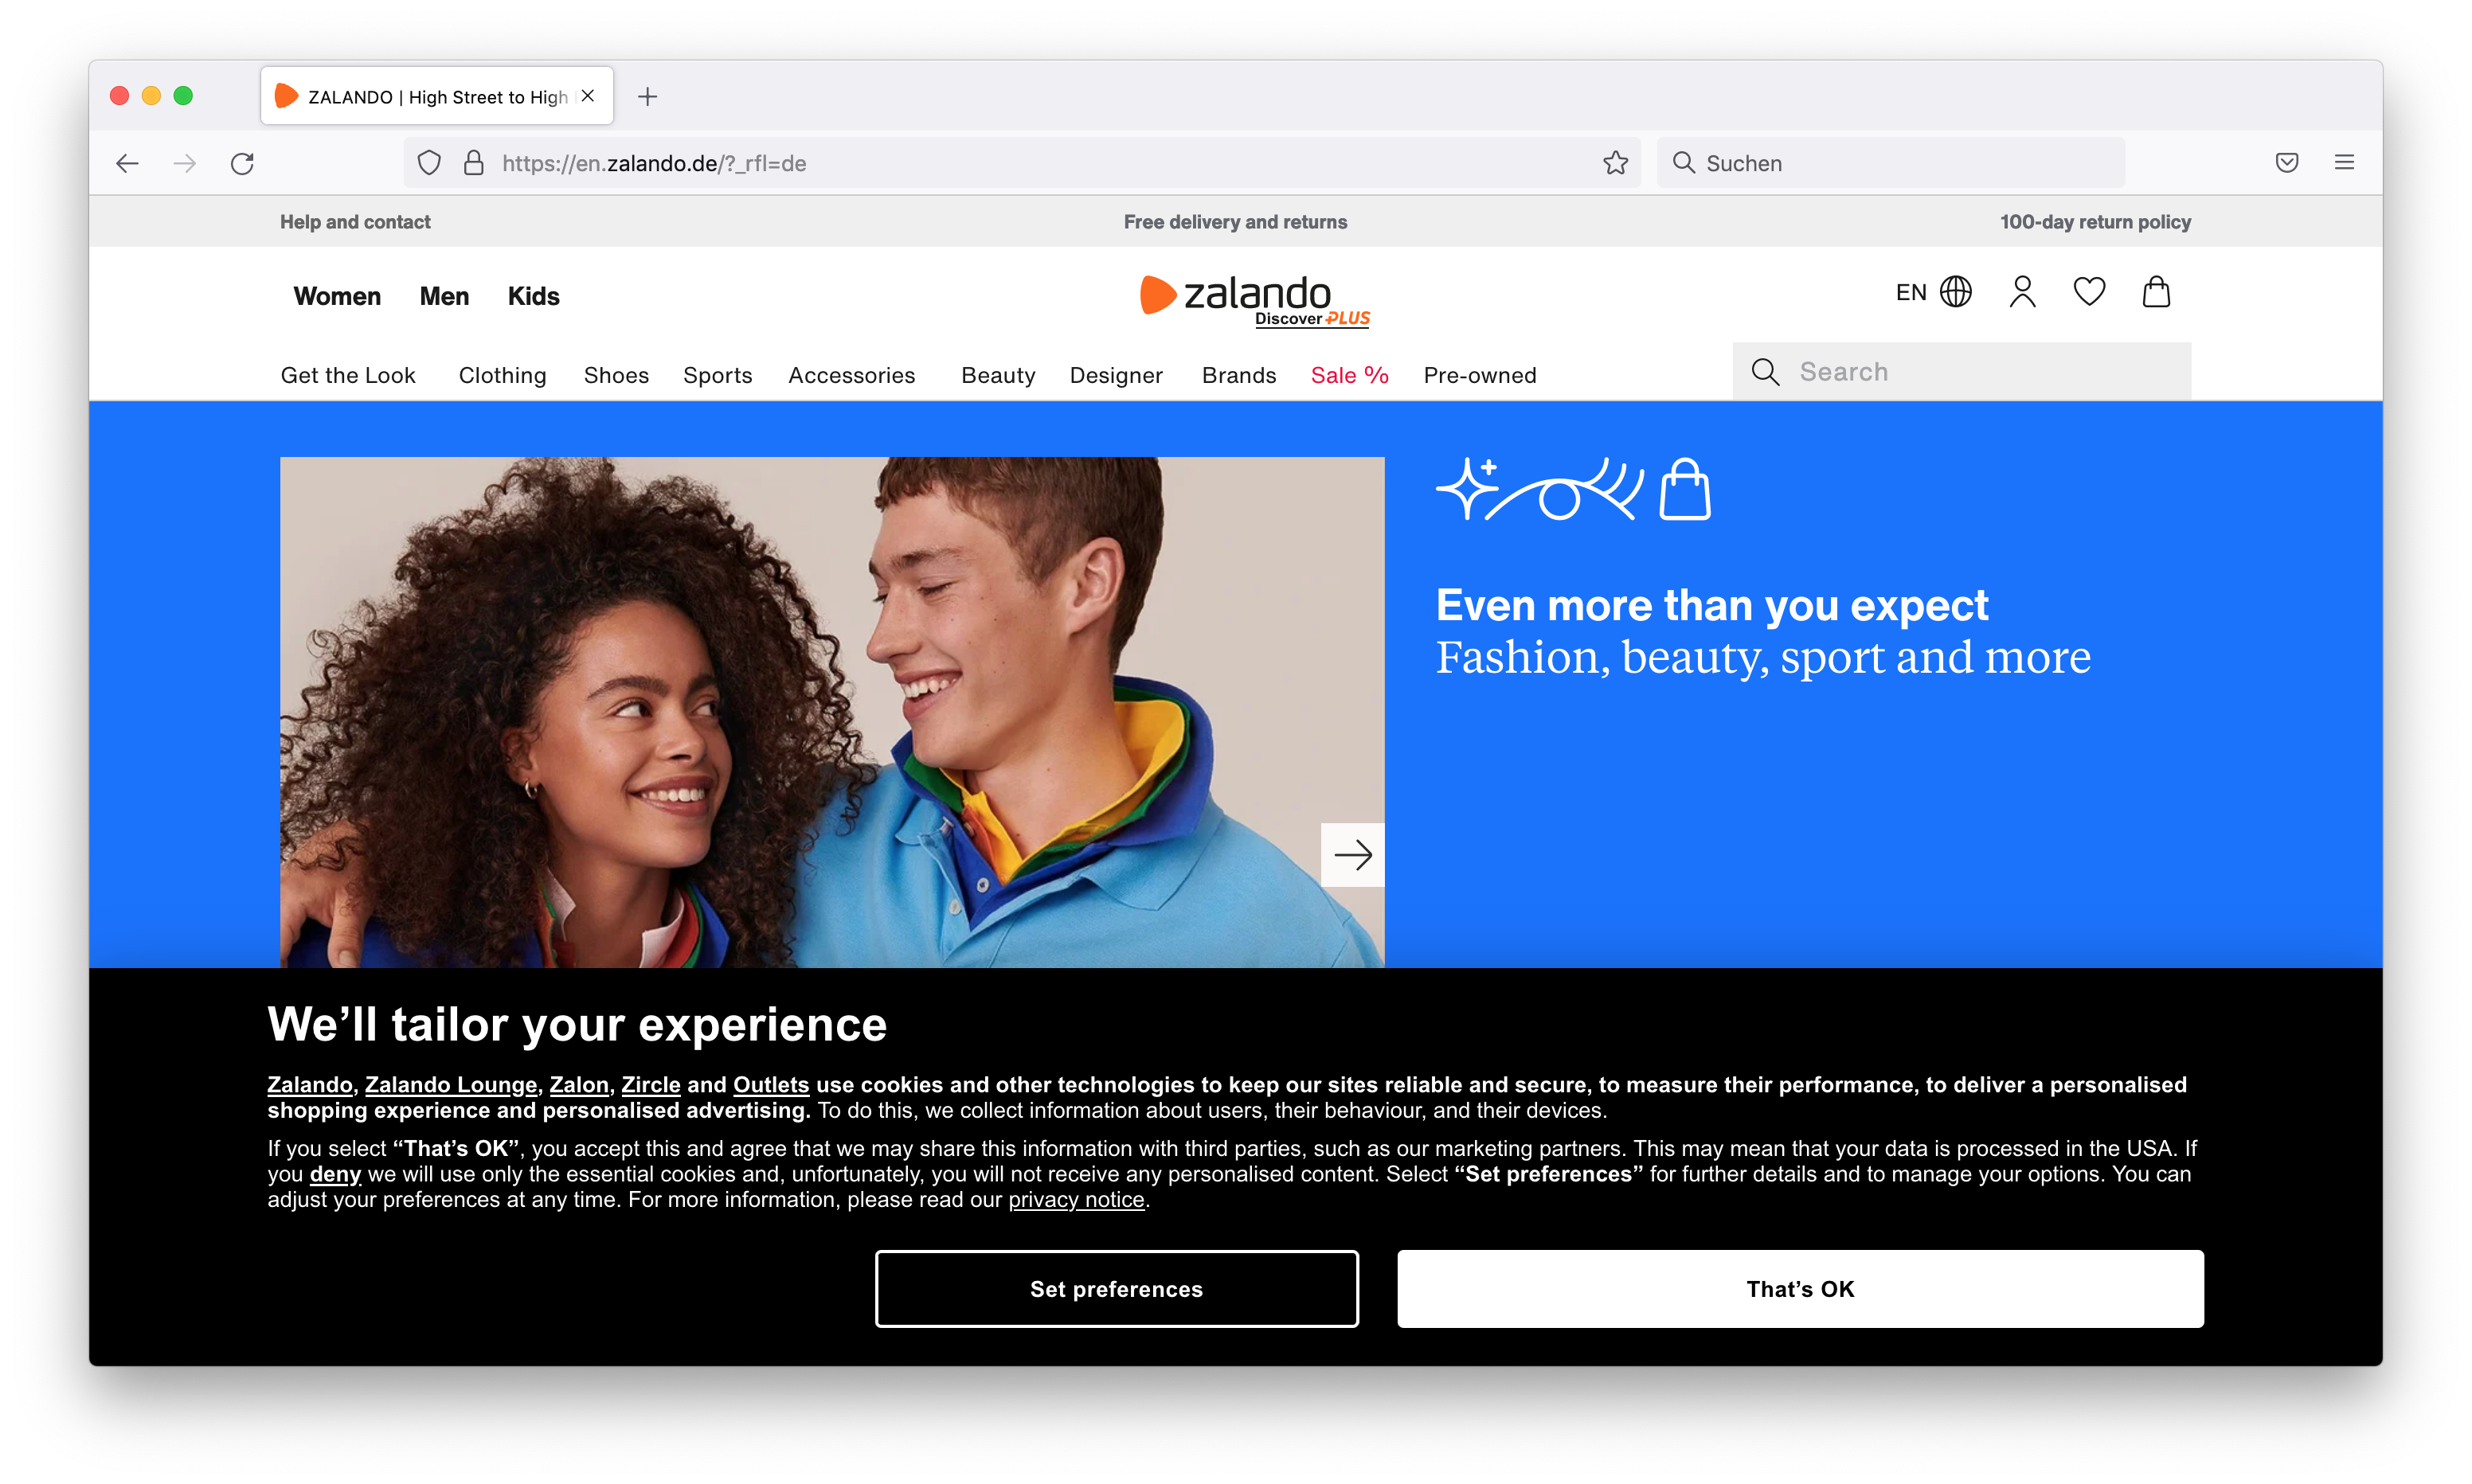
\includegraphics[width=1\linewidth]{original_screenshot.png}
		\caption{https://www.zalando.de/}
		\label{fig:sub1}
	\end{subfigure}%
	\begin{subfigure}{.5\textwidth}
		\centering
		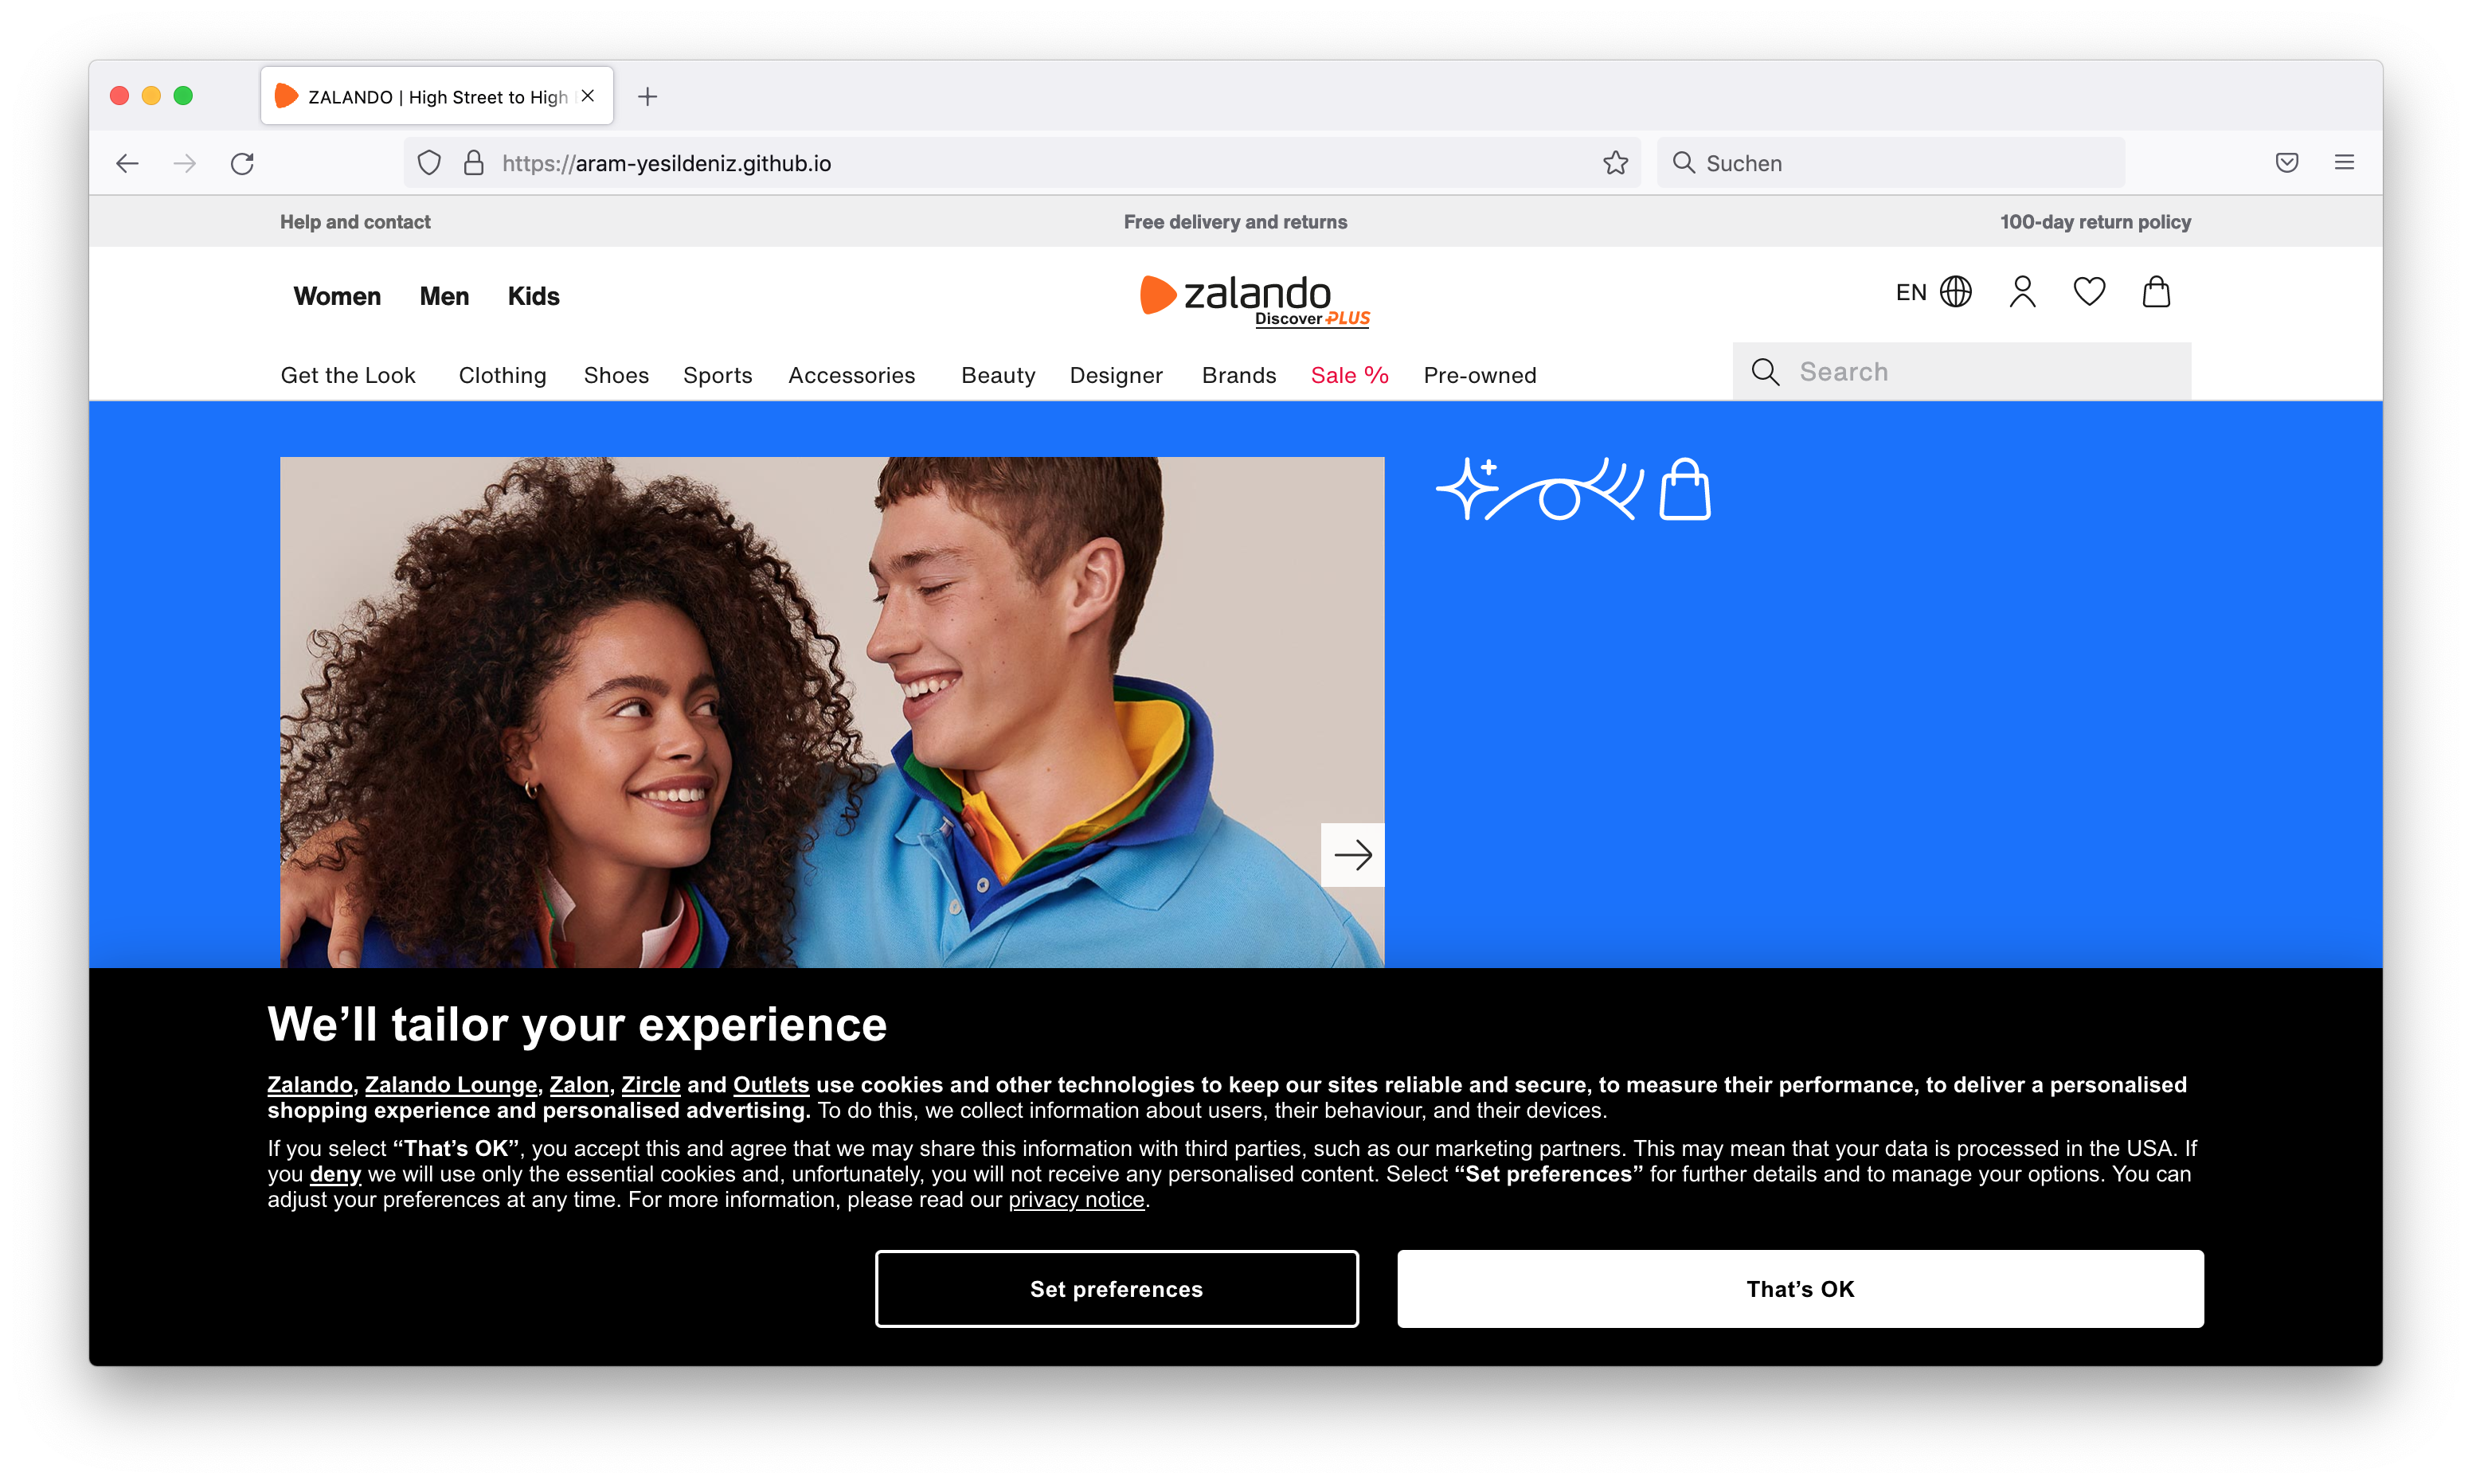
\includegraphics[width=1\linewidth]{test_screenshot.png}
		\caption{https://aram-yesildeniz.github.io/}
		\label{fig:sub2}
	\end{subfigure}
	\caption{Original vs Test Object}
	\label{figure:plt_original_test}
\end{figure}





%TODO add some comparison table? like all ideas, with columns such as "control", "complexity", "generaliseabilty", etc. ?


% --------------------------------------------------


\subsection{(d) Synthetic Monitoring: Create Traffic and Collect Data}

% Synthetic monitoring: Double role: creats traffic which is captured by RUM, and also measured the website

% I want to collect Lab and field data for dependent variables for comparison
% This setup is a special case because lab bots (e.g. WPT) simulate at the same time real users for RUM data


% -------------------------------------

\subsubsection{WebPageTest}

% [Setup]

% Possibilites:
% use public version
% API

% Private:
%- preconfigured Amazon Web Services (AWS) AMIs
%- localhost Docker


\paragraph{Configuration}

% already described in section X.

% [FV vs RV]

% First View: "First View refers to the cold cache setup in which nothing is served locally"
%Repeat View: "Repeat View refers to the warm cache containing everything instantiated by the first view" (2016 Using WPT p. 62)


\begin{table}[h]
	\small
	\centering
	\begin{tabular}{  | c | c | } 
	\hline
	\cellcolor{lightgrey} Configuration Setting & \cellcolor{lightgrey} Option \\
	\hline
%	Test Location & Test Location \\ 
	Browser & Chrome \\
	\hline
	Connection & LAN (connection speed is determined by hotspot) \\
	Desktop Browser Dimensions & default (1366x768) \\
	Number of Tests to Run & 1 \\
	Repeat View & First View and Repeat View \\
	Capture Video & True \\
	Keep Test Private & False \\
	Label & none \\
	\hline	  
	Advanced Tab & Nothing selected \\
	Chromium Tab & Capture Dev Tools Timeline selected  \\
	Auth, Script, Block, SPOF, Custom Tabs & Nothing  \\
	Bulk Testing Tab & URL of the test website $x$ times according to test plan \\
	\hline
	\end{tabular}
	\medskip
	\caption{WPT Configuration}
	\label{table:wpt_configuration}
\end{table}



% ----------------------


\paragraph{Traffic Shaping}

% [Why]

% Network Condition is very important for performance
% Already described in section X issue with Latency vs Bandwidth

% Overview table with different settings:
% https://developer.mozilla.org/en-US/docs/Web/Performance/Understanding_latency


% Important to have stable and realistic network condition
% Chromes tool is not the best for this % see blogpost https://calendar.perfplanet.com/2016/testing-with-realistic-networking-conditions/


% [Network Link Conditioner]

% Private WPT Instance docker on mac does not allow traffic shaping functionality from WPT
% One approach: I use Network Link Conditioner from Apple to slow down the whole machine. See in same blogpost that Patrick highly recommends this
% WPT also slows down their whole machines % https://forums.webpagetest.org/t/measure-internet-speed/11593
% In general internet connection is very unstable. If i run network link conditionier with e.g. DSL each speedtest gives different results. And other test platforms such as fast.com gives also different result.
% i will use the durchschnitt in germany which seems to be 40 mbit per second. or actually i use LTE profile from network conditioner which is 50 mbit per second 


% [Hotspot]

% Solution: Use Mobile Hotspot with 50 mbit/s
% as long as internet connection is stable along all tests, it should not make a big difference because i compare the different variants. Therefore internet connection will fall out of the equation


% ----------------------

\paragraph{Usage of the Bulk Test Feature}


% Bulk testing is a feature for private instances only
% actually gives pretty nice comparison graphics
% Misuse this feature to test the same website X times

% Measured metrics are exposed through a variety of files
% Ill download csv files Summary and detail ? TODO check again how this is called

% keep in mind that FV and RV for one test are directly next to each other
% so to get data for all FVs, i would need data from rows 1 3 5 etc

% i use this for quick comparison of original to test object


% --------------------------------------------------


\subsection{(e) Real-User Monitoring: Google Analytics}

% 2 functions: RUM itself is represented by the script, so it is basically the object where the IVs are applied to
% but also its used to collect data

% Setup: Use Unversial Analytics
% Set sample rate to 100% for speed metrics

% show code here

% Data: could get it from GA dashboard / reports
% but ill use the API to fetch the data more easily: https://aram-yesildeniz.github.io/google-analytics/

% what exactly is the script doing? https://developers.google.com/analytics/devguides/collection/analyticsjs/


What is the GA script doing?
Actually, it creates another async script tag which loads the actual analytics JS.
So basically it should not really play a role where we place it.
Evaluation will show.

What does the code snippet do?
Basically the sync part is only..
It creates another script tag which is async and which loads the tracking code.

This script is an inline script, as it does not have any src attribute.
In theory,  async and defer attributes on inline scripts are ignored, as explained in section X.
"Inline JavaScript script tags ignore the defer or async attribute"
As the "wrapper" snippet is a inline script (no src attribute), the attributes on this script tag should not have any effect.



% what exactly is the script doing? https://developers.google.com/analytics/devguides/collection/analyticsjs/


% where to include: https://developers.google.com/analytics/devguides/collection/analyticsjs/
% The Google Analytics tag should be added near the top of the <head> tag and before any other script or CSS tags



% ------------------------------------------------------------------------------------------
% ------------------------------------------------------------------------------------------


\section{Conducting the Experiment}


% [Schedule Runs]

% The Google Analytics code is more or less fixed and there are no configurations.
% It would be possible to change config of script, e.g. change sample rate, track other metrics etc.
% But it is not possible to change default tracking behaviour (?)

% How the script is included into the file should reflected withing Website Variations

% I will use only one WPT Configuration for all tests.
% Other WPT config can be used in future work, e.g. emulate mobile device.


\begin{table}[h]
	\small
	\centering
	\begin{tabular}{ | l | l | l | l | } 
	 \hline
	  Variant \cellcolor{lightgrey} &  Date \cellcolor{lightgrey} & Traffic Shaping \cellcolor{lightgrey} & Runs \cellcolor{lightgrey} \\
	  \hline
	  Original Website & 2021-05-28 & 50 Mbit/s & 500 \\
	  Mock without GA included & 2021-05-29 & " & " \\
	  \hline
	  Variant P1 & 2021-05-30 & " & " \\
	  Variant P2 & 2021-05-31 & " & " \\
	  Variant P3 & 2021-06-02 & " & " \\
	  \hline
	  Variant A2 & 2021-06-04 & " & " \\
	  Variant A3 & 2021-06-09 & " & " \\
	  \hline
	  Variant OS2 & 2021-06-03 & " & " \\
	  \hline
	  \end{tabular}
	\medskip
	\caption{Test Runs}
	\label{table:test_runs}
\end{table}


% [Procedure]

\begin{itemize}
\item Deploy variant of index.html by pushing to GitHub
% \item Start Network Link Conditioner with specified config on local machine
\item Test internet speed with speedtest-cli
\item Start local WPT server and agent
\item Configure WPT according to specified setup and add list of urls to bulk test interface
\item Run test
\item When finished, download summary csv file
\item On GA helper site, fetch and download data for the current day
\end{itemize}


% [Data Collection]


% [Data Analysis]

% those files are then used to analyse  and visualize data
% python code footnote github


% [Transition]

% Now lets see the data in chapter X Evaluation

\chapter{Evaluation}


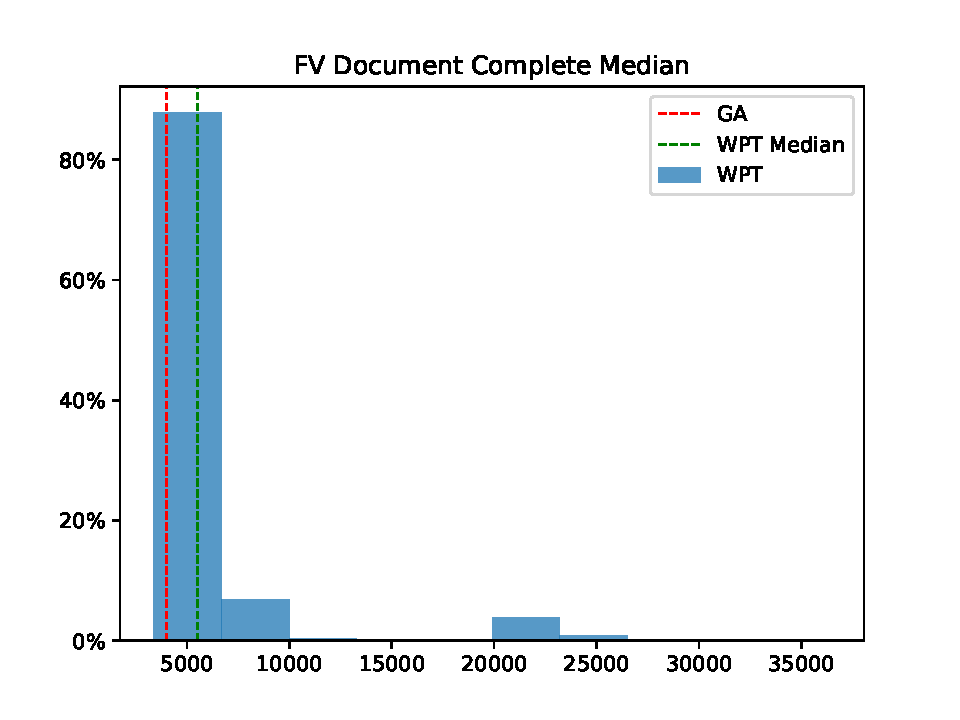
\includegraphics[width=1\textwidth]{test}


\begin{itemize}
	\item Last chapter...
	\item This chapter: Describe shortly all sections from this chapter
	\item In the next chapter...
\end{itemize}




% https://hpbn.co/primer-on-web-performance/#analyzing-real-user-measurement-data



% ----------------------------------------------------------------------------------------------------
% ----------------------------------------------------------------------------------------------------


\section{Test Results}

\subsection{Metrics for Evaluation}

Page Weight: Measured by WPT:
- bytes
- bytes uncompressed
- Requests


Technical Timings / API: Measured by WPT and GA:
- page load time
- domain lookup time
- page download time
- redirection time
- server connection time
- server response time
- Dom interactive time
- Dom content loaded time

Visual Metrics / Web Vitals: Measured by WPT
TODO Measure also with GA / own script ??:
- CLS
- FCP
- FMP
- LCP
- SI

- Visually complete ?
- Time  to Interactive ? Is this the same as DOM interactive time ?

Core Web Vital FID ?? -> Can not be measured without real users...

From WPT bulk section. Also include this somewhere for comparison ?:
- Filmstrips ?
- Waterfall ?
- Visual Progress ?
- Layout Shifts ?



\subsection{Original vs Mock Plain}



\subsection{Mock Plain vs Position 1 (which is default position of GA: Check this again!)}
TODO rename this like with GA true false ?



\subsection{Position 1 vs 2 vs 3}



\subsection{Attribute 1 vs 2 vs 3}



\subsection{Other script True vs False}







% ----------------------------------------------------------------------------------------------------
% ----------------------------------------------------------------------------------------------------


\section{General}

\begin{itemize}
    \item For each attempt, describe: Threats to validity, generalizability
\end{itemize}

generalizability: meine Daten zeige nur für Chrome, MacBook, diese Geschwindigkeit etc.
Und auch nur für diese Test-Website
Die Schwierigkeit der Generalisierbarkeit ist eines der grössten Probleme bei dieser Fragestellung


% TODO get rid of this? Maybe just evaluate all other apporaches quickly in approach section?

\section{Plain / Skeletal Website}

\begin{itemize}
\item Information gained from this experiment
\item Limitations and questions which can not be answered with this approach
\end{itemize}


\section{Mirroring}


\section{HTTP Archive inspired website}

\begin{itemize}
\item Information gained from this experiment
\item Meaning and interpretation of the collected data
\item Limitations and questions which can not be answered with this approach
\end{itemize}





% TODO rework sections below. Here i dont need to present all options / results from WPT again but rather my results ??

\section{WebPageTest Bulk Tests}

\begin{itemize}
\item Bulk testing is a feature for private instances only
\item Misuse this feature to test the same website X times
\end{itemize}


\subsection{Bulk Test Overview: Description of test result page}

\begin{itemize}
\item Each test has Test ID: YYMMDD\textunderscore random\textunderscore random
\item Test results after bulk test available under \url{http://localhost:4000/result/{testID}/}
\item For each test run, following data is available:
	\begin{itemize}
	\item Link to test results: Test result page as same as for single test run
	\item Median load time (First view)
	\item Median load time (Repeat view)
	\item Median Speed Index (First View)
	\item Raw page data (file: [TestID\textunderscore summary.csv]
	\item Raw object data (file: [TestID\textunderscore details.csv])
	\item Http archive (.har) (file: json)
	\end{itemize}
	
\item Average First View Load Time
\item Average Repeat View Load Time
\item Combined Raw: Page Data  (file: [TestID\textunderscore summary.csv])
\item Combined Raw: Object Data (file: [TestID\textunderscore details.csv]). For 100 test runs, this file is appr. 20 MB, 24432 rows, 76 columns. 
\item Aggregate Statistics (file: [TestID\textunderscore aggregate.csv])
\end{itemize}


\subsection{Summary File for one Test}

\begin{itemize}
\item Contains 6 rows: 3 test runs: for each test runs 1x first view and 1x repeat view
\item Rows 1, 3, 5 contain FV, rows 2, 4, 6 contain data for RV
\end{itemize}

\subsection{Aggregate Statistics File}

\begin{itemize}
\item Contains aggregated data from bulk test
\item One row for each test run: For 100 URLs in bulk test will be 100 rows in csv
\item Each metric is available with Median, Average, Standard Deviation, Min, Max
\item Metrics are available once from FV and once for Repeat View
\item Metrics:
	\begin{itemize}
	\item Successful Tests
	\item Document Complete
	\item Fully Loaded
	\item First Byte
	\item Start Render
	\item Bytes In (Doc)
	\item Requests (Doc)
	\item Load Event Start
	\item Speed Index
	\item Last Visual Change
	\item Visually Complete
	\end{itemize}
\item => For metric details, see Terms and Definitions
\end{itemize}


\subsection{Compare Section}

WPT has a feature to compare multiple tests.
Accessible under compare URL: \url{http://localhost:4000/video/compare.php?tests={TestID},{TestID},...}

The compare page contains:

\begin{itemize}
\item Film strip
\item Waterfall diagram
\item Visual Progress diagram
\item Timings diagram:
	\begin{itemize}
	\item Visually Complete (First View Visually Complete Median)
	\item Last Visual Change
	\item Load Time (onload)
	\item ...
	\end{itemize}
\item Cumulative Layout Shift diagram
\item Requests diagram
\item Bytes diagram
\item Visually complete
\item Last Visual Change
\item Load Time (onload)
\item Load Time (Fully Loaded)
\item DOM Content Loaded
\item Speed Index
\item Time to First Byte
\item Time to Title
\item Time to Start Render
\item CPU Busy Time
\item 85\% Visually Complete
\item 90\% Visually Complete
\item 95\% Visually Complete
\item 99\% Visually Complete
\item First Contentful Paint
\item First Meaningful Paint
\item Largest Contenful Paint
\item Cumulative Layout Shift
\item html Requests
\item html Bytes
\item js Requests
\item js Bytes
\item css Requests
\item css Bytes
\item image Requests
\item image Bytes
\item flash Requests
\item flash Bytes
\item font Requests
\item font Bytes
\item video Requests
\item video Bytes
\item other Requests
\item other Bytes
\end{itemize}







\section{Internal, external validity}


\begin{itemize}
\item At this point, i have the data collected and can analyse it
\item The quality and quantity of the data needs to be discussed
\item Quality: There are chances that some data are malformed, e.g. because internet connection was bad, etc.
\item Quantity: Is the amount of data sufficient to make the evaluation generalisable
\end{itemize}


% 2016 Kohavi: Analysis of Experiments


\chapter{Future Work}

\begin{itemize}
	\item Last chapter...
	\item This chapter: Describe shortly all sections from this chapter
	\item In the next chapter...
\end{itemize}


% assess quality of RUM data

\section{Limitations of this thesis}

\begin{itemize}
\item Discussion of unobserved topics
\item Discussion of possible next steps
\end{itemize}

\section{Other measurement tools and metrics}


List of tools and metrics worth investigating
Custom Metrics


\subsection{Google Analytics 4}


\section{Speed Kit}

% 2020 Wolle


\section{PWAs, AMPs, Service Workers, Caching, HTTP2 etc.}

\begin{itemize}
\item Overview of other web technologies and how they could be relevant for further research
\end{itemize}

% Test for Mobile users:
% Mobile shopping on the rise: https://einzelhandel.de/presse/zahlenfaktengrafiken/861-online-handel/4761-bedeutung-der-smartphones-im-onlinehandel
% They are generally more unhappy: https://einzelhandel.de/presse/zahlenfaktengrafiken/861-online-handel/4462-mobile-optimierung-online-shop

% Not covered: Beaconing aspect: When to send data back home, at which time is best, what is tradeoff etc.

% Create a user journey with a script for WPT

\chapter{Conclusion}

\begin{itemize}
	\item Last chapter...
	\item This chapter: Describe shortly all sections from this chapter
\end{itemize}

\begin{itemize}
\item Scope and contribution of this thesis
\item Short summary of each chapter:
	\begin{itemize}
	\item Problem statement and why it is worth to examine research question
	\item Terms and definitions
	\item (Related work)
	\item Approach and evaluation of practical work
	\item Future work
	\end{itemize}
\end{itemize}


- Several topics wurden bearbeitet in this thesis, such like mocking a website for testing purposes, literature review, metrics taxonomy, and the main part which is an experiment 

\chapter{Appendix}

\section{Test Object Variants}


\subsection{IV Position}

\begin{sidewaysfigure}
\begin{multicols}{3}
\begin{center}
\begin{lstlisting}[caption={Position 1}, language=html, numbers=none]
<!DOCTYPE html>
<html>
    <head>
        <!-- Google Analytics -->
        <script></script>
        <!-- End Google Analytics -->

        <title>
        <meta>
        <link>
        <script>
    </head>

    <body>
        ...
    </body>
</html>
\end{lstlisting}
\end{center}

\columnbreak

\begin{center}
\begin{lstlisting}[caption={Position 2}, language=html, numbers=none]
<!DOCTYPE html>
<html>
    <head>
        <title>
        <meta>
        <link>
        <script>
        
        <!-- Google Analytics -->
        <script></script>
        <!-- End Google Analytics -->
    </head>

    <body>
        ...
    </body>
</html>
\end{lstlisting}
\end{center}

\columnbreak

\begin{center}
\begin{lstlisting}[caption={Position 3}, language=html, numbers=none]
<!DOCTYPE html>
<html>
    <head>
        <title>
        <meta>
        <link>
        <script>
        
    </head>

    <body>
        ...
        <!-- Google Analytics -->
        <script></script>
        <!-- End Google Analytics -->
    </body>
</html>
\end{lstlisting}
\end{center}
\end{multicols}
\end{sidewaysfigure}


\subsection{IV 2 Attribute}

\begin{sidewaysfigure}
\begin{multicols}{3}
\begin{center}
\begin{lstlisting}[caption={Attribute 1}, language=html, numbers=none]
<!DOCTYPE html>
<html>
    <head>
        <!-- Google Analytics -->
        <script></script>
        <!-- End Google Analytics -->

        <title>
        <meta>
        <link>
        <script>
    </head>

    <body>
        ...
    </body>
</html>
\end{lstlisting}
\end{center}

\columnbreak

\begin{center}
\begin{lstlisting}[caption={Attribute 2}, language=html, numbers=none]
<!DOCTYPE html>
<html>
    <head>
        <!-- Google Analytics -->
        <script async></script>
        <!-- End Google Analytics -->

        <title>
        <meta>
        <link>
        <script>
    </head>

    <body>
        ...
    </body>
</html>
\end{lstlisting}
\end{center}

\columnbreak

\begin{center}
\begin{lstlisting}[caption={Attribute 3}, language=html, numbers=none]
<!DOCTYPE html>
<html>
    <head>
        <!-- Google Analytics -->
        <script defer></script>
        <!-- End Google Analytics -->

        <title>
        <meta>
        <link>
        <script>
    </head>

    <body>
        ...
    </body>
</html>
\end{lstlisting}
\end{center}
\end{multicols}
\end{sidewaysfigure}








\subsection{IV 3 Other Script}

\begin{sidewaysfigure}
\begin{multicols}{2}
\begin{center}
\begin{lstlisting}[caption={Other Script 1}, language=html, numbers=none]
<!DOCTYPE html>
<html>
    <head>
        <!-- Google Analytics -->
        <script></script>
        <!-- End Google Analytics -->
        




        <title>
        <meta>
        <link>
        <script>
    </head>

    <body>
        ...
    </body>
</html>
\end{lstlisting}
\end{center}

\columnbreak

\begin{center}
\begin{lstlisting}[caption={Other Script 2}, language=html, numbers=none]
<!DOCTYPE html>
<html>
    <head>
        <!-- Google Analytics -->
        <script></script>
        <!-- End Google Analytics -->
        
        <!-- Other Script-->
        <script></script>
        <!-- End Other Script -->

        <title>
        <meta>
        <link>
        <script>
    </head>

    <body>
        ...
    </body>
</html>
\end{lstlisting}
\end{center}
\end{multicols}
\end{sidewaysfigure}


% ------------------------------------------------------------------------------------------------



\subsection{Single Test Raw page data}

WPT Metrics from summary file
\begin{center}
	\small
	\begin{longtable}{ p{0.4\linewidth} | p{0.6\linewidth} }
	Name & Description \\ 
	\hline
        minify\textunderscore total & Total bytes of minifiable text static assets. \\
        responses\textunderscore 200 & The number of responses with HTTP status code of 200, OK. \\
        testStartOffset & ... \\
        bytesOut & The total bytes sent from the browser to other servers. \\
        gzip\textunderscore savings & Total bytes of compressed responses. \\
        requestsFull & ... \\
        start\textunderscore epoch & ... \\
        connections & The number of connections used. \\
        base\textunderscore page\textunderscore cdn & The CDN provider for the base page. \\
        bytesOutDoc & Same as bytesOut but only includes bytes until the Document Complete
event. Usually when all the page content has loaded (window.onload). \\
        result & Test result code. \\
        final\textunderscore base\textunderscore page\textunderscore request\textunderscore id & ... \\
        basePageSSLTime & ... \\
        docTime & Same as loadTime. \\
        domContentLoadedEventEnd & Time in ms since navigation started until document DOMContentLoaded event finished. \\
        image\textunderscore savings & Total bytes of compressed images. \\
        requestsDoc & The number of requests until Document Complete event. \\
        firstMeaningfulPaint & ... \\
        score\textunderscore cookies & WebPageTest performance review score for not using cookies on static assets. \\
        firstPaint & RUM First Paint Time, the time in ms when browser first painted something on screen. It's calculated on the client for browsers that implement this method. \\
        score\textunderscore cdn & WebPageTest performance review score for using CDN for all static assets. \\
        optimization\textunderscore checked & Whether or not optmizations were checked. \\
        score\textunderscore minify & WebPageTest performance review score for minifying text static assets. \\
        gzip\textunderscore total & Total bytes of compressible responses. \\
        responses\textunderscore 404 & The number of responses with HTTP status code of 404, not found. \\
        loadTime & The total time taken to load the page (window.onload) in ms. \\
        URL & The tested page URL. \\
        score\textunderscore combine & WebPageTest performance review score for bundling JavaScript
and/or CSS assets. \\
        firstContentfulPaint & ... \\
        image\textunderscore total & Total bytes of images. \\
        score\textunderscore etags & WebPageTest performance review score for disabling *ETag*s. \\
        loadEventStart & Time in ms since navigation started until window.onload event was triggered (from W3C Navigation Timing). \\
        minify\textunderscore savings & Total bytes of minified text static assets. \\
        score\textunderscore progressive\textunderscore jpeg & WebPageTest performance review score for using progressive JPEG. \\
        domInteractive & ... \\
        score\textunderscore gzip & WebPageTest performance review score for using gzip compression for
transferring compressable responses. \\
        score\textunderscore compress & WebPageTest performance review score for compressing images. \\
        domContentLoadedEventStart & Time in ms since navigation started until document DOMContentLoaded event was triggered (from W3C Navigation Timing). \\
        final\textunderscore url & ... \\
        bytesInDoc & Same as bytestIn but only includes bytes until Document Complete event. \\
        firstImagePaint & ... \\
        score\textunderscore keep-alive & WebPageTest performance review score for using persistent connections. \\
        loadEventEnd & Time in ms since navigation started until window.onload event finished. \\
        cached &  0 for first view or 1 for repeat view. \\
        score\textunderscore cache & WebPageTest performance review score for leveraging browser caching of static assets. \\
        responses\textunderscore other & The number of responses with HTTPS status code different from 200 or 404. \\
        main\textunderscore frame & ... \\
        fullyLoaded & The time (in ms) the page took to be fully loaded — e.g., 2 seconds of no network activity after Document Complete. This will usually include any activity that is triggered by javascript after the main page loads. \\
        requests & List of details of all requests on tested page. \\
        final\textunderscore base\textunderscore page\textunderscore request & ... \\
        TTFB & Time to first byte, which is the duration in ms from when the user first made the HTTP request to the very first byte of the page being received by the browser. \\
        bytesIn & The amount of data that browser had to download in order to load the page. It
is also commonly referred to as the page size. \\
        osPlatform & ... \\
        test\textunderscore run\textunderscore time\textunderscore ms & ... \\
        tester & The ID of tester that performed the page test. \\
        browser\textunderscore version & The browser version. \\
        document\textunderscore origin & ... \\
        document\textunderscore URL & ... \\
        date & Time and date (number of seconds since Epoch) when test was complete. \\
        PerformancePaintTiming.first-paint & ... \\
        osVersion & ... \\
        domElements & The total number of DOM elements. \\
        browserVersion & The browser version. \\
        fullyLoadedCPUms & CPU busy time in ms until page was fully loaded. \\
        browser\textunderscore name & The browser name. \\
        PerformancePaintTiming.first-contentful-paint & ... \\
        base\textunderscore page\textunderscore cname & ... \\
        eventName & ... \\
        os\textunderscore version & ... \\
        base\textunderscore page\textunderscore dns\textunderscore server & ... \\
        fullyLoadedCPUpct & Average CPU utilization up until page is fully loaded. \\
        domComplete & ... \\
        base\textunderscore page\textunderscore ip\textunderscore ptr & ... \\
        document\textunderscore hostname & ... \\
        lastVisualChange & Time in ms until the last visual changed occured. \\
        visualComplete & Time in ms when page was visually completed. \\
        render & The first point in time (in ms) that something was displayed to the screen. Before that user was staring at a blank page. This does not necessarily mean the user saw the page content — it could just be something as simple as a background color — but it is the first indication of something happening for the user. \\
        SpeedIndex & The SpeedIndex score. \\
        visualComplete85 & Time in ms when page was visually completed 85\%. \\
        visualComplete90 & Time in ms when page was visually completed 90\%. \\
        visualComplete95 & Time in ms when page was visually completed 95\%. \\
        visualComplete99 & Time in ms when page was visually completed 99\%. \\
        LargestContentfulPaintType & ... \\
        LargestContentfulPaintNodeType & ... \\
        chromeUserTiming.navigationStart & ... \\
        chromeUserTiming.fetchStart & ... \\
        chromeUserTiming.responseEnd & ... \\
        chromeUserTiming.domLoading & ... \\
        chromeUserTiming.markAsMainFrame & ... \\
        chromeUserTiming.domInteractive & ... \\
        chromeUserTiming.domContentLoadedEventStart & ... \\
        chromeUserTiming.domContentLoadedEventEnd & ... \\
        chromeUserTiming.firstPaint & ... \\
        chromeUserTiming.firstContentfulPaint & ... \\
        chromeUserTiming.firstImagePaint & ... \\
        chromeUserTiming.firstMeaningfulPaint & ... \\
        chromeUserTiming.firstMeaningfulPaintCandidate & ... \\
        chromeUserTiming.domComplete & ... \\
        chromeUserTiming.loadEventStart & ... \\
        chromeUserTiming.loadEventEnd & ... \\
        chromeUserTiming.LargestContentfulPaint & ... \\
        chromeUserTiming.LargestTextPaint & ... \\
        chromeUserTiming.CumulativeLayoutShift & ... \\
        run & The run number. \\
        step & ... \\
        effectiveBps & Bytes per seconds, i.e.: total of bytes in / total time to load the page. \\
        effectiveBpsDoc & Same as effectiveBps but until Document Complete event. \\
        domTime & The total time in ms until a given DOM element (specified via domelement parameter when running a test) was found on the page. \\
        aft & Above the Fold Time (no longer supported). The time taken to load everything in
the viewport above the fold. \\
        titleTime & Total time in ms until page title was set on browser. \\
        domLoading & ... \\
        server\textunderscore rtt & ... \\
        smallImageCount & ... \\
        bigImageCount & ... \\
        maybeCaptcha & ... \\
        bytes.html & ... \\
        requests.html & ... \\
        bytesUncompressed.html & ... \\
        bytes.js & ... \\
        requests.js & ... \\
        bytesUncompressed.js & ... \\
        bytes.css & ... \\
        requests.css & ... \\
        bytesUncompressed.css & ... \\
        bytes.image & ... \\
        requests.image & ... \\
        bytesUncompressed.image & ... \\
        bytes.flash & ... \\
        requests.flash & ... \\
        bytesUncompressed.flash & ... \\
        bytes.font & ... \\
        requests.font & ... \\
        bytesUncompressed.font & ... \\
        bytes.video & ... \\
        requests.video & ... \\
        bytesUncompressed.video & ... \\
        bytes.other & ... \\
        requests.other & ... \\
        bytesUncompressed.other & ... \\
        id & ... \\
        chromeUserTiming.InteractiveTime & ... \\
     \caption{Your caption here} % needs to go inside longtable environment
	\label{tab:myfirstlongtable}
	\end{longtable}
\end{center}



\cleardoublepage



% VERZEICHNISSE (Abbildungen, Tabellen)
% Literatur
\nocite{wiki:wissarbeit}
\bibliographystyle{alphadin}
\bibliography{thesis}
\cleardoublepage




% ERKLÄRUNG
\chapter*{Eidesstattliche Versicherung}
\thispagestyle{empty}
\addcontentsline{toc}{chapter}{Eidesstattliche Versicherung}

Hiermit versichere ich an Eides statt, dass ich die vorliegende Arbeit selbstständig und ohne fremde Hilfe angefertigt und mich anderer als der im beigefügten Verzeichnis angegebenen Hilfsmittel nicht bedient habe.
Alle Stellen, die wörtlich oder sinngemäß aus Veröffentlichungen entnommen wurden, sind als solche kenntlich gemacht. 
Ich versichere weiterhin, dass ich die Arbeit vorher nicht in einem anderen Prüfungsverfahren eingereicht habe und die eingereichte schriftliche Fassung der auf dem elektronischen Speichermedium entspricht.

\noindent Ich bin mit einer Einstellung in den Bestand der Bibliothek des Fachbereiches einverstanden.

\vspace{2cm} 

\noindent Hamburg, den \uline{~~~~~~~~~~~~~~~~~~~~}~~~~~Unterschrift: \uline{~~~~~~~~~~~~~~~~~~~~~~~~~~~~~~~~~~~~~~~~~~~~~~~~~~} 




    
\end{document}